% ==============================================================================
%  $RCSfile: spec.tex,v $, $Revision: 1.58 $
%  $Date: 2003-11-27 17:42:00 $
%  $Author: koppor $
%
%  Description: Master Datei der Spezifikation
%
%  Last-Ispelled-Revision: 1.30
%
% ==============================================================================

\documentclass[a4paper,titlepage,11pt,german,twoside]{scrbook}


\makeatletter

%koma uses \chapter*, but we want to use \chapter
%  changed srcbook.cls-commands
\renewcommand\idx@heading{%
  \twocolumn
  \chapter{\indexname}\@mkboth{\indexname}{\indexname}
}

%Nummerierung soll net so eng aneinanderhaengen
\renewcommand*\l@section{\@dottedtocline{1}{1.5em}{3em}}

\makeatother


\usepackage{../styles/common}

\usepackage{spec}

\usepackage{makeidx}
\makeindex

% subsubsections nummerieren
\setcounter{secnumdepth}{3}

\newcommand\version{Version 1.1\xspace}
%\newcommand\version{\today\xspace}

%\graphicspath{{gui-pictures/}} %OK: it MAY work with graphics. With graphicx, it surely doesn't

% header
\fancyhead{}
\fancyhead[LE,RO]{\slshape \company}
\fancyhead[LO,RE]{\slshape \leftmark}
\fancyfoot[LE,RO]{\thepage{}}
\fancyfoot[LO,RE]{\version}

\begin{document}

% title page
\thispagestyle{empty}
\hfill
\parbox{5.5cm}
{Universit�t Stuttgart\\
Studienprojekt A -- IML Browser\\
\company}

\vspace{3cm}

\begin{center}
  \Huge
  \textsf{Spezifikation}\\
  \vspace{.5cm}
  {\Large\version}\\
  \vspace{3cm}
  
\includegraphics[scale=.74]{../logo}
\end{center}
\newpage

\section*{Versionsgeschichte}

\begin{itemize}

\item Version 1.0 (08.04.2003)

  Diese Version wurde dem Kunden zur Pr�fung 
  im Kundenreview (14.04.2003 - 16.04.2003) vorgelegt.


\item Version 1.1 (22.04.2003)

  Die Korrekturen gem�� dem Kundenreview vom 14.04.2003 bis
  zum 16.04.2003 wurden eingearbeitet.\\
  Die Spezifikation der GSL (in Version 1.0 noch GQSL) wurde in 
  ein separates Dokument ausgelagert (siehe Kapitel 
  \ref {GIANT Scripting Language}).\\
  Diese Version der Spezifikation ging am 22.04.2003 
  zur Abnahme an den Kunden.

\end{itemize}

%%% Local Variables: 
%%% TeX-master: "spec"
%%% End: 


%===============================================================================
%
% ToDo - Aus fertigem Dokument entferenen
%
% \chapter*{ToDo -- nicht in fertiger Spez.}

% Hier Sachen beschreiben, die irgendwie beim Erstellen der Spez.\ 
% beachtet werden sollen.

% % ==============================================================================
%  $RCSfile: todo_spec.tex,v $ 
%  $Date: 2003-04-08 13:28:24 $
%  $Author: squig $ 
%
%  Description: ToDo File f�r die Spezifikation
%
% ==============================================================================

%=======================================================================
\section*{Konfigurationsdatei}
Konfigurationsdatei in extra Kapitel komplett beschreiben
--- was kann konfiguriert werden ?


%===============================================================================
%
% Anforderungen des Kunden
%
\section*{Anforderungen des Kunden}
Anbei die Anforderungen des Kunden gem�� der Email vom 30.01.2003

\begin{itemize}

\item Form: DIN A4, gen�gend Platz f�r Korrektur und handschriftliche 
Anmerkungen


\item Gedruckte Dokumentation + PDF

\item Versionierung: Jedes Dokument erh�lt eine Revisionsnummer, 
Erstellungsdatum wird vermerkt

\item Inhaltliche Form: Jedes Dokument verf�gt �ber ein Inhaltsverzeichnis,
Index ist erw�nscht, Seitenzahlen


\item Referenzen: Konsistente globale Nummerierung f�r alle Dokumente
(lebenslang und f�r immer und ewig)

\item Querverweise (innerhalb des selben Dokuments), 
Referenzen auf weitere Dokumente �ber Seite + Abschnitt

\item Inhalt: Begriffslexikon, Konzepte der GUI, 
Erkl�rungen der GUI zum Beispiel anhand abstrakter Bilder,
Usecases mit Zielsetzung spezifizieren

\item vollst�ndige Abdeckung der Anforderungen an das Produkt

\item pr�zise, knapp

\item Traceability: \\
Spezifikation ist der erste Schritt auf dem langen
(und beschwerlichen) Weg zum fertigen Software-Produkt und
dient als Grundlage f�r das weitere Vorgehen.\\
Entwurf, Implementierung und Test referenzieren sie.
Testf�lle f�r den Systemtest sollen aus der Spezifikation
ableitbar sein.


\item Sprache:\\
Wenn Deutsch als Sprache gew�hlt wird, sollten englische Fach-Begriffe
verwendet werden. (Die selben Begriffe werden in Spezifikation
und Implementierung verwendet.)\\
Keine Eindeutschung.\\
Einheitliche Rechtschreibung.

\end{itemize}


%=============================================================================
%
% Mit Kunden zu kl�ren
%
\section*{Mit Kunden zu kl�rende Punkte}
Alles was noch offen ist.

\begin{itemize}

\item Interaktionssprache von GIANT (insbeondere der GUI und gegebenfalls innerhalb der Konfigurationsdateien) mit Kunden kl�ren (Deutsch oder Englisch).


\end{itemize}

%===============================================================================
%
% Inhaltsverzeichnis
%
\setcounter{tocdepth}{1}
\tableofcontents

%===============================================================================
%
% Einleitung
%
\chapter{Einleitung}
% ==============================================================================
%  $RCSfile: intro.tex,v $, $Revision: 1.14 $
%  $Date: 2003-04-18 19:43:26 $
%  $Author: schwiemn $
%
%  Description:
%
%  Last-Ispelled-Revision: 1.9
%
% ==============================================================================


\section{�ber dieses Dokument}

Diese Spezifikation beschreibt die funktionalen und die nicht-funktionalen 
Anforderungen an den IML-Browser GIANT sowie die Rahmenbedingungen, unter 
denen GIANT lauff�hig sein muss.\\
Dieses Dokument ist Grundlage f�r die weitere Entwicklung von GIANT
innerhalb dieses Projekts, das hei�t im Besonderen f�r das Benutzerhandbuch, 
den Entwurf, die Implementierung und den Test des Softwaresystems. 
Das Dokument ist an die Mitglieder der Projektgruppe sowie an den Kunden und
dessen technische Berater gerichtet.\\
Dieses Dokument ist Vertragsbestandteil f�r die weitere Entwicklung von GIANT 
und somit auch Grundlage f�r die Abnahme des fertigen Produktes.


\section{�ber GIANT -- Graphical IML Analysis Navigation Tool}
\index{GIANT}
\index{IML-Browser}

GIANT ist ein Werkzeug, welches an der Universit�t Stuttgart von der 
CodeFabrik@Stuttgart im Rahmen des Studienprojektes A IML-Browser 
des Studiengangs Softwaretechnik entwickelt wird.\\
Ziel dieser Entwicklung ist es, die bereits bestehende HTML-basierte L�sung 
der Bauhaus Reengineering GmbH \index{Bauhaus-Reengineering GmbH}
f�r IML-Graphen durch ein komfortables graphisches Werkzeug zu erg�nzen. 
GIANT soll es dem Kunden erm�glichen, Teile von gro�en IML-Graphen zu
visualisieren. 
Durch die Unterscheidung der verschiedenen Kanten- und Knotenklassen sollen
dar�ber hinaus auch im IML-Graphen enthaltene Analyseergebnisse �bersichtlich
dargestellt werden k�nnen.\\
Das Produkt soll sich durch einen hohen Grad an Wartbarkeit auszeichnen. 
Dies soll insbesondere dadurch erreicht werden, dass die Anbindung an die 
Bauhaus-IML-Graph-Bibliothek derart vorgenommen wird, dass �nderungen in der
Spezifikation des IML-Graphen, wie z.B. das Einbringen neuer Attribute,
m�glichst keine Wartungsarbeiten an GIANT selbst zur Folge haben.


%===============================================================================
%
% Produkt�bersicht
%
\chapter{Produkt�bersicht}

In diesem Kapitel werden einige grundlegende Konzepte von GIANT 
vorgestellt und kurz beschrieben. Dieses Kapitel
stellt lediglich eine kurze �bersicht dar, die hier 
vorgestellten Konzepte werden weiter hinten 
in diesem Dokument im Detail spezifiziert -- siehe hierzu
auch die Verweise innerhalb dieses Kapitels. 

% ==============================================================================
%  $RCSfile: product.tex,v $, $Revision: 1.5 $
%  $Date: 2003-09-09 22:12:40 $
%  $Author: birdy $
%
%  Description: Beschreibung des Produktes. �bersicht �ber die Funktionen
%               und allgemeine Bedienkonzepte.
%
%  Last-Ispelled-Revision:
%
% ==============================================================================


% ==============================================================================
\section{GIANT Projekte} \index{Projekte} \index{Persistenz}

Innerhalb eines Projektes fasst GIANT Informationen wie
Anzeigefenster und IML-Teilgraphen f�r einen vorgegebenen IML-Graphen
zusammen und speichert diese persistent. Die Zusammenfassung zu
Projekten soll der �bersicht dienen und den Austausch von
Teilergebnissen,
wie z.B. einzelner Anzeigefenster, erleichtern.\\
F�r weitere Informationen zu Projekten siehe Kapitel \ref{GIANT
  Projektverwaltung}.


% ==============================================================================
\section{IML-Teilgraphen und Selektionen}
Hinsichtlich der logischen Zusammenfassung von IML-Knoten und IML-Kanten unterscheidet
GIANT IML-Teilgraphen und Selektionen.

  \subsection{IML-Teilgraphen} \index{IML-Teilgraphen}
  \index{Graph-Knoten} \index{Graph-Kanten} \index{hervorheben} 
  
  Ein IML-Teilgraph ist eine Knoten- und Kantenmenge aus dem
  IML-Graphen mit der Bedingung, dass die Start- und Zielknoten jeder
  Kante Teil der Menge sind. Diese sogenannten Graph-Knoten und
  Graph-Kanten k�nnen in Anzeigefenstern hervorgehoben werden.
  Des weiteren k�nnen die Graph-Knoten und Graph-Kanten von
  IML-Teilgraphen als Fenster-Knoten und Fenster-Kanten in
  Anzeigefenster eingef�gt und layoutet werden. Die IML-Teilgraphen
  sind global in der Anwendung verf�gbar, aber v�llig unabh�ngig von
  den Anzeigefenstern und enthalten insbesondere keine
  Layoutinformationen.

  \subsection{Selektionen} \index{Selektionen}
  Selektionen stellen eine Menge von Fenster-Knoten und Fenster-Kanten
  dar. Selektionen sind immer einem festen Anzeigefenster zugeordnet
  und umfassen nur Fenster-Knoten und Fenster-Kanten des
  Anzeigeinhaltes dieses Anzeigefensters.
  Die Fenster-Knoten und Fenster-Kanten einer Selektion m�ssen keinen
  Teilgraphen bilden, sie d�rfen also auch Fenster-Kanten ohne die
  zugeh�rigen Start- und Zielknoten umfassen.

% ==============================================================================
\section{Anzeigefenster} \index{Anzeigefenster}
Anzeigefenster sind die Fenster von GIANT, in denen eine benutzerdefinierte
Auswahl von Fenster-Knoten und Fenster-Kanten visualisiert wird. 
Es kann beliebig viele
Anzeigefenster geben und jedes Anzeigefenster kann beliebig viele Selektionen
haben.

  \subsection{Pins}\label{Pins} \index{Anzeigefenster!Pins} \index{Pins}
  Da bei gro�en Graphen selten alle zu einem Anzeigeinhalt 
  geh�renden Fenster-Knoten und Fenster-Kanten gemeinsam auf dem Bildschirm
  sichtbar dargestellt werden k�nnen, kann sich der
  Benutzer zu jedem Anzeigefenster eine Liste von Pins anlegen. In den Pins wird
  jeweils die Position des sichtbaren Anzeigeinhaltes und die Zoomstufe
  \index{Zoomstufe}
  gespeichert, so dass zu beliebigen Zeitpunkten die Position des sichtbaren
  Anzeigeinhalts rekonstruiert werden kann.

  \subsection{Visualisierungsstile} \index{Visualisierungsstile}
  Mittels sogenannter Visualisierungsstile kann der Benutzer die
  Darstellung von Fenster-Kanten und Fenster-Knoten auch w�hrend der
  Laufzeit von GIANT beeinflussen.  Da �ber entsprechende XML-Dateien
  verschiedene Visualisierungsstile definiert werden k�nnen, kann
  GIANT so
  an spezifische Problemstellungen angepasst werden.
  Weitere Informationen hierzu sind in Abschnitt \ref{Config
    Visualisierungsstile} zu finden.

\section{Knoten-Annotationen} 
\index{Knoten-Annotationen}

Jeder Knoten kann mit einer textuellen Annotation versehen werden.
Diese Annotation kann in einem Fenster au�erhalb des Anzeigefensters
zur Anzeige gebracht und bearbeitet werden.
F�r weitere Informationen zu diesem Thema siehe Abschnitt \ref{Project Persistenz von
Knoten-Annotationen}.

% ==============================================================================
\section{Anfragen} \index{GSL} \index{Anfragesprache}
Eine vielseitige Anfragesprache -- die GIANT Scripting Language GSL --
stellt nahezu die gesamte Funktionalit�t von GIANT zur Verf�gung und kann 
insbesondere auch zum Aufruf via Kommandozeile
genutzt werden.\\
Die GSL ist unter Kapitel \ref {GIANT Scripting Language} im
Detail spezifiziert.



%===============================================================================
%
% Allgemeines zu den Funktionalen Anforderungen
%
\chapter{Allgemeine Funktionale Anforderungen}

Dieses Kapitel beschreibt die funktionalen Anforderungen an GIANT, die
das System als Ganzes und nicht nur einzelne UseCases betreffen. Dies
sind z.B. allgemeine Bedienkonzepte zur Selektion von Fenster-Knoten und
Fenster-Kanten, sowie das grundlegende Verhalten von GIANT im Fehlerfall.

% ==============================================================================
%  $RCSfile: afa.tex,v $, $Revision: 1.23 $
%  $Date: 2003-04-21 01:13:30 $
%  $Author: schwiemn $
%
%  Description: Beschreibung allgemeiner funktionaler Anforderungen - UseCase
%               �bergreifend.
%
%  Last-Ispelled-Revision: 1.10
%
% ==============================================================================


\section{Fehlerverhalten} \index{Fehlerverhalten}
\label{afa Fehlerverhalten}

Beim Auftreten von Fehlern w�hrend des Betriebs von GIANT werden
die folgenden Konventionen eingehalten. GIANT verh�lt sich bez�glich der 
Fehlerbehandlung konsistent. Das im Folgenden beschriebene Fehlerverhalten gilt 
daher f�r das gesamte System. Abweichungen von diesem Verhalten werden gegebenenfalls 
an der entsprechenden Stelle explizit spezifiziert.

\begin {enumerate}
  \item
  Fehlermeldungen \index{Fehlermeldungen} werden grunds�tzlich �ber
  einen allgemeinen Fehlerdialog ausgegeben 
  (siehe auch \ref {GUI Ausgabe von Fehlermeldungen}). 
  Ist dies nicht m�glich, wird die Fehlermeldung
  �ber die Kommandozeile ausgegeben.

  \item
  Sollten mehrere Fehler, wie z.B. Eingabefehler, gleichzeitig auftreten,
  so werden die entsprechenden Fehlermeldungen falls m�glich 
  �ber einen einzigen allgemeinen Fehlerdialog \gq{auf einen Schlag}
  an den Benutzer ausgegeben.
   

\end{enumerate}

  \subsection {Ung�ltige oder unvollst�ndige Eingaben bei Dialogen} 
  \index{Fehlerverhalten!Eingabefehler in Dialogen}

  \begin {enumerate}
    \item
    Eingaben innerhalb von Dialogen werden immer dann gepr�ft, 
    wenn der Benutzer
    alle Eingaben in dem Dialogfenster durch Klicken auf einen
    \gq{OK-Button} best�tigt.

    \item
    Stellt das System dann eine unzul�ssige oder fehlende Eingabe fest, so
    erscheint der allgemeine Fehlerdialog mit einem Hinweis, welche Daten
    falsch eingegeben wurden bzw.\ fehlen.
   
    \item
    Nach Schlie�en des Fehlerdialoges kehrt das System zu der Stelle, die
    im Ablauf unmittelbar vor der Fehler�berpr�fung lag, zur�ck. Also
    typischerweise zu dem Dialog, in dem die fehlerhafte Eingabe get�tigt 
    wurde. Die zuvor in den jeweiligen Dialogen get�tigten Eingaben des 
    Benutzers bleiben erhalten.
    
  \end {enumerate}

  \subsection {Ung�ltige oder unvollst�ndige Eingaben bei Kommandozeilenaufruf}
  \index{Fehlerverhalten!Kommandozeilenaufruf}
  Gibt der Benutzer beim Start von GIANT �ber Kommandozeile ung�ltige oder unvollst�ndige
  Eingabendaten (z.B. f�r die Kommandozeilenparameter) an, so wird der
  Start von GIANT abgebrochen. Auf der Kommandozeile wird dann eine entsprechende 
  Fehlermeldung mit Nennung der fehlenden oder ung�ltigen Daten ausgegeben.

  \subsection {Fehler beim Einlesen von Dateien}
  \index{Fehlerverhalten!Einlesen von Dateien}  

  \begin{enumerate}
    \item K�nnen zum Betrieb von GIANT n�tige Dateien (wie z.B. die
          Konfigurationsdateien) nicht an der 
          daf�r vorgesehenen Position gefunden werden, so wird das 
          System mit einer entsprechenden Fehlermeldung beendet.
          In dieser Fehlermeldung werden die nicht gefundenen Dateien
          und der Pfad, an dem diese eigentlich zu finden sein m�ssten, 
          angegeben.
          
    \item Das Verhalten bei allen anderen m�glichen Fehlern, die im Zusammenhang
          mit dem Zugriff auf Dateien auftreten k�nnen (fehlende Zugriffsrechte, 
          defekte Sektoren etc.), ist undefiniert.

  \end{enumerate} 


  \subsection {Einlesen unzul�ssiger Daten aus Dateien}
  \index{Einlesen von Daten}

  \begin {enumerate}
  
    \item
    GIANT verf�gt �ber keine Mechanismen, die speziell darauf
    ausgelegt sind, die Korrektheit von Daten, die aus Dateien gelesen werden,
    zu pr�fen.
    
    \item
    Stellt das System dennoch fest, dass eine einzulesende Datei ung�ltige 
    Daten enth�lt, so wird das System mit einer entsprechenden Fehlermeldung
    beendet.
  \end {enumerate}



\section {Grundlegendes Feedbackverhalten} \index{Feedbackverhalten}

W�hrend der Berechnung durch Layoutalgorithmen und Anfragen 
informiert GIANT den Benutzer laufend, dass es gerade mit Berechnungen 
besch�ftigt ist. Dies kann �ber eine der beiden 
hier beschriebenen M�glichkeiten geschehen:

   \begin {enumerate}
   
     \item 
     Anzeige eines Dialoges mit einem sich st�ndig leicht �ndernden
     Inhalt, so dass erkennbar ist, dass das System noch l�uft.
     
     \item \index{Progressbar}
     Anzeige eines Progressbars, der �ber den aktuellen Fortschritt
     einer Berechnung informiert, ohne dabei den Gesamtaufwand zu 
     kennen. Dieser Progressbar protokolliert also nur die
     bisher geleistete Arbeit (z.B. die Anzahl der Knoten, welche
     bereits layoutet wurden; siehe hierzu auch \ref{GUI-Fortschrittsanzeige}).
     
   \end {enumerate}


   
\section {Zul�ssige Eingaben} \index{Eingaben!zul�ssige}
Hier wird beschrieben, welche Eingaben f�r Namen etc. innerhalb
von GIANT (z.B. bei den entsprechenden Texteingabedialogen) zul�ssig sind.
Unzul�ssige Namen werden generell abgelehnt und f�hren zu einer Fehlermeldung.


 \subsection{Bezeichnertypen} \label{afa Bezeichnertypen}
 Hier werden Bezeichnertypen, also von GIANT als zul�ssig akzeptierte
 Folgen von Ziffern, Buchstaben und Sonderzeichen definiert.


    \subsubsection {Der String \gq{STANDARD NAME}}
    \label{afa Standard Name} 
    Hier wird ein String spezifiziert, der nur die im Folgenden 
    beschriebenen Zeichen enthalten darf.
    Zul�ssige Zeichen sind:
    \begin {enumerate}
  
      \item
      Die lateinischen Gro�- und Kleinbuchstaben; nicht zul�ssig sind
      Umlaute und das Zeichen ''"s''. Zul�ssig sind also nur die 
      ASCII-Zeichen 65 bis 90 und 97 bis 122 (gem�� Spezifikation
      der ISO-8859-Zeichens�tze).
   
      \item
      Die Ziffern ''0'' bis ''9'' (ASCII-Zeichen 48 bis 57)
    
      \item
      Das Zeichen ''\_'' (ASCII-Zeichen 95).
     
    \end {enumerate}


  \subsection {Zul�ssige Namen} \label{afa Zulaessige Namen}
  F�r  Namen, die der Benutzer z.B. f�r Projekte vergeben darf, 
  wird hier der jeweils zul�ssige Bezeichnertyp
  (siehe \ref{afa Bezeichnertypen}) spezifiziert.

  \begin {enumerate}
  
    \item Name eines Projektes: STANDARD NAME
          \index{Projekte!zul�ssige Namen}
    
    \item Name eines IML-Teilgraphen: STANDARD NAME\\
          Dieser Name muss f�r jeden IML-Teilgraphen innerhalb eines
          Projektes eindeutig sein.
          \index{IML-Teilgraphen!zul�ssige Namen}
    
    \item Name eines Anzeigefensters: STANDARD NAME\\
          Dieser Name muss f�r jedes Anzeigefenster innerhalb des Projektes
          eindeutig sein.         
          \index{Anzeigefenster!zul�ssige Namen}
    
    \item Name einer Selektion: STANDARD NAME \\
          Dieser Name muss f�r jede Selektion 
          innerhalb eines Anzeigefensters eindeutig sein.
          \index{Selektionen!zul�ssige Namen}
    
    \item Name eines Pins: STANDARD NAME \\
          Dieser Name muss f�r jeden Pin
          innerhalb eines Anzeigefensters eindeutig sein.
          \index{Pins!zul�ssige Namen}
 
  \end {enumerate}
 
  
\section {Allgemeine Bedienkonzepte} \index{Bedienkonzepte}
Hier werden grundlegende Konzepte der Bedienung von GIANT beschrieben.

  \subsection {Selektieren von Fenster-Knoten und Fenster-Kanten in 
               Anzeigefenstern}
  \label {Selektieren von Fenster-Knoten und Fenster-Kanten in 
               Anzeigefenstern} 

  \index{Selektieren}
  
  Hier werden die Abl�ufe zur Selektion und Deselektion einzelner
  Fenster-Knoten und Fenster-Kanten spezifiziert.
    
  \begin{enumerate}

   \item Alle selektierten Fenster-Knoten und Fenster-Kanten deselektieren.\\
   Wird mit der linken Maustaste auf einen Punkt des sichtbaren Anzeigeinhaltes
   geklickt, unter dem sich keine Fenster-Knoten bzw. Fenster-Kanten befinden,
   so werden alle bis dahin selektierten Fenster-Knoten und Fenster-Kanten
   deselektiert.
  
   \item Selektieren durch Anklicken mit linker Maustaste.\\
   Nur der angeklickte Fenster-Knoten oder die angeklickte Fenster-Kante 
   wird selektiert. 
   Andere bis dahin selektierte Fenster-Knoten und Fenster-Kanten 
   werden deselektiert.
   
   \item Selektieren durch Anklicken mittels Shift + linke Maustaste.\\
   Falls noch nicht selektiert wird der angeklickte Fenster-Knoten oder die
   angeklickte Fenster-Kante zu der aktuellen Selektion hinzugef�gt.
   Falls bereits selektiert wird der Fenster-Knoten oder die Fenster-Kante 
   aus der aktuellen Selektion entfernt.
   
   \index{Rahmen}
   \item Selektieren durch Aufziehen eines Rahmens mittels gedr�ckter 
   linker Maustaste.\\
   Alle Fenster-Knoten und Fenster-Kanten innerhalb des Rahmens werden 
   selektiert, alle Fenster-Knoten und Fenster-Kanten au�erhalb des 
   Rahmens werden deselektiert.
   
   \item Selektieren durch Aufziehen eines Rahmens mittels 
   Shift + gedr�ckte linke Maustaste.\\
   Alle Fenster-Knoten und Kanten innerhalb des Rahmens, 
   die noch nicht selektiert sind, werden der aktuellen Selektion 
   hinzugef�gt.\\
   Alle Fenster-Knoten und Kanten innerhalb des Rahmens, 
   die bereits selektiert
   sind, werden aus der aktuellen Selektion entfernt.

   \item Selektieren durch Aufziehen eines Rahmens mittels 
   Control + gedr�ckte linke Maustaste.\\
   Alle Fenster-Knoten und Fenster-Kanten innerhalb des Rahmens, 
   die noch nicht selektiert sind, werden der aktuellen Selektion 
   hinzugef�gt. Fenster-Knoten und Kanten innerhalb und au�erhalb 
   des Rahmens, die bereits selektiert sind, bleiben selektiert.
   
  
  \end{enumerate}
  
  \subsection{Standard-Selektion}
  \label{Standard-Selektion}
  \index{Standard-Selektion}
 
  Jedes Anzeigefenster hat genau eine Standard-Selektion. Diese
  Selektion wird bei der Erzeugung des Fensters angelegt und ist zu
  Anfang leer. Die Standard-Selektion kann nicht gel�scht
  werden. Abgesehen davon verh�lt sich die Standard-Selektion wie vom
  Benutzer angelegte Selektionen.
    
  \subsection {Aktuelle Selektion} 
               \label{Aktuelle Selektion vs Selektionen}

  \index{Aktuelle Selektion}
               
  \begin{enumerate}
  
  \item Es gibt zu jedem Anzeigefenster beliebig viele Selektionen
    (mindestens aber eine -- die Standard-Selektion),
    davon ist immer eine die aktuelle Selektion.
    
    \item 
    Das oben beschriebene Selektieren mittels der linken Maustaste 
    und weiterer Funktionstasten (siehe 
    \ref{Selektieren von Fenster-Knoten und Fenster-Kanten in Anzeigefenstern}) 
    betrifft immer nur die aktuelle Selektion. \\
    Alle anderen Selektionen k�nnen zwar hervorgehoben werden, aber nicht 
    durch das Selektieren mittels linker Maustaste etc. ge�ndert werden.
      
    \item
    Der Benutzer kann jederzeit bestimmen, welche der Selektionen eines
    Anzeigefensters die aktuelle Selektion ist (siehe UseCase 
    \ref {Selektion zur aktuellen Selektion machen}).
    
    \item 
    Die aktuelle Selektion wird immer hervorgehoben (siehe hierzu auch   
    \ref{Hervorheben von Selektionen und der aktuelle Selektion}). 
  
  \end {enumerate}
  
  
  
\section {Verhalten beim Einf�gen von IML-Teilgraphen und Selektionen
in Anzeigefenster}
  \label{Verhalten beim Einf�gen von IML-Teilgraphen und Selektionen
         in Anzeigefenster}

  \index{IML-Teilgraphen!Einf�gen in Anzeigefenster}
  \index{Selektionen!Einf�gen in Anzeigefenster}
  
  In diesem Abschnitt wir der Einf�gevorgang von IML-Teilgraphen und
  Selektionen in Anzeigefenster spezifiziert.

   \subsection {Vorgabe der Zielposition} \index{Zielposition}
     \label{Vorgabe der Zielposition}
   F�r bestimmte UseCases (siehe z.B.\ UseCase 
   \ref{IML-Teilgraph in Anzeigefenster einf�gen})
   muss der Benutzer manuell Zielpositionen innerhalb eines 
   zu bestimmenden Anzeigefensters ausw�hlen. An dieser
   Zielposition werden dann z.B. neue Fenster-Knoten eingef�gt. Ablauf:
   
   \begin {enumerate}
   
     \item
     Der Benutzer w�hlt das entsprechende Anzeigefenster aus
     (dadurch dass er ihm je nach Betriebssystemkonvention den
     Fokus gibt). Hierbei k�nnen nur bereits ge�ffnete Anzeigefenster
     des Projektes ausgew�hlt werden.
     
     \item
     Befindet sich die Maus �ber dem Bereich des Anzeigefensters, wo
     der IML-Graph visualisiert wird, so wird anstatt des
     Mauszeigers ein Fadenkreuz (siehe auch \ref{Fadenkreuzcursor}) angezeigt.
     
     \item
     Durch Klicken mit der linken Maustaste wird dann �ber das Fadenkreuz die
     Zielposition vorgegeben.
     
   \end{enumerate}
   
   
   \subsection {Automatisches Erzeugen neuer Selektionen im Zielfenster}
   S�mtliche Fenster-Knoten und Fenster-Kanten, die in einem Schritt in
   ein Anzeigefenster eingef�gt werden, werden dort automatisch
   zur Standard-Selektion, der alte Inhalt der Standard-Selektion geht 
   dabei verloren und die Standard-Selektion bekommt den Status der 
   aktuellen Selektion.
    
   \subsection{Einf�gen von Selektionen in Anzeigefenster}
      \label{Einf�gen von Selektionen in Anzeigefenster}

   \index{Selektionen!Einf�gen in Anzeigefenster}

   Hier wird das grundlegende Verhalten beim Einf�gen von Selektionen
   in Anzeigefenster (Kopieren einer Selektion aus einem Anzeigefenster
   in ein anderes) beschrieben.
   
   \begin{enumerate}
   
     \item
     Das Layout der Selektion wird beim Einf�gen in ein Anzeigefenster
     �bernommen.
     
     \item
     Die Position von Fenster-Knoten der einzuf�genden Selektion, 
     die bereits in dem Anzeigefenster visualisiert sind,
     bleibt, falls nicht an entsprechender Stelle anders
     spezifiziert, unver�ndert.
     
     \item
     Fenster-Kanten der Selektion werden nur eingef�gt, 
     falls ihr Start- und ihr Zielknoten
     ebenfalls Bestandteil der Selektion sind oder bereits im Anzeigefenster
     visualisiert sind. 
     
     \item
     Die neu eingef�gte Selektion ist in dem entsprechenden 
     Anzeigefenster (dort wo sie eingef�gt wurde) als Standard-Selektion 
     vorhanden, der alte Inhalt der Standard-Selektion wird �berschrieben.
   
   \end{enumerate}
     
  
   \subsection{Einf�gen von IML-Teilgraphen in Anzeigefenster}
     \label{Einf�gen von IML-Teilgraphen in Anzeigefenster}
   \index{IML-Teilgraphen!Einf�gen in Anzeigefenster}

   Hier wird das grundlegende Verhalten des Systems 
   beim Einf�gen von IML-Teilgraphen in Anzeigefenster beschrieben.
   
   \begin{enumerate}
   
     \item
     Das Layout f�r den IML-Teilgraphen wird vor dem Einf�gen gem�� eines
     vom Benutzer vorgegebenen Layoutalgorithmus berechnet.
     
     \item
     Die Graph-Knoten und Graph-Kanten des IML-Teilgraphen werden dann
     analog zu  \ref{Einf�gen von Selektionen in Anzeigefenster} 
     als Fenster-Knoten und Fenster-Kanten in das Anzeigefenster eingef�gt
       
   \end{enumerate} 
  
  
% ==============================================================================  
\section {Verhalten bei Umwandeln von Selektionen und IML-Teilgraphen}
  \label{Verhalten bei Umwandeln von Selektionen und IML-Teilgraphen}

  \index{Umwandeln von Selektionen und IML-Teilgraphen}


  Dieser Abschnitt beschreibt grundlegende Konventionen f�r die
  Umwandlung von IML-Teilgraphen in Selektionen und umgekehrt.


  \subsection {Selektion aus IML-Teilgraphen ableiten}
    \label{Selektion aus IML-Teilgraphen ableiten}

  \index{Selektionen!Ableiten aus IML-Teilgraphen}

  \begin {enumerate}
  
    \item
    Der IML-Teilgraph bleibt unver�ndert.
  
    \item
    Im zu bestimmenden Anzeigefenster wird eine neue Selektion erzeugt,
    die alle Graph-Knoten und Graph-Kanten des IML-Teilgraphen umfasst, 
    welche bereits
    als Fenster-Knoten und Fenster-Kanten im Anzeigefenster vorhanden sind.
    
    \item
    Knoten und Kanten des IML-Teilgraphen, die nicht als Fenster-Knoten und
    Fenster-Kanten im entsprechenden Anzeigefenster vorhanden sind, werden
    ignoriert.
 
  \end {enumerate}
  
    
  \subsection {IML-Teilgraph aus Selektion ableiten}
    \label{IML-Teilgraphen aus Selektion ableiten}

   \index{IML-Teilgraphen!Ableiten aus Selektionen}

  \begin {enumerate}
  
    \item
    Die Selektion bleibt unver�ndert.
    
    \item
    Es wird ein neuer IML-Teilgraph erzeugt. Dieser umfasst alle Knoten 
    und Kanten der Selektion, welche einen g�ltigen Teilgraphen bilden.
    Kanten der Selektion, deren Start- und Zielknoten nicht ebenfalls
    Bestandteil der Selektion sind, werden ignoriert.
 
  \end {enumerate}
  

\section {Verhalten beim Entfernen von Fenster-Knoten und Fenster-Kanten}
  \label{Verhalten beim Entfernen von Fenster-Knoten und Fenster-Kanten}

  \index{Fenster-Knoten!entfernen}
  \index{Fenster-Kanten!entfernen}

  
  Beim Entfernen von Fenster-Knoten und Fenster-Kanten aus einem
  Anzeigefenster werden nur die graphischen Repr�sentationen der IML-Knoten und
  IML-Kanten des Bauhaus-IML-Graphen in dem betroffenen Anzeigefenster 
  gel�scht.
  Graph-Knoten und Graph-Kanten von IML-Teilgraphen bleiben davon unber�hrt.
 
  \subsection {Entfernen aller Knoten und Kanten einer Selektion}
    \label {Entfernen aller Knoten und Kanten einer Selektionen}

    \index{Selektionen!Entfernen von Knoten und Kanten}

  Beim Entfernen aller Fenster-Knoten und Fenster-Kanten einer Selektion
  gelten die folgenden Konventionen:
  
  \begin {enumerate}
  
    \item
    Alle Fenster-Knoten und Fenster-Kanten der Selektion werden aus dem
    Anzeigefenster entfernt.
    
    \item
    Fenster-Kanten im Anzeigefenster, deren Start- oder Zielknoten
    entfernt wird, werden ebenfalls entfernt (auch wenn sie nicht
    zur entsprechenden Selektion geh�ren).
            
    \item 
    Andere Selektionen des Anzeigefensters werden entsprechend aktualisiert, 
    die betroffenen Fenster-Knoten und Fenster-Kanten werden auch aus 
    diesen Selektionen entfernt.

  \end{enumerate}



\section {Auseinanderschieben von Fenster-Knoten}
  \label {Auseinanderschieben von Fenster-Knoten}

  \index{Fenster-Knoten!auseinanderschieben}
  \index{auseinanderschieben}
  
Sollen Fenster-Knoten auf dem Anzeigeinhalt automatisch
auseinandergeschoben werden, so geschieht dies nach dem hier beschriebenen
Modus.
GIANT stellt diese Funktionalit�t dem Benutzer �ber einen
UseCase zur manuellen Ausf�hrung zur Verf�gung. Ein automatisches 
\gq{Auseinanderschieben von Fenster-Knoten} durch GIANT selbst ist
nicht vorgesehen, der Entwurf wird aber eine einfache Erweiterbarkeit
von GIANT diesbez�glich unterst�tzen.

\begin {enumerate}

  \item
  Es gibt einen fixen Punkt, von dem aus alle Fenster-Knoten weggeschoben
  werden.
  
  \item 
  Die Fenster-Knoten werden immer entlang einer Strecke von diesem 
  Punkt durch den jeweiligen Fenster-Knoten verschoben.
  
  \item
  Jeder Fenster-Knoten wird um einen konstanten Betrag (kann vom Benutzer 
  eingegeben werden) von dem Punkt weggeschoben.
 
\end {enumerate}


%===============================================================================
% 
% Funktionale Anforderungen
%
\chapter{Funktionale Anforderungen}
\label{Kapitel-Funktionale Anforderungen}

Dieses Kapitel beschreibt die funktionalen Anforderungen
an GIANT in Form von UseCases, d.h. 
die dem Benutzer �ber die GUI von GIANT zug�ngliche
Funktionalit�t wird in diesem Kapitel mittels
UseCases spezifiziert.

% =============================================================================
%  $RCSfile: fa.tex,v $, $Revision: 1.38 $
%  $Date: 2003-04-20 18:39:35 $
%  $Author: schwiemn $
%
%  Description:
%
%  Last-Ispelled-Revision: 1.20
%
% =============================================================================

\section{Der Aktor \gq{Benutzer}} 
\index{Aktor} \index{Benutzer}
Aktor im Sinne der anschlie�end spezifizierten UseCases ist immer die 
Person, die den IML-Browser GIANT gerade bedient, also der 
\gq{Benutzer}. Neben dem \gq{Benutzer} sind keine weiteren Aktoren 
vorgesehen.\\
Zur Bedienung von GIANT muss der Benutzer �ber die folgenden 
Kenntnisse verf�gen:

  \begin{enumerate}
    \item Erfahrung im Umgang mit graphischen Benutzeroberfl�chen und 
          dem entsprechenden Betriebssystem.
  
    \item Kenntnisse �ber Struktur und Aufbau des IML-Graphen. 
    
    \item Kenntnisse in der Skriptsprache GSL von GIANT.

  \end{enumerate}


% =============================================================================
\section{Starten von GIANT} \index{Starten von GIANT}
\label{fa Starten von GIANT}

\index{Kommandozeile}
Der Benutzer startet das Programm GIANT durch Ausf�hren der entsprechenden
Programmdatei. Hierbei hat er bez�glich eventueller Kommandozeilenparameter
die folgenden Optionen. 

  \subsection {M�gliche Parameter} \index{Kommandozeilenparameter}

  GIANT kann folgenderma�en via Kommandozeile gestartet werden:\\\\

  \verb+giant [(-n file -i file|-l file) [-e file]|-h]+\\\\

  Die Klammerung orientiert sich an den g�ngigen Linux-Konventionen,
  wie sie z.B. innerhalb von \gq{Manpages} verwendet werden.\\
  Ausdr�cke in eckigen Klammern \gq{[ ... ]} sind optional, 
  wobei Alternativen durch einen senkrechten Strich \gq{[ A | B ]}, 
  getrennt werden. Es darf in diesem Fall also entweder der
  Ausdruck A oder der Ausdruck B oder gar nichts stehen. \\
  Bei Ausdr�cken in runden Klammern werden alternative
  Ausdr�cke ebenfalls durch einen senkrechten Strich getrennt \gq{( A | B )}, 
  es muss aber immer genau einer der alternativen Ausdr�cke (hier also
  entweder A oder B) verwendet werden.\\
  Anstelle der hier angegebenen Kurzform kann nat�rlich auch
  die unten beschriebene Langform der Parameter verwendet werden.\\
  Mit \gq{file} ist immer der qualifizierende Name f�r eine
  Datei gemeint, also der Dateiname samt Erweiterung und 
  Pfad (gem�� den Konventionen des verwendeten Betriebssystems).\\\\

  Anschlie�end werden nun die Parameter im Einzelnen erl�utert:


  \begin {enumerate}

  \item
    \verb+--newproject=file+ oder \verb+-n file+

    Angabe des Pfades und des Namens f�r die neu zu erstellende 
    Projektdatei.  Die Datei darf nicht bereits vorhanden sein. 
    Das Verzeichnis der Projektdatei -- also das letzte
    Verzeichnis im Pfad -- ist automatisch das Projektverzeichnis 
    und muss bereits existieren. In diesem Verzeichnis darf sich
    keine weitere Projektdatei befinden.
    

    \verb+--iml=file+ oder \verb+-i file+

    Angabe einer existierenden IML-Graph Datei als Grundlage f�r ein
    neu zu erstellendes Projekt.
    
  \item 
    \verb+--loadproject=file+ oder \verb+-l file+

    Angabe einer existierenden Projektdatei. Das entsprechende Projekt wird
    dann beim Start von GIANT geladen.
          
  \item
    \verb+--execute=file+ oder \verb+-e file+

    Angabe einer Datei, in der ein GSL Skript gespeichert ist. Dieses GSL Skript
    wird dann beim Start von GIANT ausgef�hrt.
    Einem Skript k�nnen beim Kommandozeilenaufruf Parameter �bergeben werden, 
    wie dies genau geschieht, wird in der GSL Spezifikation erl�utert.

  
  \item 
    \verb+--help+ oder \verb+-h+

    Zeigt eine Hilfe zu den m�glichen Kommandozeilenparametern an.
      
  \end {enumerate}
      
  \subsection {M�gliche Aufrufe}

  Hier werden beispielhaft m�gliche Parameterfolgen zum Start von GIANT via
  Kommandozeile erl�utert.

  \begin {enumerate}
  
    \item Eingabe von: \verb+giant+\\
    GIANT startet und zeigt das Main Window an. 
    Es ist noch kein Projekt geladen.
    
    \item Eingabe von:\\ 
    \verb+giant --newproject=/home/projekt/my_project_file.giant+\\
    \verb+      --iml=sample.iml+\\

    Ein neues Projekt wird ge�ffnet und erh�lt den Namen der Projektdatei
    \gq{my\_project\_file.giant} (ohne die Erweiterung).
    Das Verzeichnis \gq{/home/projekt} wird zum Projektverzeichnis
    \label{Kommandozeile_neus}

    \item Eingabe von: \verb+giant --loadproject=my_project_file.giant+\\
    Das angegebene Projekt wird ge�ffnet.
    \label{Kommandozeile_altes}
    
    \item
    Bei \ref{Kommandozeile_neus} und \ref{Kommandozeile_altes}
    kann zus�tzlich der Parameter \verb+--execute=file.script+ 
    eingegeben werden.\\
    In diesem Falle wird das �bergebene GSL Skript ausgef�hrt.

  \end {enumerate}
  
% ==============================================================================
\section{Beenden von GIANT} \index{Beenden von GIANT}
Ablauf:

\begin {enumerate}
  \item Der Benutzer w�hlt \gq{Quit} im Hauptmen�.
    
  \item Ist ein Projekt ge�ffnet, so fragt GIANT nach, ob das Projekt
    gespeichert werden soll. Falls der Benutzer das Speichern ablehnt,
    so gehen alle nicht gespeicherten Informationen verloren.
    Entscheidet er sich f�r Speichern, so wird die unter \ref{Alles
      Speichern} beschriebene Funktionalit�t ausgef�hrt.
     
  \item GIANT wird beendet.

\end {enumerate}

Muss GIANT aufgrund eines schwerwiegenden Fehlers beendet werden 
(man k�nnte hier auch von einem Programmabsturz reden), so bleibt der Zustand
der Projektdateien unspezifiziert, schlimmstenfalls sind diese dann
unbrauchbar.



    
 


% =============================================================================
% UseCases
  
% ==============================================================================
%  $RCSfile: load_store.tex,v $, $Revision: 1.26 $
%  $Date: 2003-04-21 19:52:59 $
%  $Author: schwiemn $
%
%  Description: UseCases f�r Lade- und Speicherfunktionalit�t
%
%  Last-Ispelled-Revision: 1.25
%
% ==============================================================================

\begin{uc}[Neues Projekt]{UC: Neues Projekt}
\index{Projekte!neues Projekt erstellen}
  Erstellt ein neues GIANT Projekt. 
  Ein eventuell bereits ge�ffnetes
  Projekt wird dabei geschlossen, wobei �nderungen auf Nachfrage 
  vorher gespeichert werden.
  Weitere wichtige Informationen, die in engem Zusammenhang mit 
  diesem UseCase stehen, sind unter dem Abschnitt 
  \ref{Project Persistenz der Projekte} zu finden.\\
  Zul�ssige Namen f�r Projekte sind unter Abschnitt 
  \ref{afa Zulaessige Namen} spezifiziert.
  
  
  \begin{precond}
    \cond Das Programm ist gestartet.
  \end{precond}

  \begin{postsuccess}
    \cond Ein neues GIANT Projekt mit dem eingegebenen Namen 
          ist erstellt und geladen.   

    \cond Eine IML-Datei ist geladen.

    \cond Das angegebene Projektverzeichnis ist gegebenenfalls 
          (falls es noch nicht vorhanden war) erstellt 
          worden (siehe \ref {Project Das Projektverzeichnis}).

    \cond Die neu erstellte Projektdatei 
          (siehe \ref{Project Die Projektdatei})
          liegt im Projektverzeichnis.
 
    \cond Ein eventuell zuvor ge�ffnetes Projekt ist geschlossen.
          �nderungen an dem eventuell zuvor ge�ffneten Projekt sind je
          nach Entscheidung des Benutzers bei der entsprechenden 
          Sicherheitsabfrage gespeichert oder verworfen.

  \end{postsuccess}

  \begin{postfail}
    \cond Das System bleibt im bisherigen Zustand, falls der
          Benutzer den UseCase mit Cancel abgebrochen hat.

    \cond Tritt w�hrend des Erstellens des neuen Projektes,
          nachdem das eventuell zuvor ge�ffnete Projekt
          geschlossen wurde, ein Fehler auf, so bleibt das Verhalten
          des Systems unspezifiziert.

  \end{postfail}
  
  \begin{proc}
    \step[1]
    Der Benutzer startet den UseCase �ber das Men� Project
    (siehe \ref{Main-Window-Project}) durch Auswahl von \gq{New Project}.

    \step[2]
    GIANT zeigt den Standard-Filechooser-Dialog und fordert den
    Benutzer auf eine vorhandene IML-Graph Datei auszuw�hlen.
  
    \step[3] Der Benutzer w�hlt im Standard-Filechooser-Dialog
    eine IML-Datei aus und best�tigt
    seine Eingabe mit OK (siehe \ref{Standard-Filechooser-Dialog}).
    
    \step[4]
    GIANT zeigt erneut den Standard-Filechooser-Dialog und fordert den
    Benutzer zur Eingabe des Namens der Projektdatei auf.

    \step[5] Der Benutzer gibt im Standard-Filechooser-Dialog
    den Pfad und den Namen der Projektdatei ein, 
    die Dateiendung wird sp�ter
    von GIANT automatisch gesetzt. Der Name der Projektdatei ist
    automatisch auch der Name f�r das Projekt. Das Verzeichnis der
    Projektdatei wird automatisch zum Projektverzeichnis.

    \step[6]
    Der Benutzer best�tigt er seine Eingabe mit OK.\\
    Existiert die eingegebene Projektdatei bereits, 
    erscheint eine Fehlermeldung gem�� den unter Abschnitt 
    \ref{afa Fehlerverhalten} beschriebenen Konventionen.\\
    Existiert in dem Projektverzeichnis bereits eine andere Projektdatei, so 
    erscheint ebenfalls eine Fehlermeldung.\\
    
    \step[7] Falls noch ein Projekt ge�ffnet ist, erscheint eine 
    Sicherheitsabfrage (siehe \ref{Sicherheitsabfrage})
    ob dieses gespeichert werden soll.    
    Entscheidet der Benutzer sich f�r Speichern, so wird
    die unter \ref{Alles Speichern} beschriebene Funktionalit�t 
    ausgef�hrt. Lehnt der Benutzer dies ab, gehen
    alle nicht gespeicherten Informationen verloren.\\
     
    \step[8]
    GIANT schlie�t das aktuell ge�ffnete Projekt (falls eines ge�ffnet war), 
    legt, falls noch nicht vorhanden, ein neues Projektverzeichnis an,
    erzeugt das neue Projekt und �ffnet dieses.
       
  \end{proc}

  \begin{aproc}
    \astep{3} Der Benutzer bricht die Verarbeitung mit Cancel ab.  
    \astep{5} Der Benutzer bricht die Verarbeitung mit Cancel ab.
  \end{aproc}
\end{uc}

% ==============================================================================

\begin{uc}[Projekt �ffnen]{UC: Projekt �ffnen}
\index{Projekte!�ffnen}
  �ffnet ein GIANT Projekt. Ein eventuell bereits ge�ffnetes
  Projekt wird dabei geschlossen, wobei �nderungen auf Nachfrage 
  vorher gespeichert werden. \\ 
  Sollte der Benutzer die XML-Dateien 
  innerhalb des Projektverzeichnisses (siehe 
  \ref{Project Das Projektverzeichnis}) manuell modifiziert haben, so
  dass diese von den durch GIANT automatisch erstellten Dateien
  abweichen, wird keinerlei Garantie f�r das korrekte �ffnen
  des Projektes �bernommen. Das Verhalten
  bez�glich eventuell auftretender Fehler ist undefiniert.

  \begin{precond}
    \cond Das Programm ist gestartet.
  \end{precond}

  \begin{postsuccess}
    \cond Das gew�nschte GIANT Projekt ist geladen.
    \cond Die zugeh�rige IML-Datei ist geladen.
    \cond �nderungen an einem eventuell zuvor ge�ffneten Projekt sind 
          je nach Wahl des Benutzers bei der Sicherheitsabfrage gespeichert
          oder verworfen.

  \end{postsuccess}

  \begin{postfail}
    \cond Hat der Benutzer den UseCase mit Cancel abgebrochen, 
          bleibt das System im bisherigen Zustand.

    \cond Muss der UseCase w�hrend des Ladens des neuen Projektes
          aufgrund eines Fehlers abgebrochen werden, so 
          kehrt das System falls m�glich in einen Zustand zur�ck,
          der dem Start des Systems ohne �ffnen eines Projektes
          entspricht.

    
  \end{postfail}
  
  \begin{proc}    
    \step[1]
    Der Benutzer startet den UseCase �ber das Men� Project
    (siehe \ref{Main-Window-Project} Men�) durch Auswahl von \gq{Load Project}.
    GIANT zeigt daraufhin den Standard-Filechooser-Dialog und fordert
    den Benutzer zur Auswahl eines zu �ffnenden Projektes auf.
    
    \step[2] 
    Der Benutzer w�hlt aus dem Standard-Filechooser-Dialog (siehe 
    \ref {Standard-Filechooser-Dialog})
    eine vorhandene GIANT Projektdatei (siehe \ref{Project Die Projektdatei}) 
    aus und best�tigt mit OK.
    
    \step[3] Falls bereits ein Projekt ge�ffnet ist, erscheint eine 
    Sicherheitsabfrage (siehe \ref{Sicherheitsabfrage})
    ob dieses gespeichert werden soll.     
    Entscheidet der Benutzer sich f�r Speichern, so wird
    die unter \ref{Alles Speichern} beschriebene Funktionalit�t 
    ausgef�hrt. Lehnt der Benutzer dies ab, gehen
    alle nicht gespeicherten Informationen verloren.\\

    
    \step[4]
    GIANT schlie�t das alte Projekt (falls eines ge�ffnet war)
    und l�dt das angegebene neue Projekt.

  \end{proc}

  \begin{aproc}
    \astep{2} Der Benutzer bricht die Verarbeitung mit Cancel ab.
  \end{aproc}
\end{uc}

% ==============================================================================

\begin{uc}[Projekt speichern]{UC: Projekt speichern}  
\index{Projekte!speichern}
  Speichert alle �nderungen an einem Projekt. Der Zustand der
  entsprechenden Verwaltungsdateien im Projektverzeichnis entspricht
  nach erfolgreicher Ausf�hrung dieses UseCases exakt dem aktuellen
  Zustand des ge�ffneten Projektes. Alle Konventionen zur
  Persistenz von Projekten sind im Abschnitt 
  \ref{Project Persistenz der Projekte} exakt spezifiziert.

  \begin{precond}
    \cond Das Programm ist gestartet.

    \cond Ein Projekt ist ge�ffnet. 

  \end{precond}

  \begin{postsuccess}
    \cond Die Informationen des Projekts 
    (einschlie�lich aller m�glichen �nderungen) sind persistent in die
    Verwaltungsdateien geschrieben.
 
  \end{postsuccess}

  \begin{postfail}
    \cond Das System bleibt im bisherigen Zustand.
  \end{postfail}
   
  \begin{proc}    
    \step[1]
    Der Benutzer startet den UseCase �ber das Men� Project
    (siehe \ref{Main-Window-Project}) durch Auswahl von \gq{Save Project}.
      
    \step[2]
    GIANT f�hrt die unter \ref{Alles Speichern} beschriebene Funktionalit�t 
    aus und speichert alle Informationen zu dem Projekt in der zugeh�rigen
    Projektdatei.
  \end{proc}

\end{uc}



% ==============================================================================

\begin{uc}[Projekt speichern unter]{UC: Projekt speichern unter}
\index{Projekte!unter neuem Namen speichern}
Speichert alle Informationen zu einem Projekt in eine neue Projektdatei
(entsprechende Verwaltungsdateien werden ebenfalls dupliziert).


  \begin{precond}
    \cond Das Programm ist gestartet.
    \cond Ein Projekt ist ge�ffnet (entweder ein neu erzeugtes oder ein
          geladenes).
  \end{precond}

  \begin{postsuccess}
    \cond Eine neue Projektdatei ist erzeugt worden.

    \cond Das angegebene Projektverzeichnis ist, falls es noch
          nicht vorhanden war, erstellt worden.

    \cond Die Daten des Projekts sind persistent in die 
          neuen Verwaltungsdateien im Projektverzeichnis 
          der neuen Projektdatei geschrieben (siehe auch
          \ref{Project Persistenz der Projekte}).
        
    \cond Das aktuell ge�ffnete Projekt bleibt in GIANT ge�ffnet, 
          zuk�nftiges Speichern
          (siehe \ref{Projekt speichern}) betrifft nur die 
          Verwaltungsdateien im neu erzeugten Projekt.

    \cond Die alte Projektdatei und alle zugeh�rigen Verwaltungsdateien 
          bleiben unver�ndert.
    
 
  \end{postsuccess}

  \begin{postfail}
    \cond Das System bleibt im bisherigen Zustand.
  \end{postfail}
  
  \begin{proc}    
    \step[1]
    Der Benutzer startet den UseCase �ber das Men� Project
    (siehe \ref{Main-Window-Project}) durch Auswahl von \gq{Save Project As...}.
    Daraufhin zeigt GIANT den Standard-Filechooser-Dialog und fordert
    den Benutzer auf den Namen und den Ort (Pfad) der neuen Projektdatei
    einzugeben.

     
    \step[2] Der Benutzer gibt im Standard-Filechooser-Dialog 
             (siehe \ref {Standard-Filechooser-Dialog}) 
             das neue Projektverzeichnis 
             (siehe \ref{Project Das Projektverzeichnis})
             und den Namen f�r die neue Projektdatei
             (siehe \ref{Project Die Projektdatei}) ein, die Dateiendung 
             wird sp�ter von GIANT automatisch gesetzt. \\
    Der Name der Projektdatei ist automatisch auch der Name f�r das Projekt.
    Zul�ssige Namen sind unter Abschnitt \ref{afa Zulaessige Namen}
    spezifiziert. \\ Das Verzeichnis, welches f�r die Projektdatei 
    angegeben wurde, wird automatisch zum Projektverzeichnis. 
  
    \step[3]  
    Der Benutzer best�tigt seine Eingabe mit OK.\\
    Existiert die eingegebene Datei schon, erscheint eine Fehlermeldung.\\
    Existiert in dem angegebenen Projektverzeichnis 
    bereits eine andere Projektdatei, so erscheint eine entsprechende 
    Fehlermeldung.\\

    \step[4]
    GIANT speichert das alte Projekt in der neuen Projektdatei,
    falls noch nicht vorhanden wird auch das neue Projektverzeichnis
    angelegt. Alle Verwaltungsdateien werden ebenfalls im neuen
    Projektverzeichnis gespeichert.
  
  \end{proc}


 \begin{aproc}
    \astep{2} Der Benutzer bricht die Verarbeitung mit Cancel ab.  
 \end{aproc}
\end{uc}







% ==============================================================================
%  $RCSfile: gui_window.tex,v $, $Revision: 1.47 $
%  $Date: 2003-04-21 20:54:40 $
%  $Author: schwiemn $
%
%  Description: UseCases f�r die Fensterfunktionalit�t der GUI
%
%  Last-Ispelled-Revision: 1.25
%
% ==============================================================================

\begin{uc}[Leeres Anzeigefenster erzeugen]{UC: Leeres Anzeigefenster erzeugen}
\index{Anzeigefenster!erzeugen}

�ber diesen UseCase kann der Benutzer neue Anzeigefenster innerhalb eines
Projektes anlegen.

  \begin{precond}
    \cond Ein Projekt ist geladen.
  \end{precond}

  \begin{postsuccess}
    \cond Das neue, leere Anzeigefenster ist ge�ffnet.
    \cond Das neue Anzeigefenster ist Bestandteil des Projektes.
  \end{postsuccess}

  \begin{postfail}
    \cond Das System bleibt im bisherigen Zustand.
  \end{postfail}
  
  \begin{proc}    
    \step[1] 
    Der Benutzer startet den UseCase �ber das Popup-Men�
    (siehe \ref{WINDOW-LIST-POPUP}) durch Auswahl von \gq{New Window}.        
    
    \step[2]
    GIANT erzeugt ein neues Anzeigefenster (siehe \ref{GUI Anzeigefenster})
    mit einem Standard-Namen und �ffnet dieses.
  \end{proc}

\end{uc}


% ==============================================================================
\begin{uc}[Anzeigefenster �ffnen]{UC: Anzeigefenster �ffnen}
\index{Anzeigefenster!�ffnen}

Dient zum �ffnen eines Anzeigefensters des Projektes.

  \begin{precond}
    \cond Ein Projekt mit mindestens einem Anzeigefenster ist geladen.
    \cond Es gibt mindestens ein nicht ge�ffnetes Anzeigefenster.
  \end{precond}

  \begin{postsuccess}
    \cond Das Anzeigefenster ist ge�ffnet.
  \end{postsuccess}

  \begin{proc}    
    \step[1]
    Der Benutzer f�hrt einen Doppelklick auf ein nicht ge�ffnetes
    Anzeigefenster in der Liste �ber die Anzeigefenster
    (siehe \ref{WINDOW-LIST}) durch, oder w�hlt im zugeh�rigen Popup-Men�
    (siehe \ref{WINDOW-LIST-POPUP}) \gq{Open Window} aus.
   
    \step[2]
    GIANT �ffnet das entsprechende Anzeigefenster.
  \end{proc}  

\end{uc}

% ==============================================================================
\begin{uc}[Anzeigefenster umbenennen]{UC: Anzeigefenster umbenennen}
\index{Anzeigefenster!umbenennen}

Dient dem Umbenennen eines Anzeigefensters des Projektes.

  \begin{precond}
    \cond Ein Projekt mit mindestens einem Anzeigefenster ist geladen.
  \end{precond}

  \begin{postsuccess}
    \cond Das Anzeigefenster hat einen neuen Namen.
  \end{postsuccess}

  \begin{proc}    
    \step[1]
    Der Benutzer f�hrt einen Rechtsklick auf ein Anzeigefenster in der Liste
    �ber die Anzeigefenster (siehe \ref{WINDOW-LIST}) durch und w�hlt im
    Popup-Men� (siehe \ref{WINDOW-LIST-POPUP}) \gq{Rename Window} aus.

    \step[2] 
    GIANT �ffnet den allgemeinen Texteingabedialog 
    (siehe \ref{DIALOG-WINDOW}).

    \step[3]
    Der Benutzer gibt dort einen zul�ssigen Namen f�r das Anzeigefenster ein
    und best�tigt seine Eingabe mit OK. Zul�ssige Namen f�r Anzeigefenster
    sind unter Abschnitt \ref{afa Zulaessige Namen} spezifiziert.
    
    \step[4]
    GIANT benennt das Anzeigefenster (siehe \ref{GUI Anzeigefenster}) um.
  \end{proc}  

\end{uc}


% ==============================================================================
\begin{uc}[Anzeigefenster speichern]{UC: Anzeigefenster speichern}
\index{Anzeigefenster!speichern}

Mit diesem UseCase wird ein Anzeigefenster gespeichert.
N�heres zur Persistenz von Anzeigefenstern ist unter Abschnitt
\ref{Project Persistenz der Projekte} spezifiziert.

  \begin{precond}
    \cond Ein Projekt mit mindestens einem Anzeigefenster ist geladen.
  \end{precond}

  \begin{postsuccess}  
    \cond Nach dem letzten Speichern am Anzeigefenster vorgenommene
    �nderungen sind jetzt auch in der Verwaltungsdatei des Anzeigefensters
    (siehe \ref {Project Verwaltungsdateien f�r Anzeigefenster}) gespeichert.
    Die in der Verwaltungsdatei gespeicherten Informationen
    beschreiben jetzt den aktuellen Zustand des Anzeigefensters.

    \cond Wurde das Anzeigefenster zum ersten mal gespeichert, so existiert
    jetzt eine Verwaltungsdatei f�r das Anzeigefenster im Projektverzeichnis.

  \end{postsuccess}  

  \begin{proc}
    \step[1]
    Der Benutzer f�hrt einen Rechtsklick auf ein Anzeigefenster in der Liste
    �ber die Anzeigefenster (siehe \ref{WINDOW-LIST}) durch und w�hlt im
    Popup-Men� (siehe \ref{WINDOW-LIST-POPUP}) \gq{Save Window} aus.
    
    \step[2]
    GIANT schreibt alle �nderungen in die Verwaltungsdatei des Anzeigefensters.
    Anzeigefenster, die zum ersten mal gespeichert werden, haben noch
    keine Verwaltungsdatei. In diesem Fall erzeugt GIANT jetzt die
    Verwaltungsdatei f�r das Anzeigefenster.
    
  \end{proc}  

\end{uc}


% ==============================================================================
\begin{uc}[Anzeigefenster schliessen]{UC: Anzeigefenster schlie\ss en}
\index{Anzeigefenster!schlie\ss en}

Mit diesem UseCase wird ein ge�ffnetes Anzeigefenster geschlossen.
N�heres zur Persistenz von Anzeigefenstern ist unter Abschnitt
\ref{Persistenz!Anzeigefenster} spezifiziert.

  \begin{precond}
    \cond Ein Projekt mit mindestens einem Anzeigefenster ist geladen.
    \cond Es gibt mindestens ein ge�ffnetes Anzeigefenster.
  \end{precond}

  \begin{postsuccess}  
    \cond Das Anzeigefenster ist geschlossen.    

    \cond Nach dem letzten Speichern am Anzeigefenster vorgenommene
    �nderungen (wie z.B. das Verschieben von Fenster-Knoten)
    sind je nach Wahl des Benutzers bei der Sicherheitsabfrage
    in der Verwaltungsdatei des Anzeigefensters 
    (siehe \ref {Project Verwaltungsdateien f�r Anzeigefenster})
    gespeichert oder nicht.

    \cond
    Hat der Benutzer bei der Sicherheitsabfrage das Speichern abgelehnt
    und handelt es sich bei dem geschlossenen Anzeigefenster um
    ein Anzeigefenster, dass zuvor nicht mindestens
    einmal gespeichert wurde (ein solches Anzeigefenster hat noch keine
    Verwaltungsdatei), so gehen alle Informationen zu diesem
    Anzeigefenster verloren und das Anzeigefenster geh�rt nicht mehr
    zum Projekt.

  \end{postsuccess}  

  \begin{proc}    
    \step[1]
    Der Benutzer f�hrt einen Rechtsklick auf ein Anzeigefenster in der Liste
    �ber die Anzeigefenster (siehe \ref{WINDOW-LIST}) durch und w�hlt im
    Popup-Men� (siehe \ref{WINDOW-LIST-POPUP}) \gq{Close Window} aus.\\
    Nat�rlich kann der Benutzer diesen UseCase auch starten, indem
    er das Anzeigfenster mit den vom jeweiligen Window-Manager bereit
    gestellten Mitteln (z.B. der typische \gq{X} Button oben rechts
    in der Kopfleiste eines Fensters) schlie\ss t).

    \step[2]
    GIANT zeigt die allgemeine Sicherheitsabfrage 
    (siehe \ref{Sicherheitsabfrage}) und fragt nach, ob eventuelle
    �nderungen im Anzeigefenster gespeichert werden sollen oder nicht.
    
    \step[3]
    Best�tigt der Benutzer mit Yes, werden die �nderungen in die 
    Verwaltungsdatei geschrieben. Anderenfalls gehen s�mtliche 
    nicht gespeicherten �nderungen am Anzeigefenster verloren.
    
    \step[4]
    GIANT schlie�t das Anzeigefenster.
  \end{proc}  

\end{uc}


% ==============================================================================
\begin{uc}[Anzeigefenster l�schen]{UC: Anzeigefenster l�schen}
\index{Anzeigefenster!l�schen}

Mit diesem UseCase werden bestehende Anzeigefenster aus dem Projekt entfernt
und gel�scht. Alle Informationen zu dem Anzeigefenster gehen hierbei
unwiederbringlich verloren.

  \begin{precond}
    \cond Ein Projekt mit mindestens einem Anzeigefenster ist geladen.
  \end{precond}

  \begin{postsuccess}
    \cond 
    Das gel�schte Anzeigefenster ist nicht mehr Bestandteil des Projektes.

    \cond
    Falls das Anzeigefenster vor dem L�schen ge�ffnet war, so
    ist das Anzeigefenster jetzt geschlossen.
    
    \cond
    Die Verwaltungsdatei f�r das Anzeigefenster (siehe   
    \ref {Project Verwaltungsdateien f�r Anzeigefenster}) 
    wurde ebenfalls gel�scht.
 
  \end{postsuccess}

  \begin{postfail}
    \cond Das System bleibt im bisherigen Zustand.
  \end{postfail}
  
  \begin{proc}    
    \step[1]
    Der Benutzer f�hrt einen Rechtsklick auf ein Anzeigefenster in der Liste
    �ber die Anzeigefenster (siehe \ref{WINDOW-LIST}) durch und w�hlt im
    Popup-Men� (siehe \ref{WINDOW-LIST-POPUP}) \gq{Delete Window} aus.
    
    \step[2] 
    GIANT zeigt die allgemeine Sicherheitsabfrage (siehe 
    \ref{Sicherheitsabfrage}) an und fragt nach, ob das Anzeigefenster wirklich
    gel�scht werden soll: \gq{Do you really want to delete the selected window?}
      
    \step[3] 
    Der Benutzer best�tigt mit Yes.
    
    \step[4]
    GIANT entfernt das Anzeigefenster aus dem Projekt und l�scht die 
    zugeh�rige Verwaltungsdatei (siehe auch   
    \ref {Project Verwaltungsdateien f�r Anzeigefenster}).
  \end{proc}

  \begin{aproc}
    \astep{3} Der Benutzer bricht die Verarbeitung mit No ab.
  \end{aproc}
\end{uc}


% ==============================================================================
\begin{uc}[IML-Teilgraph in Anzeigefenster einf�gen]
          {UC: IML-Teilgraph in Anzeigefenster einf�gen}
\index{IML-Teilgraphen!in Anzeigefenster einf�gen}

Mit diesem UseCase k�nnen die Graph-Kanten und Graph-Knoten 
von IML-Teilgraphen in Anzeigefenster eingef�gt werden.
Siehe auch   
\ref{Verhalten beim Einf�gen von IML-Teilgraphen und Selektionen 
in Anzeigefenster} und
insbesondere \ref{Einf�gen von IML-Teilgraphen in Anzeigefenster}.
          

  \begin{precond}
    \cond Ein Projekt mit mindestens einem ge�ffneten 
          Anzeigefenster ist geladen.
    
    \cond Es gibt mindestens einen IML-Teilgraphen.
    
  \end{precond}

  \begin{postsuccess}
    
    \cond 
    Alle Graph-Knoten und Graph-Kanten des IML-Teilgraphen sind 
    in das Anzeigefenster
    entsprechend dem gew�hlten Layout an der vorgegebenen Position
    eingef�gt.
    
    \cond
    In dem Anzeigefenster gibt es eine neue aktuelle Selektion, 
    die die neu eingef�gten Fenster-Knoten und Fenster-Kanten umfasst.
   
  \end{postsuccess}

  \begin{postfail}
    \cond Hat der Benutzer den UseCase an irgendeinem Punkt abgebrochen,
    kehrt das System zu dem Zustand zur�ck, in dem es vor dem Start des
    UseCase war.
  \end{postfail}
  
  \begin{proc}    
    \step[1]
    Der Benutzer startet den UseCase �ber das Popup-Men� 
    (siehe \ref{SUBGRAPH-LIST-POPUP})
    im Hauptfenster durch Auswahl des Eintrags \gq{Insert IML Subgraph}.
    Hierdurch wird der einzuf�gende IML-Teilgraph bestimmt (immer
    der IML-Teilgraph, auf dem der Rechtsklick ausgef�hrt wurde).
    
    \step[2] 
    GIANT zeigt in der Statuszeile im Hauptfenster 
    \gq{Select Position In Display Window
    For Insertion Of IML Subgraph} an.
    Der Benutzer w�hlt das entsprechende Anzeigefenster aus und
    gibt �ber das Fadenkreuz (siehe \ref{Fadenkreuzcursor}) die Position vor, 
    an der die neuen Fenster-Knoten und Fenster-Kanten 
    eingef�gt werden sollen.

    
    \step[3]
    GIANT zeigt den Dialog zur Auswahl von Layoutalgorithmen
    (siehe \ref{Layoutalgorithmen-Dialog}).
    
    \step[4] Der Benutzer w�hlt einen der vorgegebenen
    Layoutalgorithmen aus. Bei semantischen Layouts gibt er �ber den
    Layoutalgorithmen Dialog (siehe \ref{Layoutalgorithmen-Dialog})
    auch die Klassenmengen vor, die f�r das Layout ber�cksichtigt
    werden sollen (siehe Kapitel \ref{Layoutalgorithmen} f�r Details
    zu Layoutalgorithmen).
    Ggf. ist der Wurzelknoten anhand seiner ID einzugeben.
           
    \step[5]
    Der Benutzer best�tigt mit OK.
    
   % Eingef�gt von Philipp 
   % Entfernt von Martin, da dies bereits mit Punkt 2
   % abgedeckt ist. Zudem waren die Alternativen nicht mehr
   % konsistent.

   % \step[6]
   % GIANT fordert den Anwender �ber die Statuszeile auf, die Zielposition
   % des Layouts anzugeben (\gq{Please click on desired target position for
   % Layout in Window}). Der Nutzer klickt mit der linken Maustaste auf
   % das Zielgebiet im Fenster.
          
    \step[6] GIANT berechnet das entsprechende Layout und zeigt einen
    Dialog an, der den Benutzer �ber den Fortschritt der Berechnung
    informiert (siehe \ref{Progressbar-Modale}).\\
    W�hrend der Berechnung des Layouts kann das System GIANT nicht
    bedient werden. Zug�nglich ist nur der Button zum Abbruch der
    Berechnung (siehe \ref{Progressbar-Modale-Cancel}).
    
    \step[7]
    Nach Abschluss der Berechnung f�gt GIANT die Fenster-Knoten und 
    Fenster-Kanten in das entsprechende Anzeigefenster ein.
   
   
  
  \end{proc}

  \begin{aproc}

    \astep{2} Der Benutzer kann den UseCase abbrechen, indem er mit der
              Maus (dem Fadenkreuzcursor) einen Rechtsklick auf 
              eine beliebige Stelle durchf�hrt.

    \astep{4} Der Benutzer bricht den UseCase mit Cancel ab.
    \astep{6} Der Benutzer bricht die Berechnung des Layouts ab.  
  \end{aproc}



\end{uc}

% ==============================================================================
\begin{uc}[Selektion in Anzeigefenster einf�gen]
          {UC: Selektion in Anzeigefenster einf�gen}
\index{Selektionen!in Anzeigefenster einf�gen}
          
Mit diesem UseCase kann eine Selektion aus einem Quell-Anzeigefenster in ein
Ziel-Anzeigefenster unter Beibehaltung des Layouts kopiert werden
(siehe \ref{Verhalten beim Einf�gen von IML-Teilgraphen und
  Selektionen in Anzeigefenster} und \ref{Einf�gen von Selektionen in
  Anzeigefenster}).

  \begin{precond}
    \cond Ein Projekt mit mindestens zwei ge�ffneten 
          Anzeigefenstern ist geladen.
    
    \cond Es gibt mindestens eine Selektion.
    
  \end{precond}


  \begin{postsuccess}
    
    \cond
    Die Position von Fenster-Knoten, die vor dem Einf�gen bereits im
    Ziel-Anzeigefenster vorhanden waren, bleibt 
    je nach Wahl des Benutzers unver�ndert oder wird ebenfalls ge�ndert.
    
    \cond
    Die kopierte Selektion existiert auch im Ziel-Anzeigefenster
    als Selektion, sie wird dort zur Standard-Selektion. Der alte Inhalt
    der Standard-Selektion wird �berschrieben.

    \cond
    Im Ziel-Anzeigefenster gibt es keine Fenster-Knoten mit der selben ID
    mehrfach. 

  \end{postsuccess}

  \begin{postfail}
    \cond Hat der Benutzer den UseCase an irgendeinem Punkt abgebrochen,
    kehrt das System zu dem Zustand zur�ck, in dem es vor dem Start des
    UseCase war.
  \end{postfail}

 
  \begin{proc}    
    \step[1]
    Der Benutzer startet den UseCase �ber das Popup-Men�
    der Selektionsauswahlliste (siehe \ref{Selektionsauswahlliste}), 
    indem er dort den Men�eintrag
    \gq{Copy Selection Keeping Existing Layout} oder 
    den Men�eintrag
    \gq{Copy Selection Changing Existing Layout} ausw�hlt.
    Hierdurch wird automatisch die Quell-Selektion bestimmt (immer
    die Selektion, auf der der Rechtsklick ausgef�hrt wurde).
    
    \step[2] 
    Der Benutzer w�hlt das gew�nschte Ziel-Anzeigefenster aus.
    Das Ziel-Anzeigefenster kann nicht das Quell-Anzeigefenster sein.
    GIANT zeigt in der Statuszeile im Hauptfenster den Text
    \gq{Select Position in Display Window
    for Insertion of copied IML Subgraph} an.
    Der Benutzer gibt �ber das Fadenkreuz die Position vor, 
    an der die neuen Fenster-Knoten und Fenster-Kanten eingef�gt werden 
    sollen (siehe auch \ref{Fadenkreuzcursor}).
    Die mit dem Fadenkreuzcursor vorgegebene Position entspricht hierbei
    in etwa dem Punkt, an dem der Mittelpunkt eines die eingef�gte
    Selektion umspannenden Rechtecks dann im Ziel-Anzeigefenster liegt.

    
    \step[3]
    GIANT kopiert die Fenster-Knoten und Fenster-Kanten der 
    Quell-Selektion in das Ziel-Anzeigefenster. Bei neu eingef�gten 
    Fenster-Knoten bleibt das Layout, welches diese in der
    Quell-Selektion relativ zueinander haben, erhalten.\\
    Je nachdem, welchen Eintrag der Benutzer unter Schritt 1
    im Popup-Men� ausgew�hlt hat,
    geschieht mit den bereits im Ziel-Anzeigefenster vorhandenen 
    Fenster-Knoten der Selektion folgendes:
    \begin {enumerate}
      
    \item Falls \gq{Copy Selection Keeping Existing Layout} gew�hlt
      wurde, wird ihre Position im Ziel-Anzeigefenster nicht
      ver�ndert.
       
     \item Falls \gq{Copy Selection Changing Existing Layout} gew�hlt
       wurde, wird ihre Position im Ziel-Anzeigefenster gem�� dem
       Layout der eingef�gten Selektion ver�ndert.
        
    \end {enumerate}
      
  \end{proc}


  \begin{aproc}

    \astep{2} Der Benutzer kann den UseCase abbrechen, indem er mit der
              Maus einen Rechtsklick auf eine beliebige Stelle 
              durchf�hrt.
  \end{aproc}

  

\end{uc}

% ==============================================================================
\begin{uc}[Alle Fenster-Knoten und Fenster-Kanten einer Selektion aus 
           einem Anzeigefenster l�schen]
      {UC: Alle Fenster-Knoten und Fenster-Kanten einer Selektion aus 
           einem Anzeigefenster l�schen}
\index{Fenster-Knoten!l�schen}
\index{Fenster-Kanten!l�schen}
                  
Mittels dieses UseCases k�nnen alle Fenster-Knoten und Fenster-Kanten
einer Selektion aus einem Anzeigefenster gel�scht werden
(siehe auch \ref{Verhalten beim Entfernen von Fenster-Knoten und 
Fenster-Kanten}).

 
  \begin{precond}
    \cond Ein Projekt mit mindestens einem ge�ffneten 
          Anzeigefenster ist geladen.
    
    \cond Es gibt mindestens eine Selektion (dies kann auch die
          immer vorhandene Standard-Selektion sein).
          
    
  \end{precond}

  \begin{postsuccess}
    
    \cond
    Falls die gew�hlte Selektion nicht die Standard-Selektion war,
    ist die Selektion jetzt aus dem Anzeigefenster gel�scht und taucht nicht
    mehr in der Liste �ber die Selektionen auf.

    \cond Wurde die Standard-Selektion (siehe \ref{Standard-Selektion}) 
    gew�hlt, so wird diese nicht aus dem Anzeigefenster gel�scht, sondern
    ist jetzt halt leer.

    \cond
    Die Standard-Selektion ist jetzt die aktuelle Selektion 
    (siehe \ref{Aktuelle Selektion vs Selektionen}).
        
    \cond 
    Alle betroffenen Fenster-Knoten und Fenster-Kanten sind gem��
    der unter 
    \ref{Verhalten beim Entfernen von Fenster-Knoten und Fenster-Kanten}
    beschriebenen Konvention aus dem Anzeigefenster entfernt.

    \cond
    Alle anderen Selektionen des Anzeigefensters wurden aktualisiert.
 
   
  \end{postsuccess}

  \begin{postfail}
    \cond Hat der Benutzer den UseCase abgebrochen,
    kehrt das System zu dem Zustand zur�ck, in dem es vor dem Start des
    UseCase war.
  \end{postfail}
  
  \begin{proc}    
  
    \step[1]
    Der Benutzer f�hrt einen Rechtsklick auf die entsprechende Selektion in der
    Selektionsauswahlliste durch (siehe \ref{Selektionsauswahlliste})
    und w�hlt im Popup-Men� den Eintrag \gq{Delete Nodes and Edges
    of Selection} aus.
      
    
    \step[2]
    GIANT zeigt die Sicherheitsabfrage (siehe \ref{Sicherheitsabfrage}) 
    und fragt nach, ob es die Selektion samt ihrer Fenster-Knoten und 
    Fenster-Kanten wirklich l�schen soll (\gq{Really delete Selection 
    from its window including Nodes and Edges?}).
    
    \step[3]
    Der Benutzer best�tigt mit Yes.
    
    \step[4]
    GIANT l�scht die Selektion samt allen zugeh�rigen Fenster-Knoten und
    Fenster-Kanten aus dem entsprechenden Anzeigefenster.
    Wurde der UseCase f�r die Standard-Selektion
    (siehe \ref{Standard-Selektion}) ausgef�hrt, so werden die
    Fenster-Knoten und Fenster-Kanten aus dem Anzeigeinhalt gel�scht, 
    die Standard-Selektion selbst wird geleert aber nicht gel�scht.
      
  
  \end{proc}

  \begin{aproc}
    \astep{2} Der Benutzer bricht den UseCase mit No ab.
  \end{aproc}


\end{uc}

% ==============================================================================
\begin{uc}[Den Visualisierungsstil eines Anzeigefensters �ndern]
{UC: Den Visualisierungsstil eines Anzeigefensters �ndern}
\index{Visualisierungsstile!innerhalb eines Anzeigefensters}

Mittels dieses UseCase kann der Benutzer die Visualisierung
von Fenster-Knoten und Fenster-Kanten innerhalb eines Anzeigefensters
zur Laufzeit von GIANT durch Auswahl verschiedener frei definierbarer
Visualisierungsstile �ndern (siehe auch \ref{Config Visualisierungsstile}).

  \begin{precond}

    \cond 
    Es gibt ein ge�ffnetes Anzeigefenster.    
   
    \cond
    Es gibt mindestens einen benutzerdefinierten Visualisierungsstil.
       
  \end{precond}

  \begin{postsuccess}
    
    \cond
    Die Darstellung der Fenster-Knoten und Fenster-Kanten in dem
    Anzeigefenster entspricht den Vorgaben des gew�hlten 
    Visualisierungsstils.

    \cond
    Alle anderen Zust�nde und Eigenschaften des Anzeigefensters, wie
    z.B. die hervorgehobenen Selektionen, bleiben unver�ndert.
    
  \end{postsuccess}

  \begin{proc}    
  
    \step[1]
    Der Benutzer �ndert den Visualisierungsstil eines Anzeigefensters
    dadurch, dass er in der Stilauswahl-Combobox 
    des Anzeigefensters (siehe \ref{GUI Stilauswahl-Combobox}) einen 
    anderen Visualisierungsstil einstellt.
      
    \step[2]
    GIANT �ndert die Darstellung von Fenster-Knoten und Fenster-Kanten
    entsprechend ab (n�heres zur Visualisierung von Fenster-Knoten
    und Fenster-Kanten ist in Kapitel 
    \ref{Visualisierung des IML-Graphen} spezifiziert).
              
  \end{proc}

\end{uc}

% ==============================================================================
\begin{uc}[Anzeigefenster scrollen]{UC: Anzeigefenster scrollen}
\index{Anzeigefenster!Scrollen}
\index{Scrollen}

Ver�ndert die Position des sichtbaren Anzeigeinhaltes.

  \begin{precond}
    \cond 
    Ein Projekt mit mindestens einem ge�ffneten Anzeigefenster ist geladen.
       
  \end{precond}

  \begin{postsuccess}
    
    \cond
    Die Position des sichtbaren Anzeigeinhalts wurde entsprechend abge�ndert.
    
  \end{postsuccess}

  \begin{proc}    
  
    \step[1]
    \begin {enumerate}
      \item
      Der Benutzer scrollt den sichtbaren Anzeigeinhalt mittels der 
      horizontalen
      oder vertikalen Bildlaufleisten des Anzeigefensters (siehe    
      \ref{Scrolleisten}). Dies geschieht mittels
      der Maus gem�� der Konventionen von GTK/Ada f�r Bildlaufleisten.
      
      \item
      Es kann auch mittels der Cursortasten gescrollt werden.\\
      Das Dr�cken der linken Cursortaste f�hrt z.B.\ dazu, dass der sichtbare
      Anzeigeinhalt des aktiven Anzeigefensters nach links verschoben wird;
      dadurch werden dann die Fenster-Knoten und Fenster-Kanten sichtbar, die
      sich links vom aktuell sichtbaren Anzeigeinhalt befinden.\\
      Mittels der Cursortasten werden also die Bildlaufleisten simuliert.
      Das Dr�cken der linken Cursortaste entspricht z.B.\ dann einem Klick
      auf den linken Pfeil der horizontalen Bildlaufleiste.
      
    \end {enumerate}
        
  \end{proc}

\end{uc}


% ==============================================================================
\begin{uc}[Anzeigefenster zoomen]{UC: Anzeigefenster zoomen}
\index{Anzeigefenster!zoomen}
\index{zoomen}
\index{Zoomstufe}
Ver�ndert den Ma�stab der Darstellung von Fenster-Knoten und Fenster-Kanten.

  \begin{precond}
    \cond 
    Ein Projekt mit mindestens einem ge�ffneten Anzeigefenster ist geladen.
       
  \end{precond}

  \begin{postsuccess}
    
    \cond
    Der angezeigte Bereich des sichtbaren Anzeigeinhalts wurde entsprechend
    vergr��ert oder verkleinert.
    Die Detailstufe (siehe \ref{Visualization Detailstufen})
    wurde ggf. automatisch angepasst.
    
  \end{postsuccess}

  \begin{proc}    
  
    \step[1]
      Der Benutzer gibt in der Combobox zur Zoom-Kontrolle
      (siehe \ref{GUI Zoom-Kontrolle})
      des Anzeigefensters einen Wert f�r die
      neue Zoomstufe ein, w�hlt einen der vordefinierten Werte aus oder 
      �ndert den Zoomwert in festgelegten Schritten mit den \gq{+} oder 
      \gq{-} Buttons. 
      
    \step[2]
    GIANT berechnet den neuen sichtbaren Anzeigeinhalt anhand der neuen
    Zoomstufe.

        
  \end{proc}
\end{uc}

% ==============================================================================
\begin{uc}[Zoomen auf eine Selektion]{UC: Zoomen auf eine gesamte Selektion}
\index{zoomen auf Selektion}

W�hlt die passende Zoomstufe \index{Zoomstufe} 
und scrollt den sichtbaren Anzeigeinhalt so, 
dass eine Selektion im Anzeigefenster vollst�ndig
sichtbar ist.

  \begin{precond}
    \cond 
    Ein Projekt mit mindestens einem ge�ffneten Anzeigefenster ist geladen.
       
  \end{precond}

  \begin{postsuccess}
    
    \cond Der sichtbare Anzeigeinhalts wurde
    mittels Zoomen und Scrollen so ver�ndert, dass die
    ausgew�hlte Selektion vollst�ndig sichtbar ist. Die Detailstufe (siehe
    \ref{Visualization Detailstufen}) wurde ggf. automatisch
    angepasst.
        
  \end{postsuccess}

  \begin{proc}    
  
    \step[1] Der Benutzer klickt auf \gq{Zoom To Make Selection Fill
      Window} im Popup-Men� der Selektionsauswahlliste (siehe
    \ref{Selektionsauswahlliste}).
      
    \step[2]
    GIANT scrollt und zoomt automatisch so, dass die gesamte Selektion
    im Anzeigefenster sichtbar wird.
        
  \end{proc}
\end{uc}

% ==============================================================================
\begin{uc}[Zoomen auf den Anzeigeinhalt]
{UC: Zoomen auf den gesamten Inhalt eines Anzeigefensters}
\index{zoomen auf gesamten Anzeigeinhalt}
W�hlt die passende Zoomstufe und scrollt den sichtbaren Anzeigeinhalt so, 
dass der Bereich des Anzeigeinhaltes, in dem Fenster-Knoten visualisiert sind,  
vollst�ndig im sichtbaren Anzeigeinhalt dargestellt wird.

  \begin{precond}
    \cond 
    Ein Projekt mit mindestens einem ge�ffneten Anzeigefenster ist geladen.
       
  \end{precond}

  \begin{postsuccess}

    \cond Der sichtbare Anzeigeinhalt wurde
    mittels Zoomen und Scrollen so ver�ndert, dass der
    Bereich des Anzeigeinhaltes, der Fenster-Knoten enth�lt, 
    vollst�ndig im sichtbaren Anzeigeinhalt dargestellt ist. 
    Der sichtbare Anzeigeinhalt wurde also derart ver�ndert,
    dass er jetzt das gesamte virtuelle Rechteck, welches alle 
    Fenster-Knoten des Anzeigeinhaltes umspannt, enth�lt.

    \cond
    Die Detailstufe (siehe
    \ref{Visualization Detailstufen}) wurde ggf. automatisch
    angepasst.
    
  \end{postsuccess}

  \begin{proc}    
  
    \step[1]
    Der Benutzer w�hlt den Eintrag \gq{Fit in window} in der Combobox 
    Zoom-Kontrolle aus (siehe \ref{GUI Zoom-Kontrolle}).
      
    \step[2]
    GIANT berechnet die neue Zoomstufe f�r das Anzeigefenster.
        
  \end{proc}

\end{uc}

% ==============================================================================
\begin{uc}[Zoomen auf eine Kante]{UC: Zoomen auf eine Kante}
\index{zoomen auf eine Kante}

W�hlt die passende Zoomstufe und scrollt den sichtbaren Anzeigeinhalt
so, dass eine Fenster-Kante mit ihren Start- und Ziel-Fenster-Knoten komplett
im sichtbaren Anzeigeinhalt liegt.

  \begin{precond}
    \cond 
    Ein Projekt mit mindestens einem ge�ffneten Anzeigefenster mit mindestens 
    einer Fenster-Kante ist geladen.
       
  \end{precond}


  \begin{postsuccess}
    
    \cond Der sichtbare Anzeigeinhalt wurde durch geeignetes Zoomen und
    Scrollen so ver�ndert, dass die ausgew�hlte Fenster-Kante samt ihrem Start-
    und ihrem Ziel-Fenster-Knoten vollst�ndig im sichtbaren Anzeigeinhalt
    dargestellt ist. 

    \cond
    Die Detailstufe
    (siehe \ref{Visualization Detailstufen}) wurde ggf. automatisch
    angepasst.
    
  \end{postsuccess}


  \begin{postfail}
    \cond Hat der Benutzer den UseCase abgebrochen,
    kehrt das System zu dem Zustand zur�ck, in dem es vor dem Start des
    UseCase war.
  \end{postfail}


  \begin{proc}    
  
    \step[1]
    Der Benutzer w�hlt den Button \gq{Pick Edge} in der Zoomkontrolle
    (siehe \ref{GUI Zoom-Kontrolle}) aus.
   
    \step[2] 
    Daraufhin erscheint in der Statuszeile von GIANT im Hauptfenster
    der Text 
    \gq{Select edge to be zoomed onto} und
    der Fadenkreuz-Cursor (siehe \ref{Fadenkreuzcursor}) wird
    angezeigt, wenn der Mauscursor �ber den sichtbaren Anzeigeinhalt
    eines Anzeigefensters bewegt wird.
       
    \step[3]
    Der Benutzer klickt mit der linken Maustaste auf die gew�nschte 
    Fenster-Kante im gew�nschten Anzeigefenster.

    \step[4]
    GIANT berechnet f�r das gew�nschte Anzeigefenster die Zoomstufe so,
    dass die gesamte Fenster-Kante, der Start-Fenster-Knoten der Fenster-Kante
    und der Ziel-Fenster-Knoten der Fenster-Kante im Anzeigeinhalt sichtbar 
    dargestellt werden.
      
        
  \end{proc}

  \begin{aproc}

    \astep{3} Der Benutzer kann den UseCase abbrechen, indem er
    mit der Maus (dem Fadenkreuzcursor) einen Rechtsklick auf eine
    beliebige Stelle ausf�hrt.
  
  \end{aproc}

\end{uc}


% ==============================================================================
\begin{uc}[Verschieben von Fenster-Knoten und Selektionen mittels Cut and Paste]
{UC: Verschieben von Fenster-Knoten und Selektionen mittels Cut and Paste}
\index{verschieben!einzelne Knoten}
\index{verschieben!ganze Selektionen}

Mit diesem UseCase k�nnen Fenster-Knoten und Selektionen auf dem
Anzeigeinhalt verschoben werden. Dieses Verschieben geschieht mittels
\gq{Cut and Paste}.


  \begin{precond}
    \cond 
    Ein Projekt mit mindestens einem ge�ffneten Anzeigefenster und mit
    mindestens einem Fenster-Knoten oder mindestens einer Selektion
    ist geladen.
       
  \end{precond}

  \begin{postsuccess}
    
    \cond
    Der einzelne Fenster-Knoten oder alle Fenster-Knoten der Selektion
    wurden im Anzeigeinhalt verschoben. Bei den nicht ausgeblendeten
    Fenster-Knoten einer verschobenen Selektion bleibt das
    Layout dieser Fenster-Knoten relativ zueinander unver�ndert.

    \cond
    Ausgeblendete Fenster-Knoten, die zu einer verschobenen Selektion
    geh�ren, bleiben ausgeblendet.

    \cond
    Ausgeblendete Fenster-Knoten bleiben an ihrer alten Position,
    auch wenn eine Selektion, zu der sie geh�ren, verschoben wurde.

  \end{postsuccess}

  \begin{postfail}
    \cond Hat der Benutzer den UseCase abgebrochen,
          so werden keine Fenster-Knoten verschoben.
  \end{postfail}  


 

  \begin{proc}    
  
    \step[1]
    Der Benutzer w�hlt die zu verschiebende Selektion oder den
    zu verschiebenden Fenster-Knoten aus (\gq{Cut}), indem er:
   
    \begin{enumerate}
      \item
      Einen Rechtsklick auf eine Selektion in der Selektionsauswahlliste
      durchf�hrt (siehe \ref{Selektionsauswahlliste}) und im
      Popup-Men� \gq{Move Selection} ausw�hlt,

      \item
      oder einen Rechtsklick auf einen Fenster-Knoten durchf�hrt
      und im Popup Men� (siehe \ref{Node-Popup-Men�}) \gq{Move Node} ausw�hlt.

    \end{enumerate}
    
    \step[2] GIANT geht in den \gq{Paste Modus} �ber und zeigt
    dies in der Statusleiste (siehe \ref{Statuszeile}) des
    Hauptfensters an.  Der Cursor wird, falls er �ber den sichtbaren
    Anzeigeinhalt eines Anzeigefensters bewegt wird, zum Fadenkreuz
    (siehe \ref{Fadenkreuzcursor}).  Die Funktionalit�t zum Zoomen und
    Scrollen des Anzeigefensters mittels der beiden UseCases
    \ref{Anzeigefenster scrollen} und \ref{Anzeigefenster zoomen}
    bleibt weiterhin verf�gbar, die �brige Funktionalit�t von GIANT
    wird gesperrt.
    
    \step[3] Der Benutzer klickt mit der linken Maustaste an eine
    beliebige Stelle innerhalb des sichtbaren Anzeigeinhaltes des
    Anzeigefensters.

    \step[4]
    GIANT verschiebt die ausgew�hlten Fenster-Knoten an die gew�nschte
    Stelle. Die zuvor mit dem Fadenkreuzcursor vorgegebene Position entspricht
    jetzt der des Mittelpunktes eines die verschobene Selektion umspannenden
    Rechtecks.
      
  \end{proc}

  \begin{aproc}

    \astep{3} Der Benutzer kann den UseCase abbrechen, indem er
    einen Rechtsklick mit der Maus im sichtbaren Anzeigeinhalt durchf�hrt.
  \end{aproc}


\end{uc}



% ==============================================================================
\begin{uc}[Verschieben einzelner Fenster-Knoten mittels Drag and Drop]{UC: Verschieben einzelner Fenster-Knoten mittels 
                      Drag and Drop}
\index{verschieben!einzelne Knoten}

Mit diesem UseCase k�nnen einzelne Fenster-Knoten mittels Drag and
Drop auf dem sichtbaren Anzeigeinhalt verschoben werden.


  \begin{precond}
    \cond 
    Ein Projekt mit mindestens einem ge�ffneten Anzeigefenster und mit
    mindestens einem Fenster-Knoten ist geladen.
       
  \end{precond}

  \begin{postsuccess}
    
    \cond
    Der einzelne Fenster-Knoten wurde auf dem Anzeigeinhalt entsprechend 
    verschoben.  

  \end{postsuccess}

  \begin{proc}    
  
    \step[1]
    Der Benutzer bewegt den Mauscursor �ber den zu verschiebenden
    Fenster-Knoten und dr�ckt die linke Maustaste (\gq{Drag}), dann bewegt
    er den Fenster-Knoten an eine beliebige andere Stelle innerhalb des
    Anzeigeinhaltes und l�sst die linke Maustaste los (\gq{Drop}).\\

  \end{proc}

\end{uc}



% ==============================================================================
\begin{uc}[Platz schaffen]{UC: Platz schaffen}
\index{Fenster-Knoten!auseinanderschieben}

Dieser UseCase wird ben�tigt, um Fenster-Knoten auseinander schieben
zu k�nnen. So kann der Benutzer an einer beliebigen Stelle des
Anzeigefensters gen�gend Platz zum Einf�gen neuer Fenster-Knoten und
Fenster-Kanten schaffen (siehe auch \ref{Auseinanderschieben von
  Fenster-Knoten}).


  \begin{precond}
    \cond Ein Projekt mit mindestens einem ge�ffneten 
          Anzeigefenster ist geladen.
      
  \end{precond}

  \begin{postsuccess}
    
    \cond 
    Alle Fenster-Knoten und Fenster-Kanten des Anzeigefensters sind
    um den entsprechenden Betrag vom vorgegebenen Punkt innerhalb
    des Anzeigeinhaltes weggeschoben worden.
    An der entsprechenden Stelle im Anzeigeinhalt ist eine freie Fl�che
    ohne Fenster-Knoten geschaffen worden. Diese Fl�che kann aber von 
    Fenster-Kanten gekreuzt werden.
    
    \cond
    Das Layout aller Fenster-Knoten des Anzeigeinhaltes bleibt ansonsten
    weitgehend unver�ndert.
   
  \end{postsuccess}

 
  \begin{postfail}
    \cond Hat der Benutzer den UseCase abgebrochen,
          so wird der Anzeigeinhalt nicht ver�ndert.
  \end{postfail}  
  
  \begin{proc}    
    \step[1]
    Der Benutzer f�hrt einen Rechtsklick auf eine beliebige Stelle
    des sichtbaren Anzeigeinhaltes durch und w�hlt im
    daraufhin erscheinenden Popup-Men� (siehe \ref{Empty Vis Pane Right click})
    dem Eintrag \gq{Make Room} aus.
    
    \step[2]
    GIANT zeigt in der Statuszeile im Hauptfenster 
    \gq{Select position in display window}.
    Der Benutzer gibt den Punkt um den herum die Fenster-Knoten (und damit
    automatisch auch die Fenster-Kanten) auseinander geschoben werden
    sollen �ber den Fadenkreuzcursor vor (siehe \ref{Fadenkreuzcursor}).
     
    \step[3] 
    GIANT zeigt einen Dialog an, in dem der Benutzer ausw�hlt, um welchen 
    Betrag die Fenster-Knoten auseinander geschoben werden sollen (siehe
    \ref{Platz Schaffen-Dialog}).
   
    \step[4]
    Der Benutzer w�hlt einen geeigneten Betrag aus und best�tigt mit OK.
    
    \step[5]
    GIANT schiebt die Knoten entsprechend auseinander
    (siehe \ref{Auseinanderschieben von Fenster-Knoten}).
    
  \end{proc}
  \begin{aproc}

    \astep{2} Der Benutzer kann den UseCase abbrechen, indem er mit der
              Maus einen Rechtsklick auf eine beliebige Stelle 
              durchf�hrt.

    \astep{3} Der Benutzer kann den UseCase mit Cancel abbrechen.

  \end{aproc}


\end{uc}


% ==============================================================================
\begin{uc}[Pin anlegen]{UC: Pin anlegen}
\index{Pins!anlegen}

Mit diesem UseCase kann ein neuer Pin erzeugt werden (siehe auch
\ref{Pins}).

 \begin{precond}
    \cond Es gibt mindestens ein ge�ffnetes Anzeigefenster.
  \end{precond}

  \begin{postsuccess}
    \cond 
    In der Pinliste des Anzeigefensters
    (siehe \ref{VIS-PANE-Pins}) befindet sich ein neuer Pin mit 
    dem vom Benutzer definierten Namen.

  \end{postsuccess}

  \begin{postfail}
    \cond Das System bleibt im bisherigen Zustand.
  \end{postfail}
  
  \begin{proc}    
    \step[1]
    
    Der Benutzer f�hrt einen Rechtsklick auf den Anzeigeinhalt eines
    Anzeigefensters durch und w�hlt aus dem Popup-Men� 
    (siehe \ref{Empty Vis Pane Right click}) den Eintrag \gq{New Pin} aus.
    Der sp�ter erstellte Pin verweist dann auf die Stelle im Anzeigeinhalt,
    auf die der Rechtsklick durchgef�hrt wurde.
 

    \step[2] 
    GIANT �ffnet den allgemeinen Texteingabedialog (siehe 
    \ref{DIALOG-WINDOW}).
    
      
    \step[3] 
    Der Benutzer gibt dort einen zul�ssigen Namen f�r den neuen Pin
    ein und best�tigt mit OK (zul�ssige Namen f�r sind in Abschnitt 
    \ref{afa Zulaessige Namen} spezifiziert).
      
    \step[4]
    GIANT speichert die aktuelle Zoomstufe und die Position des sichtbaren
    Anzeigeinhaltes in einem neuen Pin.
  
  \end{proc}

  \begin{aproc}
    \astep{3} Der Benutzer bricht die Verarbeitung mit Cancel ab.
  \end{aproc}

\end{uc}


% ==============================================================================
\begin{uc}[Pin anspringen]{UC: Pin anspringen}
\index{Pins!anspringen}

Stellt die im Pin gespeicherte Position des sichtbaren Anzeigeinhaltes
wieder her (siehe auch \ref{Pins}).

 \begin{precond}
    \cond Es gibt mindestens ein ge�ffnetes Anzeigefenster mit mindestens 
    einem Pin.
  \end{precond}

  \begin{postsuccess}
    \cond 
    Der sichtbare Anzeigeinhalt des Anzeigefensters ist auf die entsprechenden
    Koordinaten und die entsprechende Zoomstufe, wie sie im ausgew�hlten
    Pin hinterlegt waren, gesetzt.
    
  \end{postsuccess}
  
  \begin{proc}    
    \step[1]
   
    Das Anspringen des Pins kann �ber die folgenden beiden
    M�glichkeiten geschehen:
    \begin{enumerate}
    
      \item
      Der Benutzer f�hrt einen Doppelklick auf den entsprechenden Pin
      in der Pinliste (siehe \ref{VIS-PANE-Pins}) aus.
         
    \item Der Benutzer �ffnet ein Popup-Men� durch Rechtsklick auf den
      anzuspringenden Pin in der Pinliste (siehe \ref{VIS-PANE-Pins})
      und w�hlt den Eintrag \gq{Focus Pin} aus.
        
    \end {enumerate}
    
          
    \step[2]
    GIANT setzt den sichtbaren Anzeigeinhalt gem�� den im Pin gespeicherten
    Informationen.
  
  \end{proc}



\end{uc}


% ==============================================================================
\begin{uc}[Pin l�schen]{UC: Pin l�schen}
\index{Pins!l�schen}

L�scht einen Pin (siehe auch \ref{Pins}).

 \begin{precond}
    \cond Es gibt mindestens ein ge�ffnetes Anzeigefenster mit mindestens 
    einem Pin.
  \end{precond}

  \begin{postsuccess}
    \cond 
    Der Pin ist gel�scht und nicht mehr in der Pinliste (siehe \ref{VIS-PANE-Pins}) 
    des entsprechenden Anzeigefensters ausw�hlbar.
    
  \end{postsuccess}
  
  \begin{proc}    
    \step[1]
    Der Benutzer �ffnet das  Popup-Men� der Pinliste (siehe \ref{VIS-PANE-Pins})
    durch Rechtsklick auf den Pin und w�hlt den Eintrag \gq{Delete Pin} aus.
     
    \step[2]
    GIANT l�scht den Pin.
  
  \end{proc}

\end{uc}

%%% Local Variables: 
%%% TeX-master: "../spec"
%%% End: 

% ==============================================================================
%  $RCSfile: additional.tex,v $, $Revision: 1.21 $
%  $Date: 2003-04-21 20:54:40 $
%  $Author: schwiemn $
%
%  Description: Sonstige UseCases
%
%  Last-Ispelled-Revision: 1.6
%
% ==============================================================================


\begin{uc}[Layout auf Selektion anwenden]{UC: Layout auf Selektion anwenden}
\index{Selektionen!layouten}

Mittels dieses UseCases k�nnen Selektionen innerhalb
eines Anzeigefensters layoutet werden.
Die verf�gbaren Layoutalgorithmen sind in Kapitel 
\ref{Layoutalgorithmen} beschrieben.


  \begin{precond}
    \cond Es gibt mindestens ein ge�ffnetes Anzeigefenster mit
          mindestens einer Selektion (dies kann auch die
          immer vorhandene Standard-Selektion sein).

  \end{precond}

  \begin{postsuccess}
    \cond 
    Die Position der Fenster-Knoten der Selektion wurde gem��
    den Vorgaben des Layoutalgorithmus ge�ndert. 

    \cond
    Alle anderen Fenster-Knoten bleiben unver�ndert.

  \end{postsuccess}

  \begin{postfail}
    \cond Das System bleibt im bisherigen Zustand.

    \cond Hat der Benutzer einen Layoutalgorithmus w�hrend der
    Berechnung des Layouts abgebrochen, 
    so bleiben die Positionen aller Fenster-Knoten des Anzeigefensters
    unver�ndert.
      
  \end{postfail}
  
  \begin{proc}
    
    \step[1] Der Benutzer w�hlt aus der Selektionsauswahlliste (siehe
    \ref{Selektionsauswahlliste}) die Selektion aus, deren
    Fenster-Knoten layoutet werden sollen. Hierzu f�hrt er einen
    Rechtsklick auf die Selektion durch und w�hlt im Popup-Men� den
    Eintrag \gq{Layout Selection} aus.

    \step[2]
    GIANT zeigt einen Dialog zur Auswahl und Konfiguration des
    gew�nschten Layoutalgorithmus 
    (siehe \ref{Layoutalgorithmen-Dialog}).

    \step[3]
    Der Benutzer w�hlt in diesem Dialog den gew�nschten Layoutalgorithmus
    aus.

    \step[4]
    Falls der gew�hlte Layoutalgorithmus dies unterst�tzt, kann der
    Benutzer in diesem Dialog die Klassenmengen (siehe Begriffslexikon), 
    die beim Layout ber�cksichtigt werden sollen, vorgeben.
    Bei baumf�rmigen Layouts kann er auch die ID des gew�nschten 
    Wurzelknotens eingeben.

    \step[5]
    Der Benutzer best�tigt seine Eingaben mit OK.
    
    % Eingef�gt von Philipp am 19.04.
    % Martin: Entfernt, da bei diesem UseCase nicht vorgesehen.

    %\step[6]
    %GIANT fordert den Anwender �ber die Statuszeile auf, die Zielposition
    %des Layouts anzugeben (\gq{Please click on desired target position for
    %Layout in Window}).

    \step[6]
    GIANT berechnet das Layout und zeigt einen Progressbar 
    (siehe \ref{Progressbar-Modale}) an. 
    W�hrend der Berechnung des Layouts ist die GUI mit Ausnahme des
    Progressbars gesperrt.
         
  \end{proc}

  \begin{aproc}
    \astep{3} Der Benutzer bricht die Verarbeitung mit Cancel ab.  
    \astep{4} Der Benutzer bricht die Verarbeitung mit Cancel ab.

    \astep{6} Der Benutzer kann die Berechnung eines Layouts jederzeit mit
    Cancel (siehe \ref{Progressbar-Modale-Cancel}) abbrechen.
  \end{aproc}

\end{uc}


\begin{uc}[Details zu Knoten in einem neuen Informationsfenster
anzeigen]{UC: Details zu Knoten in einem neuen Informationsfenster
anzeigen}

Dieser UseCase erm�glicht dem Benutzer, sich alle verf�gbaren
Informationen zu einem Fenster-Knoten (Kanten und Attribute des
zugeh�rigen IML-Knoten) anzeigen zu lassen. Mit diesem UseCase
kann der Benutzer beliebig viele Knoten-Informationsfenster 
(siehe \ref{Knoten-Informationsfenster}) �ffnen.


  \begin{precond}
    \cond Es gibt mindestens ein ge�ffnetes Anzeigefenster mit
          mindestens einem Fenster-Knoten.
  \end{precond}

  \begin{postsuccess}
    \cond 
    Die Daten �ber den Fenster-Knoten werden in einem neuen
    Knoten-Informationsfenster angezeigt. 

  \end{postsuccess}
 
  \begin{proc}    

    \step[1]
    Der Benutzer w�hlt im entsprechenden Anzeigefenster den 
    gew�nschten Fenster-Knoten aus und f�hrt einen Rechtsklick
    auf diesen Fenster-Knoten durch. Im daraufhin angezeigten 
    Popup-Men�
    (siehe \ref{Node-Popup-Men�}) w�hlt der Benutzer dann 
    den Eintrag \gq{Show Node Info Window} aus.

    \step[2]
    GIANT �ffnet ein neues Knoten-Informationsfenster
    (siehe \ref{Knoten-Informationsfenster}) und zeigt alle
    verf�gbaren Informationen zu dem IML-Knoten an.
    
  \end{proc}

\end{uc}



\begin{uc}[Details zu Knoten in einem bestehenden
Informationsfenster anzeigen]{UC: Details zu Knoten in einem bestehenden
Informationsfenster anzeigen}

Mittels dieses UseCase kann sich der Benutzer alle verf�gbaren
Informationen zu einem Fenster-Knoten (Kanten und Attribute des
zugeh�rigen IML-Knoten) innerhalb eines bereits ge�ffneten
Knoten-Informationsfensters (siehe \ref{Knoten-Informationsfenster})
anzeigen lassen.


  \begin{precond}
    \cond Es gibt mindestens ein ge�ffnetes Anzeigefenster mit
          mindestens einem Fenster-Knoten.

    \cond Es gibt mindestens ein ge�ffnetes Knoten-Informationsfenster.

  \end{precond}

  \begin{postsuccess}

    \cond 
    Anstatt der Daten, die zuvor in dem Knoten-Informationsfenster
    angezeigt wurden, werden dort nun die Informationen zu dem 
    gew�hlten Fenster-Knoten angezeigt.

  \end{postsuccess}


  \begin{postfail}

    \cond Hat der Benutzer den UseCase abgebrochen, bleibt
          das System im bisherigen Zustand.

  \end{postfail}



  \begin{proc}    

    \step[1]
    Der Benutzer bet�tigt in einem ge�ffneten Knoten-Informationsfenster
    den Button \gq{Pick} (siehe \ref{Knoten-Informationsfenster}).

    \step[2]
    Daraufhin fordert GIANT den Benutzer auf, einen Fenster-Knoten
    auszuw�hlen.

    \step[3]
    Der Benutzer w�hlt den gew�nschten Fenster-Knoten dadurch aus, dass
    er innerhalb des Anzeigeinhaltes eines Anzeigefensters mittels
    eines Fadenkreuzes den Fenster-Knoten als Zielposition
    vorgibt. Das Verfahren zur Vorgabe der Zielposition ist im
    Detail unter \ref{Vorgabe der Zielposition} beschrieben.

    \step[4]
    GIANT stellt die verf�gbaren Informationen zu dem ausgew�hlten
    Fenster-Knoten im Knoten-Informationsfenster dar.
    
  \end{proc}

  \begin{aproc}
    \astep{3} W�hrend der Fadenkreuzcursor aktiv ist, kann der Benutzer 
              den UseCase mit einem Rechtsklick auf eine beliebige
              Stelle abbrechen.  
  \end{aproc}

\end{uc}




\begin{uc}[Anzeige des Quellcodes eines Knotens in einem externen Editor]
{UC: Anzeige des Quellcodes eines Knotens in externem Editor}

Mittels dieses UseCases kann der zu einem IML-Knoten korrespondierende
Quellcode innerhalb eines Editors (unterst�tzt werden Emacs und vi)
zur Anzeige gebracht werden.


  \begin{precond}
    \cond Es gibt mindestens ein ge�ffnetes Anzeigefenster mit
          einem oder mehr Fenster-Knoten.
       
  \end{precond}

  \begin{postsuccess}
    \cond 
    Der zu dem IML-Knoten korrespondierende Quellcode wird in
    dem �ber die Konfigurationsdatei vorgegebenen Editor
    angezeigt (siehe auch \ref{Konfig Editor zur Anzeige des Quellcodes}).
    Der Cursor des Editors ist auf die dem IML-Knoten
    entsprechende Position innerhalb des Quelltextes gesetzt, also
    z.B.\ auf einen Bezeichnernamen, den der IML-Knoten repr�sentiert.

    \cond
    Hat der IML-Knoten keine \gq{Source Code Position}, so wird
    nur die zugeh�rige Quellcode-Datei ge�ffnet.
 
  \end{postsuccess}

  
  \begin{proc}    

    \step[1]
    Der Benutzer w�hlt in einem Anzeigefenster den 
    gew�nschten Fenster-Knoten aus und f�hrt einen Rechtsklick
    auf diesen Knoten durch. Im darauf angezeigten Popup-Men�
    (siehe \ref{Node-Popup-Men�}) w�hlt der Benutzer dann 
    den Eintrag \gq{Show Corresponding Source Code} aus.
    Der UseCase kann nicht f�r IML-Knoten durchgef�hrt werden,
    f�r die die Reflektion zur Bauhaus IML-Graph-Bibliothek
    keine zugeh�rige Quellcode-Datei liefern kann.

    \step[2]
    GIANT �ffnet die Quellcode-Datei f�r den IML-Knoten in
    einem Editor.
    
  \end{proc}


\end{uc}



\begin{uc}[Verschieben des sichtbaren Anzeigeinhaltes �ber die Minimap]
{UC: Verschieben des sichtbaren Anzeigeinhaltes �ber die Minimap}

Der Benutzer kann mittels der Minimap (siehe auch \ref{GUI Minimap})
den sichtbaren Anzeigeinhalt scrollen.


 \begin{precond}

    \cond Es gibt mindestens ein ge�ffnetes Anzeigefenster.

  \end{precond}

  \begin{postsuccess}
    \cond 
    Der sichtbare Anzeigeinhalt ist auf den Bereich des
    Anzeigefensters gesetzt, der dem Punkt welcher auf der
    Minimap angeklickt wurde, entspricht.

  \end{postsuccess}

  
  \begin{proc}    

    \step[1]
    Der Benutzer klickt mit der linken Maustaste auf einen
    Punkt auf der Minimap.

    \step[2]
    GIANT zentriert den sichtbaren Anzeigeinhalt des Anzeigefensters 
    auf den vorgegebenen Punkt.
    
  \end{proc}


\end{uc}


\chapter{Knoten-Annotationen}

Die folgenden UseCases beschreiben die Funktionalit�t 
zum Erzeugen, �ndern und L�schen von Knoten-Annotationen.


% ==============================================================================
%  $RCSfile: node_annotations.tex,v $
%  $Date: 2003-04-20 21:40:36 $
%  $Author: schwiemn $
%
%  Description: UseCases zum Annotieren von Knoten
%
%  Last-Ispelled-Revision: 1.6
%
% ==============================================================================

\begin{uc}[Fenster-Knoten annotieren]{UC: Fenster-Knoten annotieren}
  Dieser UseCase dient zum Erzeugen von Knoten-Annotationen (siehe
  auch \ref{Project Persistenz von Knoten-Annotationen}).
  
  \begin{precond}
    \cond Es gibt mindestens ein Anzeigefenster mit mindestens
          einem Fenster-Knoten.
  \end{precond}

  \begin{postsuccess}
    \cond Die neue Knoten-Annotation ist noch nicht
          in der Verwaltungsdatei f�r Knoten-Annotationen (siehe
          \ref {Project Verwaltungsdatei f�r Knoten-Annotationen})
          eingetragen. Dies geschieht erst beim n�chsten Speichern
          des gesamten Projektes.

    \cond Der annotierte IML-Knoten wird als Fenster-Knoten
          in allen Anzeigefenstern mittels
          eines Icons als annotiert gekennzeichnet 
          (siehe \ref{Visualsization Icon f�r Knoten-Annotationen}).
          
  \end{postsuccess}

  \begin{postfail}
    \cond Das System bleibt im bisherigen Zustand.
  \end{postfail}
  
  \begin{proc}
    \step[1] 
    Der Benutzer f�hrt einen Rechtsklick auf den 
    Knoten, der annotiert werden soll,
    durch und w�hlt im Popup Men� f�r Knoten den Eintrag
    \gq{Annotation -- Add} aus (siehe \ref{Node-Popup-Men�}).
   
    \step[2]
    GIANT zeigt nun den Knoten Annotations-Dialog 
    (siehe \ref{Knoten Annotations-Dialog}).
    
    \step[3]
    Der Benutzer gibt dort den gew�nschten Text f�r die Knoten-Annotation 
    ein.
  
    \step[4]
    Nach Abschluss der Eingabe w�hlt der Benutzer OK aus.
            
    \step[5]
    GIANT �bernimmt die neue Annotation. Die eingegebene Annotation 
    muss allerdings mindestens ein Zeichen haben, sonst erscheint eine
    Fehlermeldung.

  \end{proc}

  \begin{aproc}

    \astep{3}
    Der Benutzer kann die Eingabe der neuen Knoten-Annotation jeder Zeit 
    mit Cancel abbrechen.
    

  \end{aproc}
\end{uc}

% ==============================================================================

\begin{uc}[Knoten-Annotation �ndern]{UC: Knoten-Annotation �ndern}
  Dient zum �ndern bestehender Knoten-Annotationen (siehe auch
  \ref{Project Persistenz von Knoten-Annotationen}). Dieser UseCase
  ist auch f�r das Anzeigen von Knoten-Annotationen vorgesehen.
  
  \begin{precond}
    \cond Es gibt mindestens einen annotierten Fenster-Knoten
          (siehe auch \ref {Visualsization Icon f�r Knoten-Annotationen}).

  \end{precond}

  \begin{postsuccess}
    \cond Die �nderung an der Knoten-Annotation ist noch nicht
          in der Verwaltungsdatei f�r Knoten-Annotationen eingetragen
          (siehe \ref {Project Verwaltungsdatei f�r Knoten-Annotationen}).
          Dies geschieht erst beim n�chsten Speichern
          des gesamten Projektes.

    \cond Die �nderung der Knoten-Annotation ist dem System bekannt und wird
          bei der n�chsten Ausf�hrung dieses UseCases angezeigt.
          
  \end{postsuccess}

  \begin{postfail}
    \cond Das System bleibt im bisherigen Zustand.
  \end{postfail}
  
  \begin{proc}
    \step[1] 
    Der Benutzer f�hrt einen Rechtsklick auf den 
    Fenster-Knoten, bei dem die Knoten-Annotation des zugeh�rigen
    IML-Knotens ge�ndert werden soll,
    durch und w�hlt im Popup Men� f�r Knoten den Eintrag
    \gq{Annotation -- Change} aus (siehe \ref{Node-Popup-Men�}).
 
    
    \step[2]
    GIANT zeigt nun den Knoten Annotations-Dialog 
    (siehe \ref{Knoten Annotations-Dialog}). Hier wird der Text
    f�r die bisherige Knoten-Annotation dargestellt.
    
    \step[3]
    Der Benutzer �ndert den Text f�r die Knoten-Annotation entsprechend ab.
    Der Benutzer wird aber nicht gezwungen die bestehende Knoten-Annotation 
    zu �ndern.
  
    \step[4]
    Nach Abschluss der Eingabe bet�tigt der Benutzer den OK-Button.
            
    \step[5]
    GIANT �bernimmt die vorgenommenen �nderungen an der Knoten-Annotation. 
    Die neue Knoten-Annotation muss allerdings mindestens ein Zeichen haben, 
    ansonsten erscheint eine Fehlermeldung.

  \end{proc}

  \begin{aproc}
    \ageneral 
    Der Benutzer kann das �ndern der Knoten-Annotation
    mit Cancel abbrechen.
    

  \end{aproc}
\end{uc}

% ==============================================================================

\begin{uc}[Knoten-Annotation l�schen]{UC: Knoten-Annotation l�schen}
  L�scht eine bestehende Knoten-Annotationen (siehe auch \ref{Project
    Persistenz von Knoten-Annotationen}).
  
  \begin{precond}
    \cond Es gibt mindestens einen annotierten Fenster-Knoten (siehe
    \ref {Visualsization Icon f�r Knoten-Annotationen}).
  \end{precond}

  \begin{postsuccess}
    \cond Die Knoten-Annotation ist noch nicht aus
          der Verwaltungsdatei f�r Knoten-Annotationen entfernt.
          Dies geschieht erst beim n�chsten Speichern
          des gesamten Projektes.

    \cond Das Entfernen der Knoten-Annotation ist dem System bekannt und wird
          entsprechend angezeigt.
          
  \end{postsuccess}

  \begin{postfail}
    \cond Das System bleibt im bisherigen Zustand.
  \end{postfail}
  
  \begin{proc}
  
    \step[1] 
    Der Benutzer f�hrt einen Rechtsklick auf den Fenster-Knoten,
    dessen Knoten-Annotation gel�scht werden soll, durch und w�hlt im Popup 
    Men� f�r Knoten den Eintrag
    \gq {Annotation -- Delete} aus (siehe \ref{Node-Popup-Men�}).
          
    \step[2] 
    GIANT l�scht die entsprechende Knoten-Annotation.

  \end{proc}


\end{uc}

% ==============================================================================

\begin{uc}[Knoten-Annotationen filtern]
          {UC: Nicht referenzierte Knoten-Annotationen l�schen}

  Dieser UseCase soll es erm�glichen, nicht mehr ben�tigte
  Knoten-Annotationen automatisch entfernen zu lassen.  Es werden alle
  bestehenden Knoten-Annotationen des Projektes, f�r die es in
  Anzeigefenstern und IML-Teilgraphen keine Fenster-Knoten und
  Graph-Knoten gibt, gel�scht.
  
  \begin{precond}
     \cond Ein Projekt ist geladen.
  \end{precond}

  \begin{postsuccess}
    \cond Die Knoten-Annotationen sind noch nicht aus
          der Verwaltungsdatei f�r Knoten-Annotationen 
          (siehe \ref {Project Verwaltungsdatei f�r Knoten-Annotationen})
          entfernt. Dies geschieht erst beim n�chsten Speichern
          des Projekts.

    \end{postsuccess}

    \begin{postfail}
      \cond Das System bleibt im bisherigen Zustand.
    \end{postfail}
  
    \begin{proc}

     \step[1] 
     Der Benutzer w�hlt im Untermen� \gq{Tools} des Hauptmen�s 
     den Eintag 
     \gq{Delete Unreferenced Annotations}
     (siehe \ref{Main-Window-Tools}) aus.
    
     \step[2]
     GIANT zeigt eine Sicherheitsabfrage und fordert den Benutzer zur 
     Best�tigung auf (siehe \ref{Sicherheitsabfrage}).
    
     \step[3]
     Der Benutzer best�tigt die Sicherheitsabfrage mit Yes.
           
     \step[4]
     GIANT l�scht alle Knoten-Annotationen f�r die es keine Fenster-Knoten und
     Graph-Knoten gibt, d.h. jede Knoten-Annotation deren IML-Knoten weder in 
     einem Anzeigefenster als Fenster-Knoten visualisiert noch 
     als Graph-Knoten Bestandteil eines IML-Teilgraphen
     ist, wird entfernt.

   \end{proc}

   \begin{aproc}

     \astep{3} Der Benutzer bricht den UseCase mit No ab.

   \end{aproc} 
\end{uc}

%%% Local Variables: 
%%% TeX-master: "../spec"
%%% End: 


\chapter{Selektionen}

Alle UseCases, die im Zusammenhang mit Selektionen stehen,
werden hier beschrieben.


% ==============================================================================
%  $RCSfile: selection.tex,v $, $Revision: 1.24 $
%  $Date: 2003-04-21 20:54:41 $
%  $Author: schwiemn $
%
%  Description: UseCases f�r die Selektionen
%
%  Last-Ispelled-Revision: 1.11
%
% ==============================================================================


\begin{uc}[Selektion zur aktuellen Selektion machen]
          {UC: Selektion zur aktuellen Selektion machen}
          
Dieser UseCase dient dazu, eine Selektion zur aktuellen Selektion zu machen.
Dies ist n�tig, da nur die aktuelle Selektion mittels der Maus
modifiziert werden kann (siehe auch \ref{Aktuelle Selektion vs Selektionen}). 
          
         
  \begin{precond}
    \cond Es gibt mindestens ein Anzeigefenster 
          mit mindestens zwei Selektionen.

  \end{precond}

  \begin{postsuccess}
    \cond Die vorherige aktuelle Selektion ist nicht mehr aktuell.
    \cond Die gew�hlte Selektion ist nun die aktuelle Selektion und
          als solche in der Selektionsauswahlliste
          (siehe \ref {Selektionsauswahlliste}) gekennzeichnet.
    \cond Die Fenster-Knoten und Fenster-Kanten der jetzt 
          aktuellen Selektion sind entsprechend hervorgehoben (siehe   
          \ref{Hervorheben von Selektionen und der aktuelle Selektion}).

    
  \end{postsuccess}
 
  \begin{proc}    
    \step[1]
    Der Benutzer f�hrt mit der linken Maustaste einen Doppelklick 
    auf eine nicht aktuelle Selektion in der Selektionsauswahlliste
    (siehe \ref{Selektionsauswahlliste}) durch.
    Ausgeblendete Selektionen (siehe UseCase \ref{Selektionen ausblenden})
    k�nnen nicht zur aktuellen Selektion gemacht werden.

    \step[2]
    GIANT macht die entsprechende Selektion zur aktuellen Selektion.  
  \end{proc}
          
\end{uc}


% ==============================================================================
% \begin{uc}[Aktuelle Selektion zur�ck stufen]
%           {UC: Aktuelle Selektion zur�ck stufen}

%
% Gestrichen nach Beschluss vom Meeting am 2003-04-04.
%
          
% Mit diesem UseCase kann
% eine aktuelle Selektion auf den Status einer \gq{normalen} Selektion
% zur�ckgestuft werden (siehe auch \ref{Aktuelle Selektion vs Selektionen}). 
         
%   \begin{precond}
%     \cond Es gibt ein Anzeigefenster mit einer aktuellen Selektion.
%   \end{precond}

%   \begin{postsuccess}
%     \cond Es gibt keine aktuelle Selektion mehr.
    
%   \end{postsuccess}
 
%   \begin{proc}    
%     \step[1]
%     Der Benutzer f�hrt mit der linken Maustaste einen Doppelklick 
%     auf die aktuelle Selektion in der Selektionsauswahlliste
%     (siehe \ref{Selektionsauswahlliste}) durch..

%     \step[2]
%     GIANT stuft die aktuelle Selektion auf den Status einer \gq{normalen}
%     Selektion zur�ck.
%   \end{proc}
    
% \end{uc}


% ==============================================================================
\begin{uc}[Selektion graphisch hervorheben]
          {UC: Selektion graphisch hervorheben}
          
Dieser UseCase dient zum Hervorheben von Selektionen innerhalb eines
Anzeigefensters (siehe auch \ref {hervorheben von Knoten und Kanten}).

  \begin{precond}
    \cond Es gibt ein Anzeigefenster mit mindestens einer Selektion.
   
  \end{precond}

  \begin{postsuccess}
    \cond 
    Die Selektion ist im entsprechenden Anzeigefenster hervorgehoben.
    
    \cond
    War bereits eine andere Selektion mit der vom Benutzer gew�hlten
    Farbe hervorgehoben (die Farbe, welche im Popup-Men� der
    Selektionsauswahlliste unter \gq{Highlight Selection} gew�hlt wurde 
    -- siehe \ref{Selektionsauswahlliste}), so ist diese Selektion nicht
    mehr hervorgehoben.
 
    
  \end{postsuccess}
 
  \begin{proc}    
    \step[1]
    Der Benutzer startet den UseCase mit einem Rechtsklick 
    auf die gew�nschte Selektion in der
    Selektionsauswahlliste (siehe \ref{Selektionsauswahlliste})
    und w�hlt im zugeh�rigen Popup-Men� das Untermen�
    \gq{Highlight Selection} und dort die gew�nschte Farbe aus.
  
    \step[2]
    GIANT hebt die Selektion mit der ausgew�hlten Farbe hervor.
    
  \end{proc}



\end{uc}


% ==============================================================================
\begin{uc}[Graphische Hervorhebung einer Selektion aufheben]
      {UC: Graphische Hervorhebung einer Selektion aufheben}
      
Dieser UseCase dient dazu, die Hervorhebung von Selektionen innerhalb eines 
Anzeigefensters aufzuheben.
      
  \begin{precond}
    \cond 
    Es gibt ein Anzeigefenster mit mindestens einer hervorgehobenen
    Selektion.
   
  \end{precond}

  \begin{postsuccess}
    \cond 
    Die Selektion ist im entsprechenden Anzeigefenster nicht mehr 
    hervorgehoben.
 
  \end{postsuccess}

  
  \begin{proc}    
    \step[1]    
    Der Benutzer startet den UseCase mit einem Rechtsklick 
    auf die gew�nschte Selektion in der
    Selektionsauswahlliste (siehe \ref{Selektionsauswahlliste})
    und w�hlt im zugeh�rigen Popup-Men� den Eintrag
    \gq{Unhighlight Selection} aus.
  
    \step[2]
    GIANT setzt die Hervorhebung der Selektion zur�ck.
    
  \end{proc} 
      
      
\end{uc}

%===============================================================================
\begin{uc}[Neue Selektion anlegen]{UC: Neue Selektion anlegen}

Mit diesem UseCase k�nnen neue, leere Selektionen angelegt werden.

  \begin{precond}
    \cond Es gibt mindestens ein ge�ffnetes Anzeigefenster.
  \end{precond}

  \begin{postsuccess}
    \cond Eine neue Selektion mit dem vorgegebenen Namen
         ist angelegt und erscheint in der Liste der Selektionen 
         (siehe \ref{Selektionsauswahlliste}).
    \cond Diese neue Selektion hat keinen Inhalt (keine selektierten 
          Fenster-Knoten und Fenster-Kanten).

  \end{postsuccess}

  \begin{postfail}
    \cond Das System bleibt im bisherigen Zustand.
  \end{postfail}
  
  \begin{proc}    
    \step[1]
    Der Benutzer startet den UseCase mit einem Rechtsklick auf die
    Selektionsauswahlliste (siehe \ref{Selektionsauswahlliste})
    und w�hlt im Popup-Men� den Eintrag
    \gq{New Selection} aus.
    
    \step[2] 
    GIANT �ffnet den allgemeinen Texteingabedialog 
    (siehe \ref{DIALOG-WINDOW}).
      
    \step[3] 
    Der Benutzer gibt dort einen zul�ssigen Namen 
    (siehe \ref{afa Zulaessige Namen}) f�r die neue Selektion 
    ein und best�tigt mit OK. \\
    Hat bereits eine andere Selektion innerhalb des Anzeigefensters den selben
    Namen, erscheint eine Fehlermeldung.
    
    \step[4]
    GIANT erzeugt die neue Selektion.
  
  \end{proc}

  \begin{aproc}
    \astep{3} Der Benutzer bricht die Verarbeitung mit Cancel ab.
  \end{aproc}

\end{uc}


%===============================================================================
\begin{uc}[Selektion kopieren]{UC: Selektion kopieren}
Dieser UseCase dient zum Kopieren von Selektionen innerhalb eines 
Anzeigefensters.

  \begin{precond}
    \cond Es gibt mindestens ein ge�ffnetes Anzeigefenster mit 
          mindestens einer Selektion.
  \end{precond}

  \begin{postsuccess}
    \cond 
    Eine neue Selektion mit entsprechendem Namen ist angelegt 
    und erscheint in der Liste der Selektionen
    (siehe \ref{Selektionsauswahlliste}).
    \cond
    Die neue Selektion umfasst die selben Fenster-Knoten und Fenster-Kanten 
    wie die Selektion, von der kopiert wurde.

  \end{postsuccess}

  \begin{postfail}
    \cond Das System bleibt im bisherigen Zustand.
  \end{postfail}
  
  \begin{proc}    
    \step[1]
    Der Benutzer startet den UseCase durch Rechtsklick auf die zu kopierende
    Quell-Selektion in der 
    Selektionsauswahlliste (siehe \ref{Selektionsauswahlliste})
    und w�hlt in dem Popup-Men� den Eintrag \gq{Copy Selection} aus.
    
    \step[2] 
    GIANT �ffnet den allgemeinen Texteingabedialog 
    (siehe \ref{DIALOG-WINDOW}).
      
    \step[3] 
    Der Benutzer gibt dort einen zul�ssigen Namen f�r die neue Selektion 
    ein und best�tigt mit OK (siehe \ref{afa Zulaessige Namen}).\\
    Hat bereits eine andere Selektion innerhalb des Anzeigefensters den selben
    Namen erscheint eine Fehlermeldung.
    
    \step[4]
    GIANT kopiert die Quell-Selektion und legt eine neue Selektion an.
  
  \end{proc}

  \begin{aproc}
    \astep{3} Der Benutzer bricht die Verarbeitung mit Cancel ab.
  \end{aproc}

\end{uc}



%===============================================================================
\begin{uc}[Selektion l�schen]{UC: Selektion l�schen}

Dieser UseCase dient zum L�schen von Selektionen innerhalb eines 
Anzeigefensters. Hierdurch bleiben die Fenster-Knoten und Fenster-Kanten
unver�ndert. Die Standard-Selektion (siehe \ref{Standard-Selektion}) kann
nicht gel�scht werden.

  \begin{precond}
     \cond Es gibt mindestens ein ge�ffnetes Anzeigefenster mit 
           mindestens zwei Selektionen.
   \end{precond}


  \begin{postsuccess}
    \cond 
    Die entsprechende Selektion ist gel�scht.

    \cond 
    Wurde die aktuelle Selektion gel�scht (siehe 
    \ref{Aktuelle Selektion vs Selektionen}), so wird die
    Standard-Selektion zur aktuellen Selektion.
    
    \cond 
    Die Fenster-Knoten und Fenster-Kanten, 
    die zur gel�schten Selektion geh�ren, werden nicht gel�scht.
          
    \cond War die Selektion hervorgehoben, so wird die
    Hervorhebung der Fenster-Knoten und Fenster-Kanten aufgehoben.

    \cond
    Waren Fenster-Knoten und Fenster-Kanten der gel�schten Selektion
    ausgeblendet (siehe UseCase \ref{Selektionen ausblenden}), so
    werden diese Fenster-Knoten und Fenster-Kanten wieder eingeblendet.
    
  \end{postsuccess}

  \begin{postfail}
    \cond Das System bleibt im bisherigen Zustand.
  \end{postfail}
  
  \begin{proc}    
    \step[1]
    Der Benutzer startet den UseCase durch Rechtsklick auf die zu l�schende
    Selektion in der Selektionsauswahlliste (siehe 
    \ref{Selektionsauswahlliste})
    und w�hlt aus dem Popup-Men� den Eintrag \gq{Delete Selection}
    aus. Falls der Benutzer die Standard-Selektion 
    (siehe \ref{Standard-Selektion}) ausgew�hlt hat, ist
    der Eintrag \gq{Delete Selection} deaktiviert.
      
    \step[2]
    GIANT l�scht die entsprechende Selektion.
  
  \end{proc}

\end{uc}

%===============================================================================
\begin{uc}[Selektion manuell modifizieren]
         {UC: Selektionen manuell modifizieren}
         
Jeweils die aktuelle Selektion kann mittels der Maus modifiziert 
werden (siehe auch  \ref{Aktuelle Selektion vs Selektionen}).  


  \begin{precond}
     \cond 
     Es gibt mindestens ein ge�ffnetes Anzeigefenster mit mindestens
     einer Selektion.
   \end{precond}


  \begin{postsuccess}
    \cond 
    Die entsprechenden �nderungen an der Selektion werden von GIANT
    sofort durchgef�hrt und �bernommen.
    
  \end{postsuccess}

  
  \begin{proc}    
    \step[1]
    Falls noch nicht der Fall, macht der Benutzer die zu modifizierende 
    Selektion zur aktuellen Selektion
    (siehe \ref{Selektion zur aktuellen Selektion machen}).
    
    \step[2]
    Mittels der unter 
    \ref{Selektieren von Fenster-Knoten und Fenster-Kanten in Anzeigefenstern}
    beschriebenen M�glichkeiten f�gt der Benutzer der Selektion neue
    Fenster-Knoten und Fenster-Kanten hinzu oder entfernt bestehende
    Fenster-Knoten und Fenster-Kanten aus der Selektion.
    
  \end{proc}


\end{uc}

%===============================================================================
\begin{uc}[Selektion aus IML-Teilgraph erzeugen]
         {UC: Selektion aus IML-Teilgraph erzeugen}
         
Leitet eine Selektion aus einem IML-Teilgraphen ab
(siehe \ref{Selektion aus IML-Teilgraphen ableiten}).


  \begin{precond}
     \cond 
     Es gibt mindestens ein ge�ffnetes Anzeigefenster.
     
     \cond
     Es gibt mindestens einen IML-Teilgraphen.
     
   \end{precond}


  \begin{postsuccess}
    \cond 
    Im Ziel-Anzeigefenster wurde eine neue Selektion
    mit dem entsprechenden Namen erzeugt.
    
  \end{postsuccess}
  
  \begin{postfail}
    \cond Das System bleibt im bisherigen Zustand.
  \end{postfail}
  
  \begin{proc} 
     
    \step[1]
    Der Benutzer f�hrt einen Rechtsklick auf den Quell-IML-Teilgraphen 
    in der entsprechenden Liste im Hauptfenster 
    (siehe \ref{GUI Subgraph List}) aus
    und w�hlt im dazugeh�rigen Popup-Men� 
    (siehe \ref{Popup-Men� Subgraph List})
    den Eintrag \gq{Create Window Selection} aus.
        
    \step[2]
    Die Statuszeile im Hauptfenster zeigt an \gq{Please select window for
    Insertion of new window selection}, der Mauszeiger verwandelt sich in
    ein Fadenkreuz.
    
    \step[3]
    Der Nutzer klickt auf den sichtbaren Anzeigeinhalt des
    Anzeigefensters, in dem er die neue
    Selektion erstellen will (Ziel-Anzeigefenster).


    \step[4]
    GIANT zeigt den allgemeinen Texteingabedialog (siehe \ref{DIALOG-WINDOW}).
            
    \step[5] Der Benutzer gibt einen Namen (siehe auch 
             \ref{afa Zulaessige Namen}) 
             f�r die neu zu erstellende Selektion ein und
             best�tigt mit OK.

    \step[6]
    Die Statuszeile im Hauptfenster wechselt wieder zur normalen Anzeige.
    GIANT erzeugt gem�� der unter Abschnitt 
    \ref{Selektion aus IML-Teilgraphen ableiten}
    beschriebenen Konvention im Ziel-Anzeigefenster eine neue Selektion als 
    Ableitung aus dem Quell-IML-Teilgraphen.

  \end{proc}
  
  \begin{aproc}    

    \astep{3} Der Benutzer bricht den UseCase durch einen Rechtsklick ab.
    \astep{5} Der Benutzer bricht den UseCase mit Cancel ab.

  \end{aproc}


\end{uc}



%===============================================================================
\begin{uc}[Mengenoperationen auf 2 Selektionen]
{UC: Mengenoperationen auf 2 Selektionen}
Zus�tzlich zu den M�glichkeiten der Anfragesprache GSL (siehe Kapitel
\ref {GIANT Scripting Language}) kann der Benutzer
die g�ngigen Mengenoperationen, wie Mengenvereinigung, Schnitt und Differenz,
auch direkt �ber einen entsprechenden Dialog 
(siehe \ref{Common-Set-Operation-Dialog})  ausf�hren.
Das Vorgehen ist analog zu dem UseCase
\ref{Mengenoperationen auf 2 IML-Teilgraphen}.



  \begin{precond}
    \cond Es gibt ein ge�ffnetes Anzeigefenster mit mindestens zwei 
          Selektionen.
  \end{precond}

  \begin{postsuccess}
    \cond 
    Eine neue Selektion mit entsprechendem Namen (eingegeben unter TARGET) 
    ist angelegt 
    und erscheint in der Liste der Selektionen 
    (siehe \ref{Selektionsauswahlliste}).
       
    \cond
    Im Falle einer Mengenvereinigung umfasst, die neue Selektion TARGET alle
    Fenster-Knoten und Fenster-Kanten aus der LEFT\_SOURCE Selektion und der 
    RIGHT\_SOURCE Selektion.
    
    \cond
    Im Falle einer Mengendifferenz umfasst, die neue Selektion TARGET alle
    Fenster-Knoten und Fenster-Kanten aus der LEFT\_SOURCE Selektion, 
    die nicht Bestandteil der  RIGHT\_SOURCE Selektion sind.

    \cond
    Im Falle eines Mengenschnitts umfasst, die neue Selektion TARGET alle
    Fenster-Knoten und Fenster-Kanten, die der LEFT\_SOURCE Selektion und der 
    RIGHT\_SOURCE Selektion gemeinsam angeh�ren.

  \end{postsuccess}

  \begin{postfail}
    \cond Das System bleibt im bisherigen Zustand.
  \end{postfail}
  
  \begin{proc}    
    \step[1]
    Der Benutzer startet den UseCase �ber durch Auswahl des
    Men�punktes \gq{Selection Set Operation} 
    aus dem Popup-Men� in der Selektionsauswahlliste (siehe
    \ref{Selektionsauswahlliste}).
    
    \step[2] 
    GIANT �ffnet den Set-Operation-Dialog 
    (siehe \ref{Common-Set-Operation-Dialog}).
    
    \step[3] 
    Der Benutzer w�hlt dort die beiden Quell-Selektionen (LEFT\_SOURCE und 
    RIGHT\_SOURCE)
    aus, bestimmt die durchzuf�hrende Mengenoperation und gibt unter 
    TARGET den Namen der neu zu erzeugenden Selektion 
    ein (g�ltige Namen siehe \ref{afa Zulaessige Namen}). \\
    Dann best�tigt er die Eingabe mit OK.
       
    \step[4]
    GIANT f�hrt die Mengenoperation aus.
  
  \end{proc}

  \begin{aproc}
    \ageneral 
    Der Benutzer bricht die Eingabe der Daten mit Cancel ab.
  \end{aproc}



\end{uc}



\chapter{Filter}
Hier werden die Filter zum Aus- und Einblenden von Fenster-Knoten
und Fenster-Kanten beschrieben.


% ==============================================================================
%  $RCSfile: filter.tex,v $, $Revision: 1.15 $
%  $Date: 2003-04-21 20:54:40 $
%  $Author: schwiemn $
%
%  Description: UseCases f�r Filter
%
%  Last-Ispelled-Revision: 1.5
%
% ==============================================================================

\begin{uc}[Selektionen ausblenden]{UC: Selektionen ausblenden}
Mit diesem UseCase k�nnen Selektionen innerhalb
eines Anzeigefensters ausgeblendet werden.
Die Standard-Selektion (siehe \ref{Standard-Selektion}) und die 
aktuelle Selektion (siehe \ref{Aktuelle Selektion vs Selektionen})
k�nnen nicht ausgeblendet werden.

  \begin{precond}
    \cond Es gibt mindestens ein
          ge�ffnetes Anzeigefenster mit mindestens zwei Selektionen.

  \end{precond}

  \begin{postsuccess}

    \cond Alle zu der Selektion geh�renden Fenster-Knoten und
          Fenster-Kanten sind ausgeblendet, d.h. sie sind
          im Anzeigefenster nicht mehr sichtbar. Dies trifft
          auch f�r Fenster-Knoten und Fenster-Kanten, die
          noch zu weiteren Selektionen geh�ren, zu.
    
    \cond Die ausgeblendeten Selektionen k�nnen nicht 
          zur aktuellen Selektion gemacht werden (siehe 
          \ref {Selektion zur aktuellen Selektion machen}) und damit
          nicht mehr direkt bearbeitet werden, 
          d.h. die Menge der selektierten 
          Fenster-Knoten und Fenster-Kanten kann nicht
          mehr abge�ndert werden (siehe \ref {Selektieren von 
          Fenster-Knoten und Fenster-Kanten in Anzeigefenstern}).


    \cond Die Fenster-Knoten und Fenster-Kanten sind aber immer noch 
          Bestandteil des Anzeigefensters und k�nnen �ber den folgenden
          UseCase (siehe \ref{Selektionen einblenden}) wieder zur Anzeige
          gebracht werden.
    
  \end{postsuccess}

   
  \begin{proc}

    \step[1] 
    Der Benutzer f�hrt einen Rechtsklick mit der Maus auf
    die auszublendende Selektion in der Selektionsauswahlliste 
    (siehe \ref{Selektionsauswahlliste}) durch 
    und w�hlt im Popup-Men� den Eintrag \gq{Hide Selection}
    aus. Diese Funktionalit�t kann nicht auf die aktuelle
    Selektion oder auf die Standard-Selektion angewendet werden. 


    \step[2]
    GIANT blendet die Selektion aus.
 
  \end{proc}

\end{uc}



\begin{uc}[Selektionen einblenden]{UC: Selektionen einblenden}
Mit diesem UseCase k�nnen ausgeblendete Selektionen
wieder eingeblendet werden.

  \begin{precond}
    \cond Es gibt mindestens ein ge�ffnetes Anzeigefenster mit 
          mindestens einer ausgeblendeten Selektion.
  \end{precond}

  \begin{postsuccess}

    \cond 
    Die Selektion ist wieder eingeblendet, alle zu ihr geh�renden 
    Fenster-Knoten und Fenster-Kanten sind im Anzeigeinhalt 
    sichtbar dargestellt (auch wenn sie noch zu weiteren
    Selektionen geh�ren, die ausgeblendet sind).
    
  \end{postsuccess}

   
  \begin{proc}

    \step[1] 
    Der Benutzer f�hrt einen Rechtsklick mit der Maus auf
    eine ausgeblendete Selektion in der Selektionsauswahlliste 
    (siehe \ref{Selektionsauswahlliste}) durch 
    und w�hlt im Popup-Men� den Eintrag \gq{Show Selection}
    aus. 

    \step[2]
    GIANT blendet die Selektion ein.
 
  \end{proc}

\end{uc}


\begin{uc}[Alles einblenden]{UC: Alles einblenden}
Mit diesem UseCase k�nnen alle ausgeblendeten Fenster-Knoten
und Fenster-Kanten eines Anzeigefensters wieder eingeblendet werden.

  \begin{precond}
    \cond Es gibt mindestens ein ge�ffnetes Anzeigefenster mit 
          mindestens einer ausgeblendeten Selektion.

  \end{precond}

  \begin{postsuccess}

    \cond 
    Alle Selektionen des Anzeigefensters sind wieder eingeblendet.

    \cond 
    Alle Fenster-Knoten und Fenster-Kanten sind wieder
    im Anzeigeinhalt des Anzeigefensters sichtbar dargestellt.
    
  \end{postsuccess}

   
  \begin{proc}

    \step[1] 
    Der Benutzer f�hrt einen Rechtsklick mit der Maus auf
    die Selektionsauswahlliste 
    (siehe \ref{Selektionsauswahlliste}) durch 
    und w�hlt im Popup-Men� den Eintrag \gq{Show all}
    aus. 

    \step[2]
    GIANT blendet alle ausgeblendeten Fenster-Knoten und Fenster-Kanten
    wieder ein.
 
  \end{proc}

\end{uc}



\chapter{Teilgraphen}
Alle UseCases, die sich mit IML-Teilgraphen befassen, sind in diesem
Abschnitt zusammen gefasst.


% ==============================================================================
%  $RCSfile: subgraph.tex,v $, $Revision: 1.20 $
%  $Date: 2003-04-21 01:13:31 $
%  $Author: schwiemn $
%
%  Description: UseCases f�r IML-Teilgraphen
%
%  Last-Ispelled-Revision: 1.10
%
% ==============================================================================

\begin{uc}[IML-Teilgraph graphisch hervorheben]
      {UC: IML-Teilgraph graphisch hervorheben}
\index{IML-Teilgraph!hervorheben}         
Dieser UseCase dient zum Hervorheben von IML-Teilgraphen innerhalb von
Anzeigefenstern (siehe auch \ref{vis Hervorheben von IML-Teilgraphen}).

  \begin{precond}
    \cond Es gibt mindestens einen IML-Teilgraphen.
   
  \end{precond}

  \begin{postsuccess}
    \cond 
    Der IML-Teilgraph ist in jedem ge�ffneten Anzeigefenster entsprechend
    hervorgehoben.
      
    \cond
    Der IML-Teilgraph, welcher vorher mit der gleichen Farbe 
    hervorgehoben war, ist nicht mehr hervorgehoben.
 
    \cond
    Fenster-Knoten und Fenster-Kanten, die als Graph-Knoten bzw. Graph-Kanten
    Bestandteil eines hervorgehobenen IML-Teilgraphen sind, werden,
    auch wenn sie erst nach der Hervorhebung des IML-Teilgraphen in ein
    Anzeigefenster eingef�gt werden, ebenfalls automatisch hervorgehoben.

    
  \end{postsuccess}
 
  \begin{proc}    
    \step[1]
    Der Benutzer startet den UseCase �ber das Popup-Men� der 
    Liste �ber die IML-Teilgraphen (siehe \ref{GUI Subgraph List})
    durch Rechtsklick auf den gew�nschten IML-Teilgraphen.
    In dem Popup Men� (siehe \ref {Popup-Men� Subgraph List})
    w�hlt er das Untermen� \gq {Highlight} und dort die gew�nschte
    Farbe aus.
            
    \step[2]
    GIANT hebt den IML-Teilgraphen in allen ge�ffneten Anzeigefenstern
    mit der ausgew�hlten Farbe hervor.
    
  \end{proc}


\end{uc}



% ==============================================================================
\begin{uc}[Graphische Hervorhebung von IML-Teilgraphen aufheben]
      {UC: Graphische Hervorhebung von IML-Teilgraphen aufheben}
\index{IML-Teilgraph!Hervorhebung aufheben}  
Mit diesem UseCase kann die graphische Hervorhebung von IML-Teilgraphen 
aufgehoben werden.

  \begin{precond}
    \cond 
    Es gibt mindestens einen hervorgehobenen IML-Teilgraphen.
   
  \end{precond}

  \begin{postsuccess}
    \cond 
    Der IML-Teilgraph ist nicht mehr hervorgehoben.

  \end{postsuccess}

  
  \begin{proc}    
    \step[1]
    Der Benutzer startet den UseCase durch Rechtsklick auf den
    hervorgehobenen IML-Teilgraphen in der Liste �ber
    die IML-Teilgraphen (siehe \ref{GUI Subgraph List})
    In dem zugeh�rigen Popup-Men� (siehe \ref{Popup-Men� Subgraph List})
    w�hlt er den Eintrag \gq{Unhighlight In All Windows}
    aus.

    \step[2]
    GIANT setzt die Hervorhebung des IML-Teilgraphen zur�ck.
    
  \end{proc} 


\end{uc}


% ==============================================================================
\begin{uc}[IML-Teilgraph aus einer Selektion erzeugen]
  {UC: IML-Teilgraph aus einer Selektion erzeugen}
  \index{IML-Teilgraph!aus Selektion erzeugen} 
  
  Leitet einen neuen IML-Teilgraphen aus einer Quell-Selektion ab
  (siehe auch Abschnitt \ref{IML-Teilgraphen aus Selektion ableiten}).

  \begin{precond}
     \cond 
     Es gibt mindestens ein ge�ffnetes Anzeigefenster mit 
     mindestens einer Selektion.
     
   \end{precond}


  \begin{postsuccess}
    \cond 
    Es wurde ein neuer IML-Teilgraph mit entsprechendem Namen erzeugt.
    
  \end{postsuccess}
  
  \begin{postfail}
    \cond Das System bleibt im bisherigen Zustand.
  \end{postfail}
  
  \begin{proc} 
     
    \step[1]
    Der Benutzer f�hrt einen Rechtsklick auf die Quell-Selektion in
    der Selektionsauswahlliste (siehe \ref{Selektionsauswahlliste}) aus
    und w�hlt im Popup-Men� den Eintrag 
    \gq{Create New IML Subgraph from This Selection} aus.
     
    \step[2]
    GIANT zeigt den allgemeinen Texteingabedialog (siehe \ref{DIALOG-WINDOW})
    an.
     
    \step[3]
    Der Benutzer gibt einen Namen f�r den neu zu erstellenden IML-Teilgraphen
    ein und best�tigt mit OK (g�ltige Namen f�r IML-Teilgraphen sind 
    unter Abschnitt \ref{afa Zulaessige Namen} spezifiziert).\\
    Gibt der Benutzer hier keinen Namen ein, so vergibt GIANT automatisch 
    einen Namen.
     
    \step[4]
    GIANT erzeugt gem�� der unter Abschnitt \ref{IML-Teilgraphen aus 
    Selektion ableiten}
    beschriebenen Konvention eine neuen IML-Teilgraphen aus der 
    Quell-Selektion.

  \end{proc}
  
  \begin{aproc}
    \astep{3} Der Benutzer bricht den UseCase mit Cancel ab.
  \end{aproc}

\end{uc}



% ==============================================================================
\begin{uc}[IML-Teilgraph kopieren] {UC: IML-Teilgraph kopieren}
\index{IML-Teilgraph!kopieren}      
 Kopiert einen Quell-IML-Teilgraphen in einen neuen IML-Teilgraphen.
 Bestehende IML-Teilgraphen k�nnen nicht �berschrieben werden.

  \begin{precond}
     
     \cond
     Es gibt mindestens einen IML-Teilgraphen.
     
   \end{precond}


  \begin{postsuccess}
    \cond 
    Es wurde ein neuer IML-Teilgraph mit entsprechendem Namen erzeugt.
    
    \cond
    Der neue IML-Teilgraph hat alle Graph-Knoten und Graph-Kanten des
    Quell-IML-Teilgraphen.
    
  \end{postsuccess}
  
  \begin{postfail}
    \cond Das System bleibt im bisherigen Zustand.
  \end{postfail}
  
  \begin{proc} 
     
    \step[1]
    Der Benutzer f�hrt einen Rechtsklick auf den zu kopierenden 
    Quell-IML-Teilgraphen in der Liste �ber die IML-Teilgraphen
    im Hauptfenster aus (siehe \ref{GUI Subgraph List}) und
    w�hlt im zugeh�rigen Popup-Men� (siehe \ref{SUBGRAPH-LIST-POPUP}) 
    den Eintrag \gq{Copy IML Subgraph} aus.
     
    \step[2]
    GIANT zeigt den allgemeinen Texteingabedialog (siehe \ref{DIALOG-WINDOW}).
            
    \step[3]
    Der Benutzer gibt einen Namen f�r den neu zu erstellenden IML-Teilgraphen
    ein und best�tigt mit OK 
    (g�ltige Namen siehe \ref{afa Zulaessige Namen}).\\
    Gibt der Benutzer hier keinen Namen ein, so vergibt GIANT automatisch 
    einen Namen.\\
    Gibt der Benutzer den Namen eines bereits vorhandenen IML-Teilgraphen
    ein, so erscheint eine Fehlermeldung.
       
    \step[4]
    GIANT kopiert den Quell-IML-Teilgraphen in einen neuen Teilgraphen.

  \end{proc}
  
  \begin{aproc}
    \astep{3} Der Benutzer bricht den UseCase mit Cancel ab.
  \end{aproc}

\end{uc}



% ==============================================================================
\begin{uc}[IML-Teilgraph l�schen]{UC: IML-Teilgraph l�schen}
\index{IML-Teilgraph!l�schen}
Dieser UseCase l�scht einen IML-Teilgraphen. Die zugeh�rigen
Fenster-Knoten und Fenster-Kanten in den Anzeigefenstern bleiben
davon unber�hrt.

  \begin{precond}
     
     \cond
     Es gibt mindestens einen IML-Teilgraphen.
     
   \end{precond}


  \begin{postsuccess}
    \cond 
    Der IML-Teilgraph wurde aus der Liste �ber die IML-Teilgraphen
    gel�scht (siehe \ref{GUI Subgraph List}).
    
    \cond
    War der gel�schte IML-Teilgraph hervorgehoben, so ist die
    Hervorhebung der zugeh�rigen Fenster-Knoten und Fenster-Kanten
    in allen Anzeigefenstern aufgehoben.

  \end{postsuccess}
  

  
  \begin{proc} 
     
    \step[1]
    Der Benutzer f�hrt einen Rechtsklick auf den zu l�schenden
    IML-Teilgraphen aus und w�hlt im Popup-Men� der
    Liste �ber die IML-Teilgraphen den Eintrag 
    \gq{Delete IML Subgraph} aus (siehe \ref {Popup-Men� Subgraph List}).
      
    \step[2]
    GIANT l�scht den gew�hlten IML-Teilgraphen.

  \end{proc}

\end{uc}


% ==============================================================================
\begin{uc}[Mengenoperationen auf 2 IML-Teilgraphen]
      {UC: Mengenoperationen auf 2 IML-Teilgraphen}
\index{IML-Teilgraph!Mengenoperationen}

Erg�nzend zu den M�glichkeiten der Anfragesprache 
(siehe Kapitel \ref{GIANT Scripting Language}) kann der Benutzer
die g�ngigen Mengenoperationen, wie Mengenvereinigung, 
Schnitt und Differenz, auch direkt �ber einen Dialog 
ausf�hren.
F�r eine genaue Beschreibung des Dialoges siehe auch
Abschnitt \ref{Common-Set-Operation-Dialog}.
Das Vorgehen innerhalb dieses UseCases ist im Wesentlichen 
analog zu dem UseCase \ref{Mengenoperationen auf 2 Selektionen}.


  \begin{precond}
    \cond Es gibt mindestens zwei IML-Teilgraphen.
  \end{precond}

  \begin{postsuccess}
    \cond 
    Eine neuer IML-Teilgraph mit entsprechendem Namen 
    (im Dialog eingegeben unter TARGET) ist angelegt 
    und erscheint in der Liste �ber alle IML-Teilgraphen des Projektes
    (siehe \ref{GUI Subgraph List}).
       
    \cond
    Im Falle einer Mengenvereinigung umfasst
    der neue IML-Teilgraph TARGET alle
    Graph-Knoten und Graph-Kanten aus dem LEFT\_SOURCE IML-Teilgraphen und dem 
    RIGHT\_SOURCE IML-Teilgraphen.
    
    \cond
    Im Falle einer Mengendifferenz umfasst der neue IML-Teilgraph TARGET alle
    Graph-Knoten und Graph-Kanten aus dem LEFT\_SOURCE IML-Teilgraphen, 
    die nicht 
    Bestandteil des RIGHT\_SOURCE IML-Teilgraphen sind.\\

    \cond
    Im Falle eines Mengenschnitts umfasst der neue IML-Teilgraph TARGET alle
    Graph-Knoten und Graph-Kanten, 
    die sowohl dem LEFT\_SOURCE IML-Teilgraphen als auch 
    dem RIGHT\_SOURCE IML-Teilgraphen angeh�ren.

    \cond
    H�tte der IML-Teilgraph TARGET nach der Mengenoperation Graph-Kanten 
    ohne zugeh�rigen Start- und Zielknoten, so
    sind diese Graph-Kanten aus dem IML-Teilgraphen TARGET entfernt worden
    (dieser Fall kann bei Mengenschnitt und Mengendifferenz eintreten).

  \end{postsuccess}

  \begin{postfail}
    \cond Das System bleibt im bisherigen Zustand.
  \end{postfail}
  
  \begin{proc}    
    \step[1]
    Der Benutzer startet den UseCase �ber das Popup-Men� 
    der Liste �ber die IML-Teilgraphen  
    (siehe \ref {Popup-Men� Subgraph List}) indem er
    einen Rechtsklick innerhalb der Liste ausf�hrt und  
    im Popup Men� den Eintrag \gq{IML Subgraph Set Operation}
    ausw�hlt.
    
    \step[2] 
    GIANT �ffnet den Set-Operation-Dialog 
    (siehe \ref{Common-Set-Operation-Dialog}).
    
    
    \step[3] 
    Der Benutzer w�hlt dort die beiden Quell-IML-Teilgraphen 
    (LEFT\_SOURCE und RIGHT\_SOURCE) aus, bestimmt die auszuf�hrende
    Mengenoperation und gibt unter TARGET den Namen 
    des neu zu erzeugenden IML-Teilgraphen ein (g�ltige
    Namen f�r IML-Teilgraphen siehe \ref{afa Zulaessige Namen}).\\
    Er best�tigt mit OK.\\
    Existiert bereits ein IML-Teilgraph mit dem unter TARGET eingegebenen 
    Namen, so erscheint eine Fehlermeldung.
       
    \step[4]
    GIANT f�hrt die Mengenoperation aus und erzeugt den neuen
    IML-Teilgraphen.
  
  \end{proc}

  \begin{aproc}
    \astep{3} Der Benutzer bricht die Eingabe der Daten mit Cancel ab.
  \end{aproc}


\end{uc}



\chapter{Skripte}
Hier werden UseCases zur Eingabe und Ausf�hrung von GSL Skripten beschrieben.

% ==============================================================================
%  $RCSfile: query.tex,v $, $Revision: 1.19 $
%  $Date: 2003-04-21 01:13:31 $
%  $Author: schwiemn $
%
%  Description: UseCases f�r die Anfragen
%
%  Last-Ispelled-Revision: 1.7
%
% ==============================================================================

% ==============================================================================
\begin{uc}[Anfrage ausf�hren]{UC: Neues Skript ausf�hren}
\index{Skript!ausf�hren}
Mit diesem UseCase kann ein Skript �ber den Skriptdialog
(siehe \ref{GUI Anfragedialog}) eingegeben werden.
Die M�glichkeiten der GSL sind im Detail in Kapitel
\ref {GIANT Scripting Language} beschrieben.


  \begin{precond}
    \cond Ein Projekt ist geladen.
  \end{precond}

  \begin{postsuccess}
    \cond Das Skript wurde ausgef�hrt. Alle Ergebnisse liegen vor.
      
  \end{postsuccess}

  \begin{postfail}
    \cond Wurde der UseCase vor Beginn der Berechnung des Skriptes
          abgebrochen, bleibt das System im bisherigen Zustand.

    \cond Wurde der UseCase w�hrend der Ausf�hrung des Skriptes 
          abgebrochen, so werden bereits ausgef�hrte Aktionen
          (wie z.B. das Einf�gen neuer Fenster-Knoten in Anzeigefenster)
          nicht wieder r�ckg�ngig gemacht.

  \end{postfail}
  
  \begin{proc}    
    \step[1]
    Der Benutzer startet den UseCase durch Auswahl des Eintrags 
    \gq{Execute GSL Script} im Men� Tools
    (siehe \ref{Main-Window-Tools}).
      
    \step[2] 
    GIANT �ffnet den Skriptdialog (siehe \ref{GUI Anfragedialog}).
      
    \step[3]
    Der Benutzer gibt dort im daf�r vorgesehenen Textfeld das GSL Skript
    (siehe auch Kapitel \ref{GIANT Scripting Language}) ein und 
    best�tigt mit \gq {OK}.

    \step[4]
    GIANT pr�ft das eingegebene GSL Skript. Sollte das Skript
    nicht den Vorgaben der Grammatik 
    (siehe Kapitel \ref{GIANT Scripting Language}) entsprechen, erscheint
    eine Fehlermeldung (siehe \ref{afa Fehlerverhalten})
    und das System kehrt zu Schritt 3 des UseCase zur�ck.
        
    \step[5]    
    GIANT f�hrt das Skript aus und teilt dem Benutzer
    den Fortschritt mittels eines Progress-Dialogs 
    (siehe \ref{Progressbar-Modale}) mit.
    W�hrend der Ausf�hrung des Skripts ist das System mit Ausnahme des
    Progress-Dialogs gesperrt.\\
    
  
  \end{proc}

  \begin{aproc}
    \astep{3} Der Benutzer bricht mit Cancel ab.
    
    \astep{5} Die laufende Ausf�hrung des Skripts kann vom Benutzer
    mit Cancel abgebrochen werden.

  \end{aproc}

\end{uc}


% ==============================================================================
\begin{uc}[UC Anfrage laden]{UC: Skript laden}
\index{Anfragen!aus Datei laden}
Der Benutzer kann zus�tzlich zur manuellen Eingabe von GSL Skripten
(siehe \ref{Anfrage ausf�hren}) auch gespeicherte Skripte aus 
einer Datei (siehe \ref {Config Anfrage-Dateien}) laden.

  \begin{precond}
    \cond Ein Projekt ist geladen.
  \end{precond}

  \begin{postsuccess}
    \cond Das Skript wurde ausgef�hrt. Alle Ergebnisse liegen vor.
  \end{postsuccess}

  \begin{postfail}

     \cond Wurde der UseCase vor Beginn der Berechnung des Skriptes
          abgebrochen, bleibt das System im bisherigen Zustand.

    \cond Wurde der UseCase w�hrend der Ausf�hrung des Skriptes 
          abgebrochen, so werden bereits ausgef�hrte Aktionen
          (wie z.B. das Einf�gen neuer Fenster-Knoten in Anzeigefenster)
          nicht wieder r�ckg�ngig gemacht.

  \end{postfail}
  
  \begin{proc}    
    \step[1]
    Der Benutzer startet den UseCase durch Auswahl des Eintrags 
    \gq{Execute GSL Script} im Men� Tools
    (siehe \ref{Main-Window-Tools}).
      
    \step[2] 
    GIANT �ffnet den Skriptdialog (siehe \ref{GUI Anfragedialog}).
      
    \step[3] 
    Der Benutzer bet�tigt im Dialog den Button \gq{Open...}.

    \step[4]
    Daraufhin zeigt GIANT den Standard-Filechooser-Dialog 
    (siehe \ref {Standard-Filechooser-Dialog}).
    
    \step[5] Der Benutzer w�hlt eine vorhandene
             Skript-Datei (siehe \ref {Config Anfrage-Dateien}) aus.
        
    \step[6]
    GIANT zeigt das aus der Datei geladene GSL Skript 
    (siehe Kapitel \ref {GIANT Scripting Language}) im Textfeld
    des Skriptdialogs an.

    \step[7]
    Falls gew�nscht kann der Benutzer das GSL Skript im Textfeld
    noch manuell weiter modifizieren.
    
    \step[8]
    Der Benutzer startet die Berechnung des Skripts durch Bet�tigung
    des \gq{Start Query} im Skriptdialog (siehe \ref{GUI Anfragedialog}).

    \step[9]
    GIANT pr�ft das geladene und eventuell modifizierte GSL Skript. 
    Sollte das Skript nicht den Vorgaben der Grammatik 
    (siehe Kapitel \ref {GIANT Scripting Language}) entsprechen, erscheint
    eine Fehlermeldung (siehe \ref {afa Fehlerverhalten})
    und das System kehrt zu Schritt 7 des UseCase zur�ck.

    \step[10]    
    GIANT f�hrt das Skript aus und teilt dem Benutzer
    den Fortschritt mittels eines Progress-Dialogs 
    (siehe \ref{Progressbar-Modale}) mit.
    W�hrend der Ausf�hrung des Skripts ist das System mit Ausnahme des
    Progress-Dialogs gesperrt.

  \end{proc}

  \begin{aproc}
    \astep{3} Der Benutzer bricht den UseCase mit Cancel ab.
    \astep{4} Der Benutzer bricht die Auswahl der Datei mit Cancel ab.
              Das System kehrt dann zu Schritt 2 bei der
              Abarbeitung des UseCase zur�ck.
    \astep{6} Der Benutzer bricht den UseCase mit Cancel ab.

    \astep{10} Die laufende Ausf�hrung des Skripts kann vom Benutzer
    mit Cancel abgebrochen werden.
  \end{aproc}

\end{uc}

% ==============================================================================
\begin{uc}[Anfrage speichern]{UC: Skript speichern}
\index{Anfragen!in eine Datei speichern}
Mit diesem UseCase kann der Benutzer GSL Skripte aus dem 
Skriptdialog (siehe \ref{GUI Anfragedialog}) in Dateien 
(siehe \ref {Config Anfrage-Dateien}) speichern.

  \begin{precond}
    \cond Der Skriptdialog (siehe \ref{GUI Anfragedialog}) ist
          ge�ffnet und enth�lt in dem daf�r vorgesehenen Textfeld
          entweder ein manuell eingegebenes oder ein aus einer
          Datei geladenes und eventuell modifiziertes GSL Skript.

  \end{precond}

  \begin{postsuccess}
    \cond Eine Datei, welche das GSL Skript enth�lt, wurde
          angelegt.
    \cond GIANT zeigt den Skriptdialog, das gespeicherte GSL Skript
          ist weiterhin in dem Textfeld vorhanden.
      
  \end{postsuccess}

  \begin{postfail}
    \cond Das System bleibt im bisherigen Zustand.
    \cond Es wurde keine Datei erzeugt
    \cond GIANT zeigt weiterhin den Skriptdialog an
          (siehe \ref{GUI Anfragedialog}) und alle dort get�tigten
          Eingaben (insbesondere das GSL Skript im Textfeld des
          Dialoges) bleiben erhalten.
   
  \end{postfail}
  
  \begin{proc}    

    \step[1]
    Der Benutzer bet�tigt im Skriptdialog (siehe \ref{GUI Anfragedialog})
    den Button \gq{Save As...}.
    
    \step[2]
    GIANT pr�ft ob das GSL Skript im Textfeld des Skriptdialogs den
    Vorgaben der Grammatik (siehe Kapitel \ref {GIANT Scripting Language}) 
    entspricht. Falls nicht, erscheint eine Fehlermeldung 
    (siehe \ref {afa Fehlerverhalten})
    und das System kehrt zu Schritt 1 des UseCases zur�ck.

    \step[3]
    GIANT �ffnet den Standard-Filechooser-Dialog (siehe 
    \ref {Standard-Filechooser-Dialog}).
  
    \step[4]
    Der Benutzer gibt den Pfad und die Datei, in der das GSL Skript
    gespeichert werden soll, vor und best�tigt mit OK.

    \step[5]
    GIANT speichert das GSL Skript in der vorgegebenen Datei.

  \end{proc}

  \begin{aproc}
    \astep{4} Der Benutzer bricht den UseCase mit Cancel ab.

  \end{aproc}

\end{uc}



%%% Local Variables: 
%%% TeX-master: "spec"
%%% End: 


%===============================================================================
% 
% Anfragesprache
%
\chapter{GIANT Scripting Language}
\label {GIANT Scripting Language}

In diesem Kapitel werden die F�higkeiten der GIANT Scripting Language (GSL)
beschrieben. Syntax und Semantik der GSL sind einem separaten Dokument,
der GIANT Scripting Language Spezifikation zu entnehmen.

% =============================================================================
%  $RCSfile: language.tex,v $, $Revision: 1.10 $
%  $Date: 2003-04-22 11:45:19 $
%  $Author: schwiemn $
%
%  Description:
%
%  Last-Ispelled-Revision: 1.1
%
% =============================================================================

\section{GQSL}

In der Version 1.0 dieses Dokuments wurde die Sprache GIANT Query and
Skripting Language (GQSL) spezifiziert. Diese Sprache bot die selbe
Funktionalit�t wie die hier beschriebene GSL. In dem Kundenreview am
14. und 15. April 2003
lehnte der Kunde GQSL jedoch ab, weil GQSL f�r Erweiterungen des Kunden einen
zu hohen Anpassungsaufwand erfordere.

Deshalb wird stattdessen die GIANT Scripting Language (GSL) durch die \company
nach den pr�zisierten W�nschen des Kunden entwickelt.
GSL wird die selbe Funktionalit�t bieten wie ihr Vorg�nger GQSL, wird jedoch
auf einer vom Kunden angeregten, deutlich vereinfachten Syntax basieren.

Das Kapitel �ber GQSL wurde aus dieser Spezifikation entfernt. GSL wird in
einem externen Dokument spezifiziert.

\section{GSL Beschreibung}
\index{GSL!Beschreibung}

GSL Scripts werden von einem GSL Interpreter ausgef�hrt. Der GSL Interpreter
ist Bestandteil von GIANT.

Die GSL dient dazu, IML-Teilgraphen und
Selektionen aus einem IML-Graph anzufragen und auf diesen Aktionen
auszuf�hren. Aktionen sind:
\begin{enumerate}
\item Erzeugen eines neuen Anzeigefensters
\item Hinzuf�gen der Graph-Knoten und Graph-Kanten eines IML-Teilgraphen
in ein ge�ffnetes Anzeigefenster mit konfigurierbarem Layout der neuen
Graph-Knoten.
\item Entfernen bestimmter Fenster-Knoten und Fenster-Kanten aus einem
Anzeigefenster
\item Erzeugen einer neuen Selektion in einem Anzeigefenster
\item �ndern des Inhalts einer Selektion in einem Anzeigefenster
\item L�schen einer Selektion in einem Anzeigefenster
\item Erzeugen eines neuen IML-Teilgraphen
\item �ndern des Inhalts eines IML-Teilgraphen
\item L�schen eines IML-Teilgraphen
\end{enumerate}

Selektionen und IML-Teilgraphen sind in GSL in bestimmten Variablen direkt
sichtbar. Durch Inspektionen an diese Variablen kann der Inhalt einer Selektion
oder eines IML-Teilgraphen ermittelt werden. Durch eine Zuweisung an eine
solche Variable kann der Inhalt ver�ndert werden.

In GSL k�nnen Vereinigung, Schnitt und Differenz von IML-Knoten- und
IML-Kantenmengen dargestellt werden. Au�erdem k�nnen durch Anfragen an die
Reflektion gezielt bestimmte IML-Knoten oder IML-Kanten ausgew�hlt und
als neue Menge in Variablen zwischengespeichert werden. Hierbei
wird eine bestimmte Traversierungsstrategie f�r den IML-Graph vorgegeben.
Ob ein dabei erreichter IML-Knoten oder eine IML-Kante in das Ergebnis
aufgenommen wird, kann durch ein benutzerkonfiguriertes Pr�dikat entschieden
werden.

Ein solches Pr�dikat entscheidet f�r jeden IML-Knoten und jede IML-Kante ob
er/sie gew�hlt werden soll oder nicht. Daf�r stehen dem Benutzer die
M�glichkeiten zur Verf�gung:
\begin{enumerate}
\item Inspektion der Attribute eines IML-Knoten, Vergleich der ermittelten
Werte mit GSL-Variablen oder Konstanten oder Test ob der Wert in der
Sprache eines regul�ren Ausdrucks enthalten ist
\item Abfrage der Knotenklasse eines IML-Knoten, Test ob diese Knotenklasse
in einer bestimmten Klassenmenge enthalten ist
\item Abfrage der Kantenklasse einer IML-Kante, Test ob diese Kantenklasse in
einer bestimmten Klassenmenge enthalten ist
\end{enumerate}


%===============================================================================
% 
% Layout 
%
\chapter{Layoutalgorithmen}
\label{Layoutalgorithmen}
% ==============================================================================
%  $RCSfile: layouts.tex,v $, $Revision: 1.13 $
%  $Date: 2003-04-21 01:13:30 $
%  $Author: schwiemn $
%
%  Description: Beschreibung der Layouts
%
%  Last-Ispelled-Revision: 1.2
%
% ==============================================================================
%chapter-remark included in spec.tex

Hier werden die Layoutalgorithmen von \product beschrieben, mittels
derer das Layout von Fenster-Knoten innerhalb von Anzeigefenstern
automatisch berechnet werden kann.
\index{Layoutalgorithmen}

\product bietet zwei verschiedene Layoutalgorithmen an:
\begin{enumerate}
  \item Treelayout
  \item Matrixlayout
\end{enumerate}

\section{Treelayout}
\index{Layoutalgorithmen!Treelayout}

Dieser Layoutalgorithmus ordnet Fenster-Knoten baumf�rmig auf dem
Anzeigeinhalt an.

\subsection{Parameter}
\begin{enumerate}
  \item \textbf{Selektion}\\
  Die Selektion, die layoutet werden soll.

  \item \textbf{Wurzelknoten}\\
  Der Benutzer w�hlt den Wurzelknoten des zu erstellenden Baumes
  durch Eingabe der ID des Knotens.
  Sollte die Selektion aus mehreren disjunkten B�umen bestehen,
  so werden die weiteren Wurzelknoten automatisch ermittelt.
 
  \item \textbf{Klassenmengen}\\ 
  Wie auch im Begriffslexikon beschrieben werden 
  Knotenklassen und Kantenklassen zu Klassenmengen zusammengefasst.
  Der Benutzer kann angeben, welche Klassenmengen f�r das Layout
  ber�cksichtigt werden sollen. Der Layoutalgorithmus ber�cksichtigt
  dann nur die Kantenklassen, die zu den gew�hlten Klassenmengen geh�ren.
  Werden keine Klassenmengen vorgegeben, so werden alle Kantenklassen 
  f�r das Layout ber�cksichtigt.

  \item \textbf{Zielposition}\\
Die Position, an die der Mittelpunkt des Wurzelknotens des Baums positioniert werden soll.
\end{enumerate}

\subsection{Beschreibung}
Das Treelayout basiert auf Walkers Algorithmus. Dabei werden folgende Eigenschaften erreicht:
\begin{enumerate}
   \item Alle Kinder eines Fenster-Knotens sind auf der gleichen Ebene
   \item Alle Kinder eines Fenster-Knotens haben den gleichen 
         horizontalen Abstand zueinander
\end{enumerate}

Die Reihenfolge der Kinder von der \texttt{IML\_Reflection}\xspace\"ubernommen. 
In der Grundfunktionalit\"at werden alle Fenster-Kanten betrachtet.

Der vertikale Abstand von Ebene zu Ebene richtet sich nach der H\"ohe des h\"ochsten 
Fenster-Knotens 
(siehe \ref{Visualization-Knoten-Rechteck}).

Falls die \"ubergebene Selektion keinen Baum darstellt, werden die 
Fenster-Knoten in die Ebene  eingegliedert, die bei einer Tiefensuche als 
erstes erreicht wird.

Zerf\"allt die Selektion in nicht-zusammenh\"angende Komponenten, so wird das 
Layout f\"ur jede dieser Komponente durchgef\"uhrt.
Die disjunkten B�ume werden dann horizontal nebeneinander angeordnet.

Als Erweiterung kann der Algorithmus nur bestimmte Fenster-Kanten betrachten. 
Dabei werden im ersten Lauf nur die Fenster-Knoten betrachtet, die durch die gegebenen 
Fenster-Kanten erreicht werden k\"onnen.
Im zweiten Lauf werden Fenster-Knoten, die durch die gegebenen Fenster-Kanten nicht erreicht 
werden konnten, 
im Matrixlayout (siehe \ref{Matrixlayout}) rechts von dem letzten Baum angeordnet.

\section{Matrixlayout}
\label{Matrixlayout}
\index{Layoutalgorithmen!Matrixlayout}


Ein relativ simpler Layoutalgorithmus, der die Fenster-Knoten matrixf�rmig nahe
beieinander auf dem Anzeigeinhalt anordnet.

\subsection{Parameter}
\begin{enumerate}
  \item \textbf{Selektion}\\
Die Selektion, die layoutet werden soll
  \item \textbf{Zielposition}\\
Die Position, an der die linke obere Ecke des Quadrats liegen soll.
\end{enumerate}

\subsection{Beschreibung}
Im Matrixlayout werden die Fenster-Knoten in einem Rechteck ausgerichtet.
Dabei ist die Zahl der Fenster-Knoten pro Zeile und Spalte gleich.  Die Breite
des Rechtecks wird mittels der abgerundeten Wurzel der Anzahl der zu
layoutenden Knoten bestimmt; die H\"ohe ergibt sich automatisch.  Die
Fenster-Knoten werden mittels einer Breitensuche besucht und in dieser
Besuchsreihenfolge in das Rechteck zeilenweise eingef\"ugt. Dabei hat
die obere Begrenzung jedes Fenster-Knotens einer Zeile die selbe Y-Koordinate.
Der vertikale Abstand von Zeile zu Zeile richtet sich nach der H\"ohe
des h\"ochsten Fenster-Knotens (siehe \ref{Visualization-Knoten-Rechteck}).



%===============================================================================
% 
% Projektverwaltung
%
\chapter{GIANT Projektverwaltung}
\label{GIANT Projektverwaltung}

In diesem Kapitel wird beschrieben, wie persistente Arbeitsergebnisse
von GIANT strukturiert und gespeichert werden.
Arbeitsergebnisse sind z.B. vom Benutzer erzeugte Anzeigefenster
mit als Fenster-Knoten visualisierten IML-Knoten eines IML-Graphen.

% ==============================================================================
%  $RCSfile: project.tex,v $, $Revision: 1.4 $
%  $Date: 2003-09-19 19:50:37 $
%  $Author: birdy $
%
%  Description:
%
%  Last-Ispelled-Revision:
%
% ==============================================================================


%===================
\section {Projekte in GIANT}
\index{Persistenz} \index{Projekte}
\label{Project Persistenz der Projekte}

GIANT verwaltet persistente Informationen in sogenannten Projekten.
Ein Projekt fasst alle Arbeitsergebnisse, die der Benutzer mittels
GIANT f�r einen IML-Graphen erzeugen kann, wie z.B. Anzeigefenster und
IML-Teilgraphen, logisch zusammen.

  Wird w�hrend des Betriebs von GIANT ein neues Projekt angelegt, so erh�lt 
  es automatisch eine Projektdatei.
  Ein Projekt besteht aus einem Verweis auf eine IML-Graph-Datei, auf die sich
  die gespeicherten Informationen beziehen, sowie aus den gespeicherten 
  Informationen f�r IML-Teilgraphen, Anzeigefenster und Knoten-Annotationen.\\
 
  Der Name eines bereits angelegten Projektes kann mit den Mitteln von 
  GIANT nicht ge�ndert werden (au�er dadurch, dass  man das Projekt unter 
  neuem Namen neu speichert).\\


  Der Benutzer kann beliebig viele Projekte anlegen.
  In GIANT kann immer nur ein Projekt gleichzeitig ge�ffnet sein. 
  
  W�hrend der Arbeit mit GIANT kann ein vorhandenes Projekt 
  geladen oder ein neues Projekt angelegt werden. 

 \index{Projekte!manuelle Modifikation}
  Ein nicht gerade in GIANT ge�ffnetes Projekt kann vom Benutzer 
  beliebig modifiziert werden.
  GIANT unterst�tzt dies durch den Einsatz von XML (incl. DTDs). 
  Insbesondere kann der Benutzer die Projektdatei 
  (siehe \ref{Project Die Projektdatei})
  modifizieren und so dem Projekt z.B. neue Verwaltungsdateien 
  (siehe \ref {Project Verwaltungsdatei f�r Knoten-Annotationen},
         \ref {Project Verwaltungsdateien f�r Anzeigefenster} und
         \ref {Project Verwaltungsdateien f�r IML-Teilgraphen}) hinzuf�gen
  oder die zugeh�rige IML-Graph Datei �ndern.\\
  Das Fehlerverhalten von GIANT gegen�ber Fehlern aufgrund manueller �nderungen
  des Benutzers an einem Projekt (Editieren der Projektdatei und
  �ndern der Verwaltungsdateien) ist undefiniert, es ist also bei Manuellen �nderungen
  mit gro�er Sorgfalt vorzugehen.\\

  Um Inkonsistenzen und Konflikte zu vermeiden, sollten alle Dateien, die
  zu einem Projekt geh�ren, im Projektverzeichnis liegen (GIANT
  macht dies automatisch immer so). Man sollte
  in die Projektdatei also manuell keine Referenzen auf Verwaltungsdateien
  au�erhalb der Projektverzeichnisses eintragen; verboten ist dies
  allerdings nicht. Das Verhalten von GIANT im Fehlerfall bleibt aber 
  diesbez�glich undefiniert.

  \subsection {�berblick �ber die Struktur eines Projektes}

  Dieser Abschnitt liefert einen kurzen �berblick �ber die Struktur 
  eines Projektes.\\
  Alle Dateien, die zu einem Projekt geh�ren, werden
  von GIANT im selben Verzeichnis -- dem Projektverzeichnis --
  abgelegt.
  Jedes Projekt besteht aus den folgenden Dateien:

  \begin {enumerate}  

     \item Genau einer Projektdatei (siehe \ref{Project Die Projektdatei}).
  
     \item Verwaltungsdateien f�r Anzeigefenster. \\
           Jedes zum Projekt 
           geh�rende Anzeigefenster hat, sobald es zum ersten
           mal durch Benutzen der \gq{Project - Save} oder \gq{Save As..} Funktion im
	   Pulldown Men� des Hauptfensters gespeichert wurde,
           seine eigene Verwaltungsdatei. 
           Siehe hierzu auch  
           \ref {Project Verwaltungsdateien f�r Anzeigefenster}.

     \item Verwaltungsdateien f�r IML-Teilgraphen. \\
           Jeder IML-Teilgraph 
           des Projektes hat seine eigene Verwaltungsdatei
           (siehe \ref {Project Verwaltungsdateien f�r IML-Teilgraphen}).
           Ein IML-Teilgraph verf�gt nicht sofort nach seiner
           Erstellung �ber eine Verwaltungsdatei; diese Datei wird
           erst erzeugt, wenn das gesamte Projekt nach Erstellung des
           IML-Teilgraphen gespeichert wird (\gq{Project - Save} oder \gq{Save As..}
	   im Pulldown Men� des Hauptfensters).

     \item Genau einer Verwaltungsdatei f�r alle Knoten-Annotationen
           (siehe \ref {Project Verwaltungsdatei f�r Knoten-Annotationen}).

  \end {enumerate}


  \subsection {Das Projektverzeichnis} \index{Projekte!Projektverzeichnis}
  \label{Project Das Projektverzeichnis} 

  
    GIANT speichert alle Verwaltungsdateien (siehe 
    \ref {Project Verwaltungsdatei f�r Knoten-Annotationen},
    \ref {Project Verwaltungsdateien f�r Anzeigefenster} und
    \ref {Project Verwaltungsdateien f�r IML-Teilgraphen}) automatisch
    im Projektverzeichnis.
 

    In einem Projektverzeichnis darf nur ein Projekt (insb. nur
    eine Projektdatei) abgelegt werden.
      


  \subsection {Die Projektdatei} \index{Projekte!Projektdatei}
  \label{Project Die Projektdatei} 



    Die Projektdatei liegt als XML-Datei vor.
    Sie befindet sich im Projektverzeichnis und enth�lt 
    Informationen, die zur Identifikation des zu einem Projekt geh�renden 
    IML-Graphen n�tig sind. 
  
    Der Name der Projektdatei entspricht dem Namen des Projektes.\\

    \index{Projektdatei!Referenzen}
    Die Projektdatei enth�lt Referenzen zu allen Dateien, die Bestandteil
    des Projektes sind (Verwaltungsdateien f�r IML-Teilgraphen und
    Anzeigefenster, sowie die Verwaltungsdatei f�r Knoten-Annotationen).
    Verwaltungsdateien, die zwar im Projektverzeichnis liegen, zu
    denen aber keine Referenz in der Projektdatei existiert, geh�ren
    nicht zum Projekt.

    Der Pfad zu der Datei, die den IML-Graphen enth�lt, ist in der 
    Projektdatei gespeichert. 

  
 
  \subsection {Pr�fung der IML-Graph Datei} 
  \index{IML-Graph Datei!Identifikation}
  Beim Laden eines Projektes wird �berpr�ft, 
  ob die in der Projektdatei gespeicherte Pr�fsumme
  der Pr�fsumme der zu ladenden IML-Graph Datei entspricht.
  Die IML-Graph Datei mu� unbedingt zu dem IML-Graphen passen,
  der dem Projekt zugrundeliegt. 

  \subsection {Verwaltungsdateien f�r Anzeigefenster}
  \label {Project Verwaltungsdateien f�r Anzeigefenster}

  \index{Projekte!Verwaltungsdateien f�r Anzeigefenster}
  \index{Verwaltungsdateien}

    Die Verwaltungsdateien f�r Anzeigefenster sind Bin�rdateien.
    Zu jedem Anzeigefenster gibt es eine Verwaltungsdatei. 
    Diese Verwaltungsdatei enth�lt alle Informationen zur kompletten 
    Rekonstruktion eines Anzeigefensters. Alle Informationen werden
    in bin�rer Form gespeichert.\\
 
  Innerhalb dieser Verwaltungsdatei werden folgende Informationen gespeichert:
 
  \begin {enumerate}
 
    \item Der komplette Anzeigeinhalt 
          (alle visualisierten Fenster-Knoten und Fenster-Kanten mit Position).
    \item Der Zustand (Zoomstufe und Position) des sichtbaren Anzeigeinhaltes.
    \item Alle Pins (gespeicherte Zust�nde des sichtbaren Anzeigeinhaltes).
    \item Alle Selektionen des Anzeigefensters.
    \item Der Zustand aller Selektionen 
          (welche die aktuelle Selektion ist, sowie die Art der Hervorhebung).
    \item Der Name des gew�hlten Visualisierungsstils (nicht aber
          die genaue Definition des Stils; diese wird in XML-Dateien
          vorgenommen -- siehe \ref{Config Visualisierungsstile}).
 
  \end {enumerate}
 
  Der Name des f�r das Anzeigefenster gew�hlten Visualisierungsstils wird zwar 
  gespeichert, da die Visualisierungsstile aber v�llig unabh�ngig von den 
  Projekten �ber XML-Dateien (siehe 
  \ref{Config Visualisierungsstile}) konfiguriert bzw. definiert werden, 
  kann nicht garantiert werden, dass der gew�nschte Stil beim Laden 
  des Projektes auch wieder gefunden wird. Sollte der Stil nicht gefunden werden,
  wird dann ein \gq{Standard-Stil} verwendet.


  \subsection {Verwaltungsdateien f�r IML-Teilgraphen}  
  \label {Project Verwaltungsdateien f�r IML-Teilgraphen}

  \index{Projekte!Verwaltungsdateien f�r IML-Teilgraphen}
  \index{Verwaltungsdateien}


    Die Verwaltungsdatei f�r IML-Teilgraphen ist eine Bin�rdatei.
    F�r jeden IML-Teilgraphen gibt es eine eigene Verwaltungsdatei.
    S�mtliche erzeugten IML-Teilgraphen werden in Verwaltungsdateien in 
    bin�rer Form gespeichert. 


  
  
  \subsection {Die Verwaltungsdatei f�r Knoten-Annotationen}
  \label {Project Verwaltungsdatei f�r Knoten-Annotationen}

  \index{Projekte!Verwaltungsdateien f�r Knoten-Annotationen}
  \index{Verwaltungsdateien}
  \index{Knoten-Annotationen}

   Die Verwaltungsdatei f�r Knoten-Annotationen liegt als XML Datei vor.

   Alle Knoten-Annotationen des Projektes werden in genau einer 
   solchen Verwaltungsdatei gespeichert. Weitere Informationen
   zu dieser Datei befinden sich in Abschnitt \ref{Annotations-Datei}.
  

  

 
 
%===================
\section {Grundlegendes Verhalten von GIANT beim Speichern von Projekten} 
\index{Projekte!Speichern von Projekten}  

  \subsection{\gq{Project - Save / Project - Save As.. Pulldown-Men�}}\label{Alles Speichern}
  Diese Funktionalit�t wird von entsprechenden Funktionen genutzt. 
  Hierbei werden alle Anzeigefenster, IML-Teilgraphen 
  und Knoten-Annotationen in die Verwaltungsdateien geschrieben, 
  wobei auch alle �nderungen an noch ge�ffneten Anzeigefenstern ber�cksichtigt 
  werden; d.h. der aktuelle Zustand (z.B. die Position der Fenster-Knoten)
  der offenen Anzeigefenster wird ohne explizite R�ckfrage beim Benutzer
  in die Verwaltungsdateien geschrieben.
  Der Zustand der persistenten Informationen in den Verwaltungsdateien
  entspricht nach Ausf�hrung von \gq{Project - Save (As..)} exakt dem Zustand 
  des innerhalb von GIANT ge�ffneten Projektes.

  %===
  \subsection {Persistenz von Anzeigefenstern}
  \label{Persistenz!Anzeigefenster}
  \index{Persistenz!Anzeigefenster}

    Beim Speichern von Anzeigefenstern in Verwaltungsdateien werden
    f�r jedes Anzeigefenster alle Informationen gespeichert, die n�tig
    sind um den Zustand des Anzeigefensters zu rekonstruieren, der
    m�glichst exakt dem Zustand bei der Speicherung des Anzeigefensters
    entspricht. Insbesondere werden hierbei die folgenden Bestandteile
    des Anzeigefensters gespeichert:\\
  
    Alle Selektionen und Pins des Anzeigefensters.

    Der exakte Zustand jeder Selektion; d.h. ob und wie die
    Selektion hervorgehoben ist, ob sie gefiltert ist und ob
    sie den Status der aktuellen Selektion hat.

    Die Position der Fenster-Knoten und Fenster-Kanten des 
    Anzeigefensters.\\

    \index{Persistenz!Visualisierungsstile}
    F�r den gew�hlten Visualisierungsstil des Anzeigefensters wird
    nur der Name gespeichert, da die Visualisierungsstile �ber
    die Konfigurationsdateien beliebig editiert
    und auch gel�scht werden k�nnen. Wird beim Laden eines
    Anzeigefensters aus der Verwaltungsdatei kein Visualisierungsstil
    gefunden, dessen Name dem gespeicherten entspricht, so
    wird f�r das Anzeigefenster statt dessen ein 
    Standard-Visualisierungsstil verwendet.\\
      
    S�mtliche dem Projekt bekannten Anzeigefenster (alle Anzeigefenster zu 
    denen es eine entsprechende Verwaltungsdatei gibt) werden in 
    der Liste �ber die Anzeigefenster angezeigt.\\
   
    Zu jedem Anzeigefenster eines Projektes gibt es eine Verwaltungsdatei.
    Bei neu erzeugten Anzeigefenstern wird diese Verwaltungsdatei beim
    ersten Speichern angelegt.\\

    Wird ein ge�ffnetes Anzeigefenster geschlossen, 
    so fragt GIANT nach, ob es eventuelle �nderungen speichern soll
    oder nicht. Falls ja, werden eventuelle �nderungen in die f�r das 
    Anzeigefenster vorhandene Verwaltungsdatei geschrieben, 
    anderenfalls bleibt der Zustand des Anzeigefensters nach der letzten
    Speicherung vorhanden (die zugeh�rige Verwaltungsdatei wird nicht 
    ver�ndert).
    Modifikationen (z.B. das Verschieben von Fenster-Knoten) 
    auf einem Anzeigefenster werden nicht automatisch
    nach deren Durchf�hrung gespeichert (so kann notfalls ein
    R�ckg�ngig durchgef�hrt werden).

  %===
  \subsection {Persistenz von IML-Teilgraphen}
  \index{Persistenz!IML-Teilgraphen}

    Alle in einem Projekt bereits vorhandenen IML-Teilgraphen werden in einer 
    entsprechenden Liste angezeigt.
    Neu erzeugte IML-Teilgraphen und �nderungen an bestehenden 
    IML-Teilgraphen k�nnen nur �ber \gq{Project - Save (As..)} (siehe oben) 
    gespeichert werden.\\
       
    Wird das Programm beendet, ohne das zuvor \gq{Project - Save (As..)} ausgef�hrt 
    worden ist, so gehen alle nicht gespeicherten Informationen zu den 
    IML-Teilgraphen verloren (alle zwischenzeitlich ausgef�hrten Modifikationen 
    und alle zwischenzeitlich neu erzeugten IML-Teilgraphen). 
    Der Zustand nach dem letzten Speichern bleibt dann erhalten.

    Modifikationen an bestehenden IML-Teilgraphen werden nicht automatisch 
    gespeichert. Zu neu erzeugten IML-Teilgraphen wird nicht automatisch
    eine Verwaltungsdatei erzeugt.\\
  
    IML-Teilgraphen k�nnen gel�scht werden. Falls vorhanden, wird dann auch
    die entsprechende Verwaltungsdatei ebenfalls sofort gel�scht.
  
\subsection {Persistenz von Knoten-Annotationen}  
\label{Project Persistenz von Knoten-Annotationen} 
\index{Persistenz!Knoten-Annotationen}
\index{Knoten-Annotationen}

Hier wird beschrieben, wie Knoten-Annotationen von GIANT persistent
verwaltet werden.

  \begin {enumerate}
  
   \item
   �nderungen bestehender oder neu erzeugte Knoten-Annotationen werden nur
   �ber die Funktionalit�t \gq{Project - Save (As..)} (siehe 
   \ref{Alles Speichern}) in die 
   Verwaltungsdatei f�r Knoten-Annotationen (siehe   
   \ref {Project Verwaltungsdatei f�r Knoten-Annotationen}) geschrieben.
   
 \item Einmal erzeugte Knoten-Annotationen werden jedem IML-Knoten mit
   der entsprechenden ID zugeordnet, unabh�ngig davon in welchem
   Anzeigefenster diese visualisiert sind. Ein Knoten kann auch
   annotiert sein, wenn er in keinem Anzeigefenster visualisiert ist. 
   Wird ein annotierter Knoten gel�scht (aus einem Anzeigefenster
   entfernt), so wird der dazu vorhandene Eintrag f�r die Annotation
   in der Verwaltungsdatei nicht automatisch mit gel�scht.
   
 \end {enumerate}
  
  
  
  
  
  
  
  
  


%===============================================================================
% 
% Beschreibung aller Konfigurationsdateien
%
\chapter{Konfiguration von GIANT}
\label{Konfiguration von GIANT}

Hier wird beschrieben, wie benutzerdefinierbare Einstellungen von
GIANT gespeichert und verwaltet werden. In diesem Kapitel wird 
insbesondere spezifiziert, welche Einstellungen der Benutzer
in welchen Konfigurationsdateien vornehmen kann.

% ==============================================================================
%  $RCSfile: config.tex,v $, $Revision: 1.20 $
%  $Date: 2003-09-23 19:33:38 $
%  $Author: birdy $
%
%  Description:
%
%  Last-Ispelled-Revision: 1.19
%
% ==============================================================================



\section {Allgemeines} \index{Konfiguration}



  Die Konfiguration von GIANT wird in XML-Dateien vorgenommen.
  
  \label{config-allgemeines-punkt2}
  \index{Konfigurationsdatei!globale}
  Es gibt eine \gq{globale Konfigurationsdatei}, die sich im
  GIANT-Stamm-Verzeichnis\\unter etc/global\_config.xml befindet.\\
  
  Zudem kann es beliebig 
  viele weitere XML-Dateien zur Konfiguration der weiter unten beschriebenen 
  Visualisierungsstile geben.\\
  Diese Dateien liegen in einem von GIANT fest vorgegebenen Verzeichnis,
  shared/styles/.
  Die Datei des standardm��ig verwendeten Visualisierungsstils
  muss existieren, sie heisst Default.xml.\\

  \index{Konfigurationsdatei!benutzerdefinierte}
  Die unter Punkt \ref{config-allgemeines-punkt2} beschriebenen Dateien zu
  Konfiguration k�nnen vom Benutzer auch in einem separaten 
  Unterverzeichnis seines Home-Verzeichnisses abgelegt werden. Findet
  GIANT beim Start ein derartiges Verzeichnis, so werden die
  Einstellungen aus der dort vorgefundenen Konfigurationsdatei, sowie
  die dort vorgefundenen Visualisierungsstile geladen.
 


\clearpage

\section {Die globale Konfigurationsdatei} \index{Konfigurationsdatei}
Diese Datei ist in XML verfasst. In Ihr k�nnen die anschlie�end beschriebenen
Einstellungen vorgenommen werden.
Die Datei heisst global\_config.xml und befindet sich unter etc/ im GIANT
Verzeichnis.


Hier das File giant\_config\_file.dtd:

\verbatiminput{giant_config_file.dtd}

Generell hat in dieser Datei jede Einstellung einen setting-Knoten mit
name und value.\\
Im Folgenden sind die m�glichen Einstellungen, die im Config-File sein k�nnen,
aufgelistet,
jeweils mit ihrem Defaultwert. Wenn die betreffenden Daten im Config-File
nicht existieren, so wird der im Folgenden als Beispiel angegebene Wert von
GIANT als default verwendet.
Farben k�nnen entweder im Format �#XXYYZZ� (wobei XX , YY und ZZ jeweils
die Rot- Gr�n- und Blau-Anteile zweistellig Hexadezimal angeben) oder
mit den GTK bekannten Namen (z.B. �red�) angegeben werden.\\

\label{Pfad-Expansion1}
Einstellungsdaten, die einen Pfad darstellen, m�ssen mit einem Pfadseperator
(z.B: / bei Linux) enden.
Bei relativen Pfaden versucht GIANT, den Pfad nacheinander bis zum Erfolg
wie folgt durch Pfad-Erweiterung zu finden:
\begin{enumerate}
  \item{Erweiterung um das root\_directory Attribut des <absolute\_path\_root> - Knotens
        aus dem Config-File.}
   \item{Wenn kein absolute\_path\_root - Knoten im Config-File existiert oder
         kein g�ltiger Pfad zusammengesetzt werden konnte, so wird versucht,
	 vom Directory aus, in dem sich das Config-File befand, die Datei bzw.
	 das Directory zu finden.}
\end{enumerate}

Das folgende Directory gibt an, wo sich das GIANT-Verzeichnis der Installation
von GIANT mit allen Unterverzeichnissen befindet.
Wird dieses weggelassen, wird das Verzeichnis, in dem sich der Nutzer
in der Shell des Betriebssystemes bei Aufruf von GIANT befindet, verwendet.

�  <absolute_path_root root_directory  = "." />�\\

Das folgende Directory gibt an, in welchem Verzeichnis die Bilder von GIANT
gesucht werden, wenn andere Pfad-Erweiterungen (Expansionen) fehlschlagen:

�  <setting name = "Resources_Directory" value="." />�\\

Das folgende Icon wird verwendet, graphisch um anzuzeigen, da� ein Knoten annotiert ist:

�  <setting name = "Icon_For_Node_Annotations" value="my_icon.xpm" />�\\

Die Farbe der aktuellen Selektion:

�  <setting name = "Current_Selection_Highlight_Color" value="#AAAAAA" />�\\

Die Farbe Nr. 1 f�r die Hervorhebung von Selektionen:

�  <setting name = "Selection\_Highlight_Color_1" value="#AAAAAA" />�\\

Die Farbe Nr. 2 f�r die Hervorhebung von Selektionen:

�  <setting name = "Selection_Highlight_Color_2" value="#AAAAAA" />�\\

Die Farbe Nr. 3 f�r die Hervorhebung von Selektionen:

�  <setting name = "Selection_Highlight_Color_3" value="#AAAAAA" />�\\

Die Farbe Nr. 1 f�r die Hervorhebung von IML-Teilgraphen:

�  <setting name = "IML_Subgraph_Highlight_Color_1" value="#AAAAAA" />�\\

Die Farbe Nr. 2 f�r die Hervorhebung von IML-Teilgraphen:

�  <setting name = "IML_Subgraph_Highlight_Color_2" value="#AAAAAA" />�\\

Die Farbe Nr. 3 f�r die Hervorhebung von IML-Teilgraphen:

�  <setting name = "IML_Subgraph_Highlight_Color_3" value="#AAAAAA" />�\\
         	 
Hier kann eine Menge von Pfaden, ggf. getrennt durch den Path Seperator des
Betriebssystems, angegeben werden, diese Pfade geben die Positionen der
vordefinierten GSL Skripte an, eingesetzt werden kann hier z.B. shared/gsl/ :\\

�  <setting name = "GSL.Include_Paths" value="." />�\\
                
Hier kann die H�he des Hauptfensters angegeben werden:
		
�  <setting name = "Main_Window.Height" value="400" />�\\

Hier kann die Breite des Hauptfensters angegeben werden:

�  <setting name = "Main_Window.Width" value="200" />�\\

Hier kann angegeben werden, nach wieviel Pixeln der
untere Bereich des Hauptfensters mit der unteren Liste anf�ngt:

�  <setting name = "Main_Window.Separator" value="230" />�\\

Hier kann festgelegt werden, ob bei L�schoperationen eine
Sicherheitsabfrage erfolgen soll:

�  <setting name = "Confirm.Delete" value="true" />�\\

Hier kann der Editor zum Anzeigen der Quelltexte angegeben werden,
mit seinem Aufruf. \%l wird dabei von GIANT beim Aufruf der
Funktion zum Anzeigen des Quelltextes durch die Zeilennummer ersetzt,
\%c durch die Spaltennummer und \%f durch den Dateinamen der
betreffenden Datei. So kann bei den meisten Editoren daf�r gesorgt
werden, da� durch den Aufruf die Datei geladen wird und der Editor
mit dem Cursor an die richtige Stelle in der Datei springt.
GIANT spawned einen neuen Proze�, in dem der Editor abl�uft.\\

�  <setting name = "Editor.Source" value="/usr/bin/emacs +%l:%c %f" />�\\

\label{Config-GSL-Context-Scripts}

Nun folgen einige Einstellungen zu den Kontextmen�s von GIANT. Mit den folgenden
Einstellungen k�nnen die GSL-Skripte, die �ber die Kontext ausgew�hlten
Knoten/Kante/Subgraph angesto�en werden k�nnen, festgelegt werden.
Jedem Skript wird dabei ggf. auch ein Parameter �bergeben.\\

Die Skripte werden anhand ihres Dateinamens (ggf. auch mit Leerzeichen im
Dateinamen) mit der hinzugef�gten Endung .gsl in den weiter oben schon
definierten GSL.Include\_Paths gesucht.\\

Bei Angabe von mehreren Skripten sind diese durch das Zeichen : voneinander
zu trennen, dies gilt f�r alle folgenden \gq{GSL.}-Knoten\\

Mit der folgenden Zeile kann festgelegt werden, welche GSL-Scripts im
Pulldown-Men� \gq{Script} des GIANT-Hauptfensters auftauchen.
Diese Scripts werden beim Ausw�hlen des jeweils dazugeh�rigen Men�punktes
ohne Parameter gestartet.

�  <setting name = "GSL.No_Param" value="" />�\\

Mit der folgenden Zeile kann festgelegt werden, welche GSL-Scripts im
Kontext-Men� bei Dr�cken der rechten Maustaste, wenn der Mauszeiger
sich im Inhalt des Anzeigefensters, jedoch nicht �ber einem Knoten,
befindet, ausgef�hrt werden. Jedes Script ergibt eine m�gliche Auswahl
im Kontextmen�.\\ 

Diese Scripts werden beim Ausw�hlen des jeweils dazugeh�rigen Men�punktes
jeweils ohne Parameter gestartet.

�  <setting name = "GSL.No_Param_Context" value="" />�\\

Mit der folgenden Zeile kann festgelegt werden, welche GSL-Scripts im
Kontext-Men� bei Dr�cken der rechten Maustaste, wenn der Mauszeiger
sich im Inhalt des Anzeigefensters �ber einem Knoten, befindet,
ausgef�hrt werden. Jedes Script ergibt eine m�gliche Auswahl im
Kontextmen�.\\

Den Scripts wird dabei die ID des Knotens als
Parameter �bergeben.\\ 

�  <setting name = "GSL.Node_Id_Param" value="" />�\\

Mit der folgenden Zeile kann festgelegt werden, welche GSL-Scripts im
Kontext-Men� bei Dr�cken der rechten Maustaste, wenn der Mauszeiger
sich im Inhalt des Anzeigefensters �ber einer Kante befindet,
ausgef�hrt werden. Jedes Script ergibt eine m�gliche Auswahl im
Kontextmen�.\\

Den Scripts wird dabei die ID der Kante als
Parameter �bergeben.\\ 

�  <setting name = "GSL.Edge_Id_Param" value="" />�\\

Mit der folgenden Zeile kann festgelegt werden, welche GSL-Scripts im
Kontext-Men� bei Dr�cken der rechten Maustaste, wenn der Mauszeiger
sich in der Liste der IML-Teilgraphen (\gq{Subgraph}-Liste) im
GIANT-Hauptfenster befindet, ausgef�hrt werden.
Jedes Script ergibt eine m�gliche Auswahl im Kontextmen�.\\

Den Scripts wird dabei der IML-Teilgraph als
Parameter �bergeben.\\ 

�  <setting name = "GSL.Subgraph_Param" value="" />�\\

Mit der folgenden Zeile kann festgelegt werden, welche GSL-Scripts im
Kontext-Men� bei Dr�cken der rechten Maustaste, wenn der Mauszeiger
sich in der Liste der Selektionen (\gq{Selections}) in
einem GIANT-Anzeigefenster befindet, ausgef�hrt werden.
Jedes Script ergibt eine m�gliche Auswahl im Kontextmen�.\\

Den Scripts wird dabei die Selektion als
Parameter �bergeben.\\ 

�  <setting name = "GSL.Selection_Param" value="" />�\\

Hier nun ein Beispiel-Configfile (global\_config.xml). Wie man sieht,
m�ssen nicht alle m�glichen Einstellungen zugewiesen werden.
Wo eine Zuweisung fehlt, werden die oben aufgelisteten Defaultwerte
eingesetzt.

\verbatiminput{global_config.xml}

\section {Visualisierungsstile} \label{Config Visualisierungsstile}
\index{Visualisierungsstile!Konfiguration}
\index{Konfiguration!Visualisierungsstile}

Der Benutzer kann beliebig viele Visualisierungsstile definieren.
Mittels dieser Visualisierungsstile kann die Darstellung von
Fenster-Knoten und Fenster-Kanten dynamisch zur Laufzeit ge�ndert werden
(siehe auch \ref{GUI Stilauswahl-Combobox}).
%Weitere Informationen zur Visualisierung von Fenster-Knoten und
%Fenster-Kanten sind unter den Abschnitten
%\ref{Visualization Visualisierung von Kanten} und
%\ref{Visualization Visualisierung von Knoten} zu finden.\\
% *** refs zeigen ins Leere

F�r die Visualisierungsstile gelten die folgenden Konventionen:

\begin {enumerate}

  \item
  F�r jeden Visualisierungsstil gibt es eine entsprechende XML-Datei geben,
  die Visualisierungsstil-XML-Dateien befinden sich im GIANT-Verzeichnis
  unter shared/styles.

  \item
  Ein Visualisierungsstil beschreibt, wie die Knoten und Kanten des 
  IML-Graphen innerhalb eines Anzeigefensters graphisch dargestellt 
  werden.

  \item
  In einem Visualisierungsstil k�nnen klassenspezifische Einstellungen 
  vorgenommen werden, die nur f�r Knoten und Kanten gelten, 
  die zu der entsprechenden Klasse geh�ren.
  Bei jeder klassenspezifischen Einstellung f�r Knoten und Kanten kann daher 
  eine Liste der betroffenen Knoten- und Kantenklassen angegeben werden, 
  f�r die diese Einstellungen gelten sollen. Vererbung im IML-Baum kann
  zur leichteren Auswahl von Knoten- und Kantenklassen benutzt werden.

  \item
  Wird eine Kanten- oder eine Knotenklasse innerhalb eines
  Visualisierungsstils mehreren klassenspezifischen Einstellungen zugeordnet,   
  f�hrt dies zu keinem Fehler, es bleibt aber unspezifiziert, 
  welche Einstellung tats�chlich genommen wird.

  \item
  Es gibt jeweils eine Standard-Einstellung, die f�r alle
  Knoten- und Kantenklassen genommen wird, f�r die keine
  extra klassenspezifischen Einstellungen vorgenommen wurden.

\end {enumerate}


  \subsection {Name des Visualisierungsstils}
  Jeder Visualisierungsstil erh�lt einen Namen. Unter diesem Namen ist der 
  Visualisierungsstil f�r jedes Anzeigefenster einzeln ausw�hlbar.
  Der Name des Visualisierungsstil ist der Dateiname der XML-Datei
  ohne Endung .xml.
 
  \subsection {Generelle Einstellungen innerhalb des Visualisierungsstils}
    \begin{enumerate}
      \item Die Hintergrundfarbe im Anzeigefenster.
    \end{enumerate}


  \subsection {Klassenspezifische Einstellungen f�r Knoten}
  \index{Visualisierungsstile!klassenspezifische Einstellungen}

  Folgende  Einstellungen k�nnen f�r Knotenklassen vorgenommen werden. 
  Es muss eine Standard-Einstellung erstellt werden, die f�r alle
  Knotenklassen angewendet wird, f�r die nichts anderes definiert ist.
  \begin{enumerate}  
  

    \item Ein Icon f�r die Knotenklasse (Verweis auf eine entsprechende 
          Bilddatei). Das Icon muss im Pixmap-Format 
          vorliegen. Die Gr��e des Icons ist beliebig, bei zu gro�en
          Icons wird abgeschnitten. Es wird garantiert, dass Icons
          bis zu einer Gr�\ss e von 32*32 Pixel komplett dargestellt werden
          k�nnen.

    \item Eine Liste der Attribute der Knotenklasse, welche direkt innerhalb 
          des Anzeigefensters in dem \gq{Rechteck} f�r den Knoten dargestellt 
          werden sollen.
    \item Die Farbe der Schrift, mit der die Informationen innerhalb
          des Knoten-Rechtecks dargestellt werden.
    \item Die F�llfarbe des \gq{Rechtecks} in welchem die Attribute zu dem 
          Knoten dargestellt werden.
    \item Die Rahmenfarbe des \gq{Rechtecks}.
    
  \end{enumerate}

  
  \subsection {Klassenspezifische Einstellungen f�r Kanten}
  Folgende Einstellungen k�nnen f�r Kantenklassen vorgenommen werden.
  Es muss eine Standard-Einstellung erstellt werden, die f�r alle
  Kantenklassen angewendet wird, f�r die nichts anderes definiert ist.
  \begin{enumerate}
    \item Die Farbe der Kante.
    \item Die Farbe der Kantenbeschriftung.
    \item Die Art der Linie der Kante (normal, gestrichelt).
    \item Ob die Kante mit ihrer Kantenklasse beschriftet werden soll oder 
          nicht.
  \end{enumerate}

  Eine Kantenklasse wird durch die Knotenklasse des Start-Knotens 
  und durch den Namen des Attributes, welches die Kante darstellt, 
  eindeutig festgelegt (siehe Begriffslexikon). 
  Will der Benutzer nun Einstellungen f�r
  Kantenklassen vornehmen, kann er sich entweder auf genau eine
  Kantenklasse \gq{Start-Knotenklasse.Attributname} beziehen oder
  mittels eines Platzhalters auch auf mehrere:

  \begin{enumerate}
    \item {Der Benutzer kann mittels des Platzhalters \gq{*}
          eine klassenspezifische Einstellung f�r
          alle Kanten, deren Start-Knoten zu einer bestimmten
          Knotenklasse geh�rt, 
          vornehmen -- also \gq{Start-Knotenklasse.*}.}

   \item  {Der Benutzer kann mittels des Platzhalters \gq{*}
          eine klassenspezifische Einstellung f�r
          alle Kanten, bei denen das sie repr�sentierende Attribut
          den gleichen Namen hat,
          vornehmen -- also \gq{*.Attributname}.}
 
  \end{enumerate}


\subsection{Config-Dateien f"ur Visualisierungsstile}

Jeder Visualisierungsstil wird durch eine XML-Datei beschrieben.
Der Dateiname sollte dem Namen des Visualisierungsstils
mit der Endung .xml entsprechen.\\

GIANT l�dt zuerst die im GIANT\_VIS\_DIRECTORY (dieses
ist in der globalen Config-Datei definiert) gespeicherten
Visualisierungsstile, dann die Visualisierungsstile, die
sich im User\_VIS\_DIRECTORY befinden.\\
Bei Namensgleichheit zweier solcher XML-Dateien in beiden
Verzeichnissen wird nur die Datei im User\_VIS\_DIRECTORY
beachtet, genauer gesagt ersetzen diese Einstellungen die
zun�chst aus GIANT\_VIS\_DIRECTORY geladenen Einstellungen.\\
Wird bei der Auswahl von Knoten oder Kanten durch Wildcards
oder Namen eine oder mehrere Kanten doppelt definiert, so gilt
die zuletzt festgelegte Definition.


Der Aufbau der XML-Dateien ist wie folgt durch die Datei
giant\_vis\_style\_file.dtd spezifiziert:

\verbatiminput{giant_vis_style_file.dtd}


Hier ein konkretes Beispiel einer solchen Datei (Beispiel 1):

%***\verbatiminput{test_vis_style_4_edges.xml}

�<!--  Beginn des Beispiels 1 -->�\\

In jeder Datei wird die Hintergrundfarbe durch \\
�<global_settings vis_window_background_color="#202020"/>�\\
festgelegt.\\

Jede Knotendefinition, ob f�r einen oder mehrere Knoten, besteht
aus folgenden Elementen:
\begin{itemize}
  \item{icon}\\
     Der Dateiname des Icons, durch das der Knoten dargestellt wird
   \item{text\_color}\\
     Die Farbe des Textes
   \item{border\_color}\\
     Die Farbe des Randes des Knoten
   \item{fill\_color}\\
     Die Farbe des Hintergrundes des Knoten
\end{itemize}

Alle Knoten, die nicht sp�ter behandelt werden, werden durch\\
�<default_node_setting>�\\
�  icon         = "test_node_icon_default_1.xpm"�\\
�  text_color   = "#AAAAAA"�\\
�  border_color = "#AAAAAA"�\\
�  fill_color   = "white">�\\
�</default_node_setting>�\\
genauer festgelegt.\\

Im Folgenden k�nnen einzelne Knoten vom default\_node\_setting
abweichend festgelegt werden. Dies geht durch folgendes Konstrukt.\\
�<node_class_specific_setting �\\
�  icon         = "test_node_icon_blue_1.xpm"�\\
�  text_color   = "blue"�\\
�  border_color = "blue"�\\
�  fill_color   = "white">�\\ 

Bei der Suche nach in Config-Files mit dem Dateinamen angegebenen
Dateien gelten die in Abschnitt \ref{Pfad-Expansion1} genannten
Grunds�tze.

Dies sind soweit die schon bekannten Einstellungen zur Darstellung.
Nun kommt noch optional dazu, welche Attribute darzustellen sind.
Hier k�nnen auch mehrere Attribute angegeben werden.\\

�  <node_attribute attribute_name  = "SLoc"/> �\\

Es wird hier also das Attribut SLoc im Knoten sichtbar dargestellt.\\

Nun k�nnen wir festlegen, f�r welche Knoten diese Einstellungen gelten.
Die Einstellungen gelten f�r jegliche Knoten, die im Folgenden
durch eine oder mehrere Beschreibungen getroffen werden
(ODER-Verkn�pfung). Hier zun�chst einige Auswahlen anhand des
Knotenklassennamens:\\

�  <node_class     node_class_name = "IML_Root"/>�\\
�  <node_class     node_class_name = "HPGNode"/>�\\
�  <node_class     node_class_name = "OC_Parameter"/>�\\        
�  <node_class     node_class_name = "TC_Boolean"/>�\\

Mittels\\
�  <super_node_class super_node_class_name = "T_Node"/>�\\
k�nnen alle Knoten, die im IML-Baum unterhalb des angegebenen
Knoten liegen (und der Knotentyp selbst), in die Auswahl mit aufgenommen werden.
Hierdurch kann u.U. das File kurz und �bersichtlich gehalten werden.\\

Nun ist der <node\_class\_specific\_setting> Block zuende und
wird mittels\\
�</node_class_specific_setting>�\\
geschlossen.\\

Es k�nnen weitere solche Bl�cke folgen, z.B. wie folgt:\\

�<node_class_specific_setting� \\
�  icon         = "test_node_icon_red_1.xpm"�\\
�  text_color   = "red"�\\
�  border_color = "red"�\\
�  fill_color   = "white">�\\ 
    
�  <node_attribute attribute_name  = "SLoc"/>�\\    
�  <node_attribute attribute_name  = "Type_Size"/>�\\        
�  <node_class     node_class_name = "TC_Boolean"/>�\\      
�</node_class_specific_setting>�\\

Nun kommen wir zu den Darstellungen der Kanten. Zun�chst
wird in einem Block festgelegt, wie alle Kanten, die nicht
sp�ter festgelegt werden, dargestellt werden.\\

�<default_edge_setting�\\
�    line_color = "#AAAAA1"�\\     
�    text_color = "#AAAAA2"�\\     
�    line_style = "continuous_line"�\\      
�    show_label = "no" />�\\

Mit line\_color und text\_color werden die Farben der
Linien der Kanten und der Beschriftung der Kanten nach dem
bekannten RGB-Farbschema oder den GTK-Abk�rzungen festgelegt.\\
show\_label legt fest, ob die Beschriftung der Kante angezeigt
werden soll.\\
line\_style gibt die Art der Zeichnung der Kanten an.\\
Zul�ssig sind hier
\begin{itemize}
   \item{continuous\_line f�r eine durchgezogene Linie}
   \item{dotted\_line f�r eine gepunktete Linie}
   \item{dashed\_line f�r eine strichlierte Linie}
\end{itemize}

Nun kommen wir zur Festlegung von individuellen Kantendesigns
je nach Kantentyp, abweichend von default\_edge\_setting.

�<edge_class_specific_setting�\\
�  line_color = "blue"�\\
�  text_color = "blue"�\\
�  line_style = "dotted_line"�\\
�  show_label = "yes">�  \\
�  <edge_class�\\
�     start_node_class = "Routine_Call"�\\
�     attribute_name   = "*" />�     \\
�  <edge_class�\\
�     start_node_class = "*"�\\
�     attribute_name   = "CF_Next" />�\\            
�</edge_class_specific_setting>�\\
�<!--  Ende des Beispiels 1 -->�

Durch diesen Block werden mit den oben angegebenen Farben
und Stil alle Kanten ausgehend von Routine\_Call Knoten
angezeigt, ausserdem alle Kanten des Typs CF\_Next.\\

Es gibt folgende M�glichkeiten, Kanten festzulegen:\\

Das im o.G. Beispiel innerhalb eines <edge\_class\_specific\_setting> Blocks verwendete Konstrukt\\

�<edge_class�\\
�     start_node_class = "O_Node"�\\
�     attribute_name   = "SLoc" />� 

Inkludiert alle Kanten, die von den genannten Knoten ausgehen
und genanntes Attribut haben. Dabei ist bei einem der beiden
Parameter auch das Zeichen * erlaubt, dies w�hlt damit alle
Knotenklassen bzw. Kantennamen, die dieses Attribut besitzen
bzw. von diesem Knoten ausgehen, aus.\\

Auch die Verwendung von Vererbung ist m�glich:

�<super_edge_class�\\
�     super_start_node_class = "T_Node"�\\
�     attribute_name   = "Prog_Unit" />� 

Inkludiert alle Kanten, die von den genannten Knoten ausgehen
und genanntes Attribut haben.\\

Ausserdem werden alle passenden Kanten mit aufgenommen, die
von allen Knotentypen unterhalb des angegebenen Knotentyps
im IML-Baum ausgehen.\\
Dies w�re also dasselbe, wie wenn f�r jeden Knotentyp unterhalb
von T\_Node im IML-Baum ein einzelner edge\_class-Eintrag
mit dem angegebenen attribute\_name Prog\_Unit existieren w�rde.
Durch dieses Konstrukt k�nnen also ggf. Eintr�ge in der Datei
gespart werden.

Hier ist wiederum auch der * Operator verwendbar, z.B.:\\

�<super_edge_class�\\
�     super_start_node_class = "TC_Boolean"�\\
�     attribute_name   = "*" />� 

Beispiel 2:\\

Hier nun noch ein zweites Beispiel, die einzelnen Elemente wurden schon
im ersten Beispiel erkl�rt.

\verbatiminput{test_vis_style_5_inheritance.xml}

\subsection{Config-Dateien f�r Class-Sets (Klassenmengen)}
\label{Config-Klassenmengen}

Ein Class Set ist eine durch ein XML-File festgelegte Menge von Knotenklassen
und Kantenklassen. Der Dateiname des XML-Files gibt den Namen des Class
Sets an.\\

Hier das giant\_class\_set\_file.dtd File:\\

\verbatiminput{giant_class_set_file.dtd}
  
Hier ein Beispiel eines GIANT Class Set Files:\\

Zun�chst der Header:


�<?xml version="1.0" encoding="ISO-8859-1" ?>�\\
�<!DOCTYPE giant_class_set_file�\\
�  SYSTEM "giant_class_set_file.dtd">�\\

�<giant_class_set_file>�\\

Nun werden der Menge Knotenklassen hinzugef�gt. Knotenklassen
werden anhand ihres Namens im IML-Baum identifiziert.\\

�  <!-- All node classes being a member of the class set -->�\\
�  <associated_node_classes>�
  
  
In den folgenden zwei Zeilen wird die Knotenklasse T\_Node
hinzugef�gt mittels node\_class , au�erdem mittels
super\_node\_class alle Knoten unterhalb der Klasse
Prog\_Unit im IML-Baum (und Prog\_Unit selbst).  
  
�    <node_class           node_class_name="T_Node" />�\\                      
�    <super_node_class     super_node_class_name = "Prog_Unit"/>�\\  

�  </associated_node_classes>�
  
Danach werden Kantenklassen hinzugef�gt. Eine Kantenklasse ist
festgelegt durch ihren Namen (attribute\_name) und die Knotenklasse,
von der sie ausgeht (start\_node\_class).\\
  
�  <!-- All edge classes being a member of the class set -->�\\
�  <associated_edge_classes>�\\

Hier wird die Kantenklasse Parent, abgehend von T\_Node Knoten,
hinzugef�gt.

�    <edge_class start_node_class="T_Node"�\\
�      attribute_name="Parent" />�

Hier werden alle Kanten, auf die die Wildcard zutrifft, abgehend
von der Knotenklasse O\_Node hinzugef�gt.

�    <edge_class�\\
�      start_node_class="O_Node"�\\ 
�      attribute_name="*" />�	

Hier werden alle Kanten mit Namen Its\_Type abgehend von allen Knotenklassen,
die eine solche Kante haben, hinzugef�gt.

�    <edge_class�\\
�      start_node_class="*"�\\ 
�      attribute_name="Its_Type" />�	    
    
Bei Verwendung von super\_edge\_class werden au�er der bezeichneten Kante
des bezeichneten Knoten auch alle gleichnamigen Kanten von Knoten, die sich
in der IML-Hierarchie unter dem bezeichneten Knoten befinden, aufgenommen.     
    
�    <super_edge_class�\\
�      super_start_node_class = "Prog_Unit"�\\
�      attribute_name         = "Subunits" />�  

Wird bei attribute\_name eine Wildcard verwendet, so werden alle Kanten,
die zutreffen, vom bezeichneten Knotentyp und von allen erbenden
Knoten ausgew�hlt.
      
�    <super_edge_class�\\
�      super_start_node_class = "Op"�\\
�      attribute_name         = "*" />�\\ 	
�  </associated_edge_classes>�
 
�</giant_class_set_file>�


\subsection{GIANT Project File}

Jedes Projekt in GIANT besitzt eine Projektdatei, der
Dateiname ist der Projektname erweitert durch die
Endung .xml.\\
Die Datei ist wie folgt aufgebaut:\\ 

\verbatiminput{giant_project_file.dtd}

Hier ein Beispiel beispiel.xml einer Projektdatei eines Projektes mit
Namen Beispiel, Abschnittsweise aufgetrennt mit Erkl�rungen:\\

�<?xml version="1.0" encoding="ISO-8859-1"?>�\\
�<!DOCTYPE giant_project_file�\\
�  SYSTEM "giant_project_file.dtd">�\\

�<giant_project_file>�\\

Hier der Name (mit vollst�ndigem, absolutem Pfad) der IML-Datei und
eine Checksumme, anhand derer GIANT mit recht gro�er Wahrscheinlichkeit
erkennt, falls die IML-Datei besch�digt oder in einem angelegten
Projekt unzul�ssig ver�ndert wurde.\\
Es folgt der Dateiname der Knotenannotationsdatei.
Nach Anlage eines Projektes sind �nderungen der IML-Datei nicht zul�ssig
und k�nnten GIANT zum Abst�rzen bringen.\\

�  <global_data�\\
�    iml_graph_file_path = "/home/giant/test/resources/rfg_examp.iml"�\\
�    iml_graph_checksum = " 503"�\\
�    node_annotations_file_name = "node_annotations.xml" />�\\

F�r jedes Anzeigefenster in GIANT gibt es eine interne Datei, in der
GIANT die n�tigen Daten wie Positionen der Knoten etc. ablegt.
Dateinamen sind jeweils mit relativem Pfad (relativ zur Projektdatei)
angegeben.\\

�  <visualisation_windows>�\\
�    <a_vis_window_file file_path = "./My_Window.viswin" />�\\
�    <a_vis_window_file file_path = "./Unknown 1.viswin" />�\\
�  </visualisation_windows>�\\

Auch jeder Subgraph hat eine interne Datei, in der die Daten
des jeweiligen Subgraphen abgelegt sind.
Dateinamen sind ebenfalls jeweils mit relativem Pfad (relativ zur Projektdatei)
angegeben.\\

�  <subgraphs>�\\
�    <a_subgraph_file file_path = "./Test_1.subgraph" />�\\
�    <a_subgraph_file file_path = "./Super_Test_2.subgraph" />�\\
�  </subgraphs>�\\
�</giant_project_file>�\\


\subsection{Annotations-Datei}
\label{Annotations-Datei}

In der Annotations-Datei von GIANT, welche sich im Projektverzeichnis
des dazugeh�rigen Projektes befindet, stehen alle Annotationen von
Knoten. Der Dateiname ist node\_annotations.xml.\\

In dieser Datei sind alle Annotationen von Knoten anhand der Knoten-ID
abgelegt. Es ist selbstverst�ndlich auch m�glich, diese Datei durch
andere Programme automatisiert zu erstellen und sie dann vor dem Laden
des Projektes in GIANT an die richtige Stelle zu kopieren.
Eintr�ge von nicht existierenden Knoten werden ignoriert.\\

Hier eine Beispieldatei:\\

�<?xml version="1.0" encoding="ISO-8859-1"?>�\\
�<!DOCTYPE giant_node_annotations_file �\\
�  SYSTEM "giant_node_annotations_file.dtd">�\\

�<giant_node_annotations_file>�\\

�<node_annotation node_id    = "1"�\\
�                 annotation = "This is a very important node" />�\\
                 
�<node_annotation node_id    = "3"�\\
�                 annotation = "This is the key node of the graph" />�\\
  
�</giant_node_annotations_file>�\\



%===============================================================================
% 
% Beschreibung der GUI
%
\chapter{Beschreibung der GUI}

In diesem Kapitel werden die Dialoge und Men�s der graphischen
Benutzerschnittstelle von GIANT beschrieben.
Die Funktionalit�t dieser Dialoge wird im Detail bei
den jeweiligen UseCases beschrieben.
% ==============================================================================
%  $RCSfile: gui.tex,v $, $Revision: 1.97 $
%  $Date: 2003-04-21 20:54:40 $
%  $Author: schwiemn $
%
%  Description: 
%
%  Last-Ispelled-Revision: 1.61
%
% ==============================================================================

\section{�ber die Benutzeroberfl�che}
\index{Benutzeroberfl�che} 

\begin{enumerate}
  \item {GIANT besitzt eine graphische Benutzeroberfl�che, die per Maus zu
  bedienen ist.}
  \item {Die Interaktionssprache mit dem Benutzer ist Englisch.}
\end{enumerate}


\section{�ber dieses Kapitel}    

Hier werden alle Elemente der GUI beschrieben. Sofern nicht anders
angegeben, sind hintereinander angegebene Elemente (z.B. Listeneintr�ge)
immer von links nach rechts oder von oben nach unten beschrieben.
Alle Ausgaben sind immer linksb�ndig formatiert, sofern nicht anders
vermerkt.


\clearpage
\section {Main Window}

\begin{figure}[h!]
   \centering
   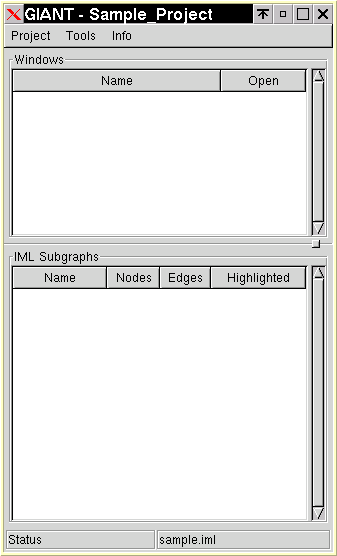
\includegraphics{gui/main_window}
   \caption{Main-Window}
   \label{Main-Window-Pic}
\end{figure}

%Erg�nzungen by Martin
Jede Instanz von GIANT hat genau ein Hauptfenster. \index{Hauptfenster}
Im Hauptfenster (siehe Abbildung \ref{Main-Window-Pic}) werden die
Anzeigefenster und
IML-Teilgraphen des aktuell ge�ffneten Projektes (siehe  
\ref{Project Persistenz der Projekte}) in Listen angezeigt. 
�ber Popup-Men�s k�nnen IML-Teilgraphen
und Anzeigefenster manipuliert werden.

Im Fenster befinden sich zwei Listen, Window List (2 Spalten), und
Subgraph List (4 Spalten).


  \subsection {Kopfzeile}
  In der Kopfzeile wird \gq{GIANT - <Projektname>} dargestellt.
 
  \subsection {Men�leiste (Main Window)}
  In der Men�leiste befinden sich folgende Eintr�ge:

    \subsubsection {Untermen� Project} \label{Main-Window-Project}
      \begin{enumerate}
         \item {New Project} % OK
         \item {Load Project}
         \item {Save Project}
         \item {Save Project As...}
         \item {Quit}
      \end{enumerate}    
      
     \subsubsection {Untermen� Tools}  \label{Main-Window-Tools}
       \begin{enumerate}
          \item {Delete Unreferenced Annotations}
          \item {Execute GSL Script}
        \end{enumerate}
        

    \subsubsection {Untermen� Info }  \label{Main-Window-Info}     
       \begin{enumerate}
          \item {About GIANT}
        \end{enumerate}
     

  \subsection {Statuszeile}
  \label{Statuszeile}
  \index{Statuszeile}
  Die Statuszeile befindet sich ganz unten im Hauptfenster. In der
  Statuszeile werden Informationen zum aktuellen Zustand von GIANT
  dargestellt.

   \subsection {Window List}
  
   Im Fenster befindet sich zuoberst eine Liste \gq{Window List}, welche
   alle Anzeigefenster des Projektes (offen und geschlossen anzeigt).
   
   \subsubsection {Inhalt Window List}
   \label{WINDOW-LIST}
   
   Window List hat die Spalten \gq{Name} und \gq{Open}. In
   \gq{Name} wird der Name aller Anzeigefenster dargestellt, in
   \gq{Open} befindet sich entweder ein Strich-Symbol (Fenster
   nicht ge�ffnet) oder ein H�kchensymbol (Fenster ge�ffnet).
    
    \subsubsection {Popup-Men� Window List}
    
    
        Beim Rechtsklick auf Window List �ffnet sich ein 
        Popup-Men� mit folgenden Men�punkten:
        \label{WINDOW-LIST-POPUP}

        \begin{enumerate}
          \item New Window % OK
          \item Open Window % OK
          \item Close Window % OK
          \item Save Window
          \item Delete Window % OK
          \item Rename Window % OK
        \end{enumerate}
    
  \subsection {Subgraph List}
  \label{GUI Subgraph List}
    
    Unter der Window List befindet sich eine Liste \gq{Subgraph List} �ber
    alle IML-Teilgraphen des Projektes.
   
    \subsubsection {Inhalt Subgraph List} 
    
      Subgraph List hat die folgenden Spalten:
      \begin{enumerate}
        \item Name
        \item Nodes
        \item Edges
        \item Highlighted
      \end{enumerate}
    
      In der Spalte Name stehen die Namen der existierenden IML-Teilgraphen,
      in Nodes die Anzahl der Graph-Knoten des jeweiligen IML-Teilgraphen, 
      in Edges die Anzahl der Graph-Kanten und in Highlighted befindet sich
      ein K�stchen in der
      Farbe, die f�r die Hervorhebung des IML-Teilgraphen verwendet wird
      (siehe hierzu auch \ref{hervorheben von Knoten und Kanten}).
      Bei nicht hervorgehobenen IML-Teilgraphen wird dieses K�stchen
      nicht angezeigt.

    
    \subsubsection {Popup-Men� Subgraph List}
    \label {Popup-Men� Subgraph List}
      Bei einem Rechtsklick auf Subgraph List �ffnet 
      sich ein Popup-Men� mit folgenden Men�punkten:
        \label{SUBGRAPH-LIST-POPUP}
        \begin{enumerate}
          \item Highlight (Men�)
            \begin{enumerate}
              \item Color 1
              \item Color 2
              \item Color 3
            \end{enumerate}
          \item Unhighlight In All Windows
          \item Copy IML Subgraph
	  \item Insert IML Subgraph
          \item Delete IML Subgraph
	  \item Create Window Selection % OK
          \item IML Subgraph Set Operation 
        \end{enumerate}   
        

\clearpage
\section {Anzeigefenster} \label{GUI Anzeigefenster}
\index{Anzeigefenster}

  \begin{figure}[!htbp]
     \centering
     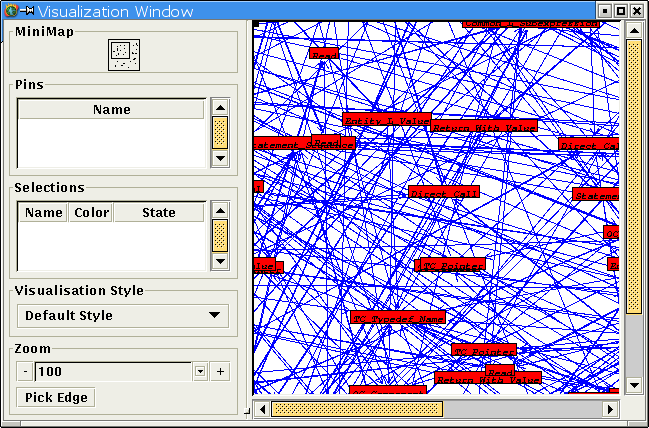
\includegraphics[width=16cm]{gui/visualization_window}
     \caption{Graph-Window}
     \label{Graph-Window-Pic}
  \end{figure}

  Im Programm kann es mehrere Anzeigefenster 
  (siehe Abbildung \ref{Graph-Window-Pic}) geben. 
  

  In Anzeigefenstern (Visualization Windows) werden Teile des IML-Graphen
  visualisiert.  Sie erscheinen im gro�en quadratischen rechten Teil
  (\gq{Vis Pane}) des Fensters. Die Vis Pane enth�lt den Anzeigeinhalt
  des Fensters.  Im linken Viertel des Fensters, der Toolbar
  (\gq{Vis Toolbar}) befinden sich untereinander die
  MiniMap, Pinliste, Selektionsliste, die Stilauswahl-Combobox und die
  Zoom-Kontrolle. 
  \index{Zoom-Kontrolle}
  \index{Visualisierungsstile!Stilauswahl-Combobox}

 \subsection {MiniMap} \label{GUI Minimap}
 \index{Minimap} 
 
 In der MiniMap wird der Anzeigeinhalt verkleinert dargestellt,
 der Graph wird jedoch nur durch einen grauen Kasten repr�sentiert,
 Knoten sind nicht sichtbar. Die MiniMap wird von einem Rahmen
 umschlossen. Der sichtbare Anzeigeinhalt wird durch einen kleineren
 Rahmen repr�sentiert, der innerhalb der MiniMap durch Mausklicks
 versetzt werden kann. Je nach Zoomstufe ist dieser Rahmen gr��er
 oder kleiner. Wird der Rahmen versetzt, wird der sichtbare Anzeigeinhalt
 in der Vis Pane entsprechend angepasst (siehe auch UseCase 
 \ref{Verschieben des sichtbaren Anzeigeinhaltes �ber die Minimap}).

  \subsection{Visualisierung der Knoten}

    In der Vis Pane werden die Fenster-Knoten und Fenster-Kanten angezeigt.
    
    Wenn auf einem Fenster-Knoten mit der rechten Maustaste geklickt wird, 
    �ffnet sich folgendes Popup-Men�:
 
    \subsubsection{Node-Popup-Men�}\label{Node-Popup-Men�}
    \begin{enumerate}
      \item Show Node Info Window
      \item Show Corresponding Source Code
      \item Move Node
      \item Annotation (Men�)
        \begin{enumerate}
          \item Add
          \item Change 
          \item Delete
          \end{enumerate}
      \label{Change Node Annotation}
      \label{Delete Node Annotation}
    \end{enumerate}
    
    Wenn in der Vis Pane mit der rechten Maustaste auf eine Stelle
    geklickt wird, an der kein Fenster-Knoten liegt, �ffnet sich das folgende
    Popup-Men�. Die Eintr�ge dieses Men�s sind auch im Node-Popup-Men�
    (siehe \ref{Node-Popup-Men�}) sichtbar.

    \label{Empty Vis Pane Right click}
    \begin{enumerate}
      \item Make Room % OK
      \item New Pin % OK
    \end{enumerate}
    

  \subsection{Pins} \label{VIS-PANE-Pins}
  \index{Pins}

    In der Pinliste (\gq{Pin List}) k�nnen Pins festgelegt werden.

    Im Popup-Men� der Pinliste befinden sich folgende Men�punkte:
    
    \begin{enumerate}
      \item Focus Pin % OK
      \item Delete Pin % OK
    \end{enumerate}

  \subsection{Selektionsauswahlliste} \label{Selektionsauswahlliste}
    Die Selektionsauswahlliste hat die Spalten \gq{Name} mit dem Namen der
    Selektion, \gq{Color} mit der Farbe der Selektion und \gq{State}
    mit dem Status der Selektion (eingeblendet oder ausgeblendet).

    Im Popup-Men� der Selektionsauswahlliste (\gq{Selection List}) befinden
    sich folgende Eintr�ge:

    \begin{enumerate}
      \item New Selection

      \item Move Selection
     
      \item Show Selection % war: Fade In Selection      

      \item Show all % Neu gemaess Daniel Simon

      \item Hide Selection % war: Fade Out Selection

      \item Layout Selection

      \item Create New IML Subgraph From This Selection % 
      
      \item Highlight Selection (Men�)
        \begin{enumerate}
        \item Color 1
        \item Color 2
        \item Color 3
        \end{enumerate}
	
      \item Unhighlight Selection % OK
        
      \item Zoom To Make Selection Fill Window % OK
     
      \item Copy Selection
      
      \item Copy Selection Keeping Existing Layout % OK
      \item Copy Selection Changing Existing Layout % OK
      \item Delete Selection % OK
      \item Delete Nodes and Edges of Selection
      \item Selection Set Operation % Changed by Martin
      
    %  \item Set Layout Algorithm For Selection --- deleted by Philipp
      
    \end{enumerate}    


  \subsection{Stilauswahl-Combobox}
  \label{GUI Stilauswahl-Combobox}   

    In der Stilauswahl-Combobox (\gq{Style Chooser}) kann ein 
    Visualisierungsstil (siehe auch \ref{Config Visualisierungsstile})
    ausgew�hlt werden.

  \subsection{Zoom-Kontrolle} \label{GUI Zoom-Kontrolle}  

    Die Zoom-Kontrolle besteht aus folgenden Elementen:
    
  \begin{enumerate}
      \item Button \gq{-} % OK
      \item Combobox mit vorgefertigten Zoom-Werten und Eingabem�glichkeit % OK
      \item Button \gq{+} % OK
      \item Button \gq{Pick Edge} % OK
  \end{enumerate}    

  In der ComboBox zur Zoom-Kontrolle befindet sich
  neben den vorgegebenen Zoomstufen \index{Zoomstufe} noch der
  Eintrag \gq{Fit in Window}.

    \subsection{Scrollbars}
    \label{Scrolleisten}
    
    Mit den beiden Scrollbars am unteren und rechten Rand des Anzeigefensters
    kann der sichtbare Anzeigeinhalt gescrollt werden.

\clearpage
\section{Knoten-Informationsfenster} \label{Knoten-Informationsfenster}

    \begin{figure}[!htbp]
       \centering
       \includegraphics{gui/node_information_dialog}
       \caption{Node-Info-Window}
       \label{Node-Info-Window-Pic}
    \end{figure}

    In Knoten-Informationsfenstern (siehe Abbildung 
    \ref{Node-Info-Window-Pic}) 
    k�nnen n�here Informationen zu Fenster-Knoten angezeigt werden.
    
    Im Knoten-Informationsfenster wird die ID und die Knotenklasse des 
    vom Fenster-Knoten repr�sentierten IML-Knotens dargestellt,
    darunter befinden sich untereinander die drei scrollbaren 
    Listen \gq{Attributes}, \gq{Successor Nodes} und
    \gq{Predecessor Nodes}.
    
    Unter den drei Listen befinden sich nebeneinander zwei Buttons
    \gq{Pick} und \gq{Close}. 
    Pick dient zur Auswahl eines anderen Fenster-Knotens 
    mittels des Fadenkreuzcursors. Die Informationen zu dem ausgew�hlten
    Fenster-Knoten werden dann im Knoten-Informationsfenster dargestellt
    (siehe hierzu auch UseCase 
    \ref {Details zu Knoten in einem bestehenden Informationsfenster anzeigen}).
    
    \subsection{Liste Attributes}
    
    Die Liste Attributes enth�lt die Attribute des Knotens und hat
    zwei Spalten:
    
      \begin{enumerate}
        \item Name  (der Name des Attributes)
        \item Value (der Attributwert)
      \end{enumerate}
    
    \subsection{Liste Successor Nodes}
    
      Die Liste Successor Nodes hat eine Zeile f�r jede vom Knoten abgehende
      Kante mit zwei Spalten:
    
    \begin{enumerate}
      \item ID (die ID des Nachfolger-Knotens)  
      %Changed by Martin Class -> Type da sonst Inkonsistent zu Abbildung
      %Eigentlich h�tte die Grafik ge�ndert werden m�ssen
      \item Type (die Kantenklasse der abgehenden Kante)
    \end{enumerate}    

    \subsection{Liste Predecessor Nodes}
      
      Die Liste Predecessor Nodes hat eine Zeile f�r jede beim Knoten eingehende
      Kante mit zwei Spalten:

      \begin{enumerate}
        \item ID (die ID des Vorg�nger-Knotens)
        %Changed by Martin Class -> Type da sonst Inkonsistent zu Abbildung
        %Eigentlich h�tte die Grafik ge�ndert werden m�ssen
        \item Type (die Kantenklasse der eingehenden Kante)
      \end{enumerate}

\clearpage
\section{Skriptdialog} \label{GUI Anfragedialog}

    \begin{figure}[!htbp]
       \centering
       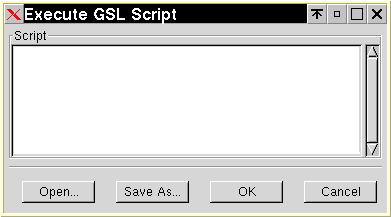
\includegraphics{gui/query_dialog}
       \caption{Skript-Dialog}
       \label{Skript-Dialog-Pic} 
    \end{figure}

Der Skriptdialog \gq{Query Dialog} (siehe Abbildung \ref{Skript-Dialog-Pic})
hat zuoberst ein Textfeld \gq{Query Text},
in das ein GSL Skript eingegeben werden kann.

Unter Query Text befinden sich folgende Buttons:

      \begin{enumerate}
        \item Open...
        \item Save As...
        \item OK
        \item Cancel
      \end{enumerate}
      
\clearpage
\section{Allgemeiner Texteingabedialog}
\label{DIALOG-WINDOW}

    \begin{figure}[!htbp]
       \centering
       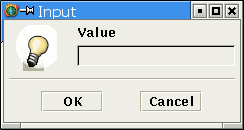
\includegraphics{gui/input_dialog}
       \caption{Dialog-Window}
       \label{Dialog-Window-Pic}
    \end{figure}

Ein allgemeiner Texteingabedialog ist ein Fenster Dialog Window 
(siehe Abbildung \ref{Dialog-Window-Pic}) mit dem
Titel \gq{Input}. Im Fenster ist ein einzeiliges Textfeld
mit einem Prompt-Text, zwei Buttons mit den Beschriftungen \gq{OK}
und \gq{Cancel}.

%\clearpage
\section{Set-Operation-Dialog}
\label{Common-Set-Operation-Dialog}

    \begin{figure}[!htbp]
       \centering
       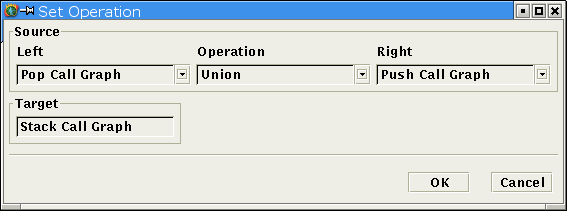
\includegraphics[width=16cm]{gui/set_operation_dialog}
       \caption{Set-Operation-Dialog}
       \label{Set-Operation-Dialog-Pic}
    \end{figure}


Der Set-Operation-Dialog (siehe Abbildung \ref{Set-Operation-Dialog-Pic}) 
dient dazu, Mengenoperationen �ber 
Selektionen und
IML-Teilgraphen durchzuf�hren.
Die Mengenoperation l�sst sich wie folgt beschreiben:\\
TARGET := LEFT\_SOURCE <op> RIGHT\_SOURCE \\


Bestandteile des Dialoges sind:
\begin {enumerate}

 \item LEFT\_SOURCE Combobox\\
 Soll eine Mengenoperation f�r Selektionen ausgef�hrt werden, so kann hier eine der
 Selektionen des entsprechenden Anzeigefensters ausgew�hlt werden.\\
 Bei einer Mengenoperation �ber IML-Teilgraphen, werden alle IML-Teilgraphen
 des Projektes angezeigt, von denen dann einer ausgew�hlt werden kann.
 
 \item <op> Combobox\\
 Mengenoperation, die ausgef�hrt werden soll; ausw�hlbar sind: Union, Difference oder Intersection.

 \item RIGHT\_SOURCE Combobox\\
 Soll eine Mengenoperation f�r Selektionen ausgef�hrt werden, so kann hier eine der
 Selektionen des entsprechenden Anzeigefensters ausgew�hlt werden.\\
 Bei einer Mengenoperation �ber IML-Teilgraphen, werden alle IML-Teilgraphen
 des Projektes angezeigt, von denen dann einer ausgew�hlt werden kann..
 
 \item TARGET Textfeld\\
 Name der neuen Selektion oder des neuen IML-Teilgraphen als Ergebnis
 der Mengenoperation.
 
 \item Buttons OK und Cancel\\
 Mit den beiden Buttons OK und Cancel l�sst sich die Operation starten bzw.
 der Dialog ohne Ausf�hren der Operation verlassen.
 
\end {enumerate}

 \clearpage
\section {Layoutalgorithmen Dialog}\label{Layoutalgorithmen-Dialog}

    \begin{figure}[!htbp]
       \centering
       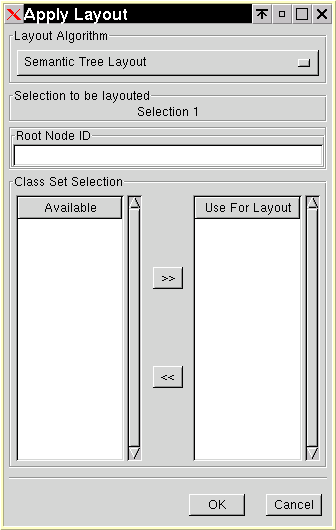
\includegraphics{gui/apply_layout_dialog}
       \caption{Layout-Algorithm-Dialog}
       \label{Layout-Algorithm-Dialog-Pic}
    \end{figure}

Der Layoutalgorithmen Dialog (siehe Abbildung \ref{Layout-Algorithm-Dialog-Pic}) 
bietet folgende M�glichkeiten:

\begin {enumerate}
 \item Auswahl des Layoutalgorithmus
 \item Ggf. Anzeige der zu layoutenden Selektion
 \item Ggf. Eingabefeld f�r die ID des Wurzelknotens bei Treelayouts
 \item {Eingabe der zu ber�cksichtigenden Klassenmengen bei semantischen Layouts,
 	Hierbei k�nnen mittels der Buttons \gq{>>} und \gq{<<} die 
        verf�gbaren
	definierten Klassenmengen zwischen den beiden
	Spalten \gq{Available} und \gq{Use For Layout} 
        hin und her geschoben werden.
	Nur Klassenmengen, die sich in der \gq{Use For Layout} Spalte befinden,
	werden f�r das Layout ber�cksichtigt.
        }
 \item OK Button
 \item Cancel Button
\end {enumerate}

\clearpage
\section{Dateneingabe}
Beschreibung von verschiedenen GUI Elementen zur Eingabe von Daten.

\subsection{Knoten-Annotations-Dialog}
\label{Knoten Annotations-Dialog}

    \begin{figure}[!htbp]
       \centering
       \includegraphics{gui/annotate_node}
       \caption{Node-Annotation-Dialog}
       \label{Node-Annotation-Dialog-Pic}
    \end{figure}
  
Der Knoten-Annotations-Dialog (siehe Abbildung 
\ref{Node-Annotation-Dialog-Pic}) besteht aus einem Fenster mit einem
Label, welches die ID des Knotens anzeigt, und einem Textfeld f�r den Annotationstext.
Mittels der beiden Buttons OK und Cancel k�nnen die �nderungen im
Textfeld �bernommen oder verworfen werden.  
\index{Knoten-Annotationen}


%  \clearpage
\subsection{Platz Schaffen-Dialog}
\label{Platz Schaffen-Dialog}

    \begin{figure}[!htbp]
       \centering
       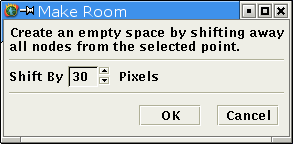
\includegraphics{gui/make_room}
       \caption{Make-Room-Dialog}
       \label{Make-Room-Dialog-Pic}
    \end{figure}

Im Dialogfenster Make Room (siehe Abbildung \ref{Make-Room-Dialog-Pic}) 
wird in einem Textfeld als Zahl 
eingegeben, um wie viel
Pixel die Fenster-Knoten an einer vorher markierten Stelle auseinandergeschoben 
werden sollen.
Mit dem Button OK kann best�tigt werden, mit dem Button Cancel abgebrochen werden.

\clearpage
\section{Ausgabe von Fehlermeldungen}
\label {GUI Ausgabe von Fehlermeldungen}

    \begin{figure}[!htbp]
       \centering
       \includegraphics{gui/error_dialog}
       \caption{Error-Window}
       \label{Error-Window-Pic}
    \end{figure}

Ein allgemeiner Fehlerdialog (siehe Abbildung \ref{Error-Window-Pic}) 
ist ein Fenster \gq{Error Window}
mit dem Titel \gq{Error}. Im Fenster befindet sich ein Label zur
Ausgabe der Fehlermeldung und ein Button mit der standardm��igen 
Beschriftung \gq{OK}. 
F�r weitere Informationen zum allgemeinen Fehlerverhalten von GIANT siehe auch
Abschnitt \ref{afa Fehlerverhalten}.

\section{Sicherheitsabfrage}\label{Sicherheitsabfrage}
\index{Sicherheitsabfrage}

    \begin{figure}[!htbp]
       \centering
       \includegraphics{gui/confirmation_dialog}
       \caption{Confirmation-Window}
       \label{Confirmation-Window-Pic}
    \end{figure}
    
Eine allgemeine Sicherheitsabfrage (siehe Abbildung \ref{Confirmation-Window-Pic}) 
ist ein Fenster (\gq{Confirmation Window}) mit dem
Titel \gq{Confirmation}. Im Fenster ist
ein Fragetext und ein Button mit der standardm��igen Beschriftung
Beschriftung \gq{Yes}, sowie ein Button mit der standardm��igen Beschriftung
\gq{No}. In dem Fragetext steht jeweils kontextabh�ngig 
die Information, die der  Benutzer zur Beantwortung der Sicherheitsabfrage
ben�tigt.

\clearpage

\section{Auswahl von Dateien}

  \subsection {Der \gq{Standard-Filechooser-Dialog}}
  \label {Standard-Filechooser-Dialog}

    \begin{figure}[!htbp]
       \centering
       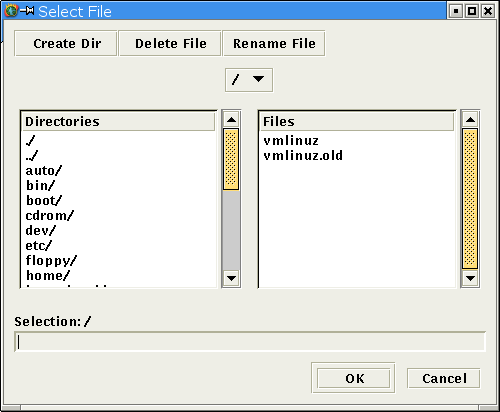
\includegraphics{gui/filechooser_dialog}
       \caption{Filechooser-Window}
       \label{Filechooser-Window-Pic}
    \end{figure}

Die Auswahl von Dateien (Laden/Speichern) passiert bei GIANT mittels
des Standard-Filechooser-Dialogs (siehe Abbildung \ref{Filechooser-Window-Pic}). 
Dieser Dialog ist Bestandteil der Widget-Bibliothek von GTK.


\section{Fadenkreuz-Cursor}
\label{Fadenkreuzcursor}
        Der Cursor verwandelt sich nach Auswahl bestimmter
        Funktionen (siehe z.B. UseCase \ref{Platz schaffen}) in ein Fadenkreuz.
        Durch Linksklick auf einen Fenster-Knoten oder eine 
        Fenster-Kante in einem Anzeigefenster  
        wird diese(r) f�r die jeweilige Funktion ausgew�hlt. 
        Der Fadenkreuz-Cursor wird auch zur Vorgabe von Positionen,
        an denen dann z.B. neue Fenster-Knoten eingef�gt werden,
        verwendet.
        Nach dem Linksklick  verwandelt
        sich der Fadenkreuz-Cursor wieder in den Standard-Cursor.
        Durch einen Rechtsklick bei aktivem Fadenkreuz-Cursor l�sst sich 
        die aktuelle Funktion abbrechen.


\section{Fortschrittsanzeige}
\label{GUI-Fortschrittsanzeige}
\index{Progressbar}


\label{Progressbar}
Es gibt in GIANT zwei M�glichkeiten zur Fortschrittsanzeige w�hrend
laufender Berechnungen.  Jede Progressbar ist mit \gq{The system is
busy. Please be patient.} beschriftet.

%\clearpage
\subsection{Progressbar-Runs}
\label{Progressbar-Runs}

     \begin{figure}[!htbp]
      \centering
      \includegraphics{gui/progressbar_busy}
      \caption{Progressbar-Runs}
      \label{Progressbar-Runs-Pic}
     \end{figure}

     Hierbei handelt es sich um ein Fenster mit einem sich bewegenden bzw. sich st�ndig 
     �nderndem Inhalt (z.B. ein Progress-Balken), so dass f�r den Benutzer erkennbar ist, 
     dass das System noch arbeitet 
     (beispielhafte Grafik siehe Abbildung \ref{Progressbar-Runs-Pic}).
  
%\clearpage
\subsection{Progressbar-Modal}
\label{Progressbar-Modale}      
     \begin{figure}[!htbp]
      \centering
      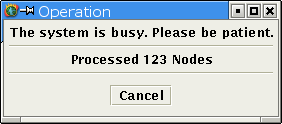
\includegraphics{gui/progressbar_cancel}
      \caption{Progressbar-Modal}
      \label{Progressbar-Modal-Pic}
     \end{figure}
     Der \gq{Progressbar-Modal}
     (siehe Abbildung \ref{Progressbar-Modal-Pic}) ist ein Fenster, 
     dass �ber den aktuellen Fortschritt
     einer Berechnung informiert, wobei der Gesamtaufwand unbekannt sein kann. 
     Hierzu wird kontinuierlich die Anzahl der schon bearbeiteten
     Datens�tze textuell ausgegeben, und, sofern bekannt, die Prozentzahl 
     der bereits
     bearbeiteten Datens�tze im Verh�ltnis zur gesamten Datenmenge.
     W�hrend dieser Dialog sichtbar ist, ist der Rest der GUI von GIANT
     gesperrt.
     Im Fenster existiert ein Button \gq{Cancel} \label{Progressbar-Modale-Cancel}, 
     mit dem eine laufende Berechnung abgebrochen werden kann.

%%% Local Variables: 
%%% TeX-master: "spec"
%%% End: 


%===============================================================================
% 
% Visualisierung des IML-Graphen
%
\chapter{Visualisierung des IML-Graphen}
\label{Visualisierung des IML-Graphen}

Dieses Kapitel beschreibt, wie IML-Knoten und IML-Kanten des
IML-Graphen innerhalb von Anzeigefenstern als Fenster-Knoten
und Fenster-Kanten dargestellt werden. Spezifiziert wird hier
das Ergebnis der Visualisierung, also das
Aussehen der Fenster-Knoten und Fenster-Kanten, nicht aber die Art und Weise,
wie GIANT diese Visualisierung erzeugt bzw.\ berechnet.

% ==============================================================================
%  $RCSfile: visulization.tex,v $, $Revision: 1.24 $
%  $Date: 2003-04-21 20:54:40 $
%  $Author: schwiemn $
%
%  Description:
%
%  Last-Ispelled-Revision: 1.17
%
% ==============================================================================


\section{Visualisierung von Knoten} 
\label{Visualization Visualisierung von Knoten} 

\index{Visualisierung!Knoten}
\index{Fenster-Knoten!Visualisierung}
Hier wird die Visualisierung eines Fenster-Knoten innerhalb eines 
Anzeigefensters beschrieben. Die tats�chliche Darstellung h�ngt
stark von der aktuellen Zoomstufe und dem gew�hlten Visualisierungsstil ab.

  \subsection {Knoten-Rechteck} \index{Visualisierung!Knoten-Rechteck}
  \label{Visualization-Knoten-Rechteck} 
  \begin {enumerate}
    \item
    Grundlage der Darstellung eines Fenster-Knotens ist immer ein Rechteck mit 
    fester, automatisch berechneter Breite. 
    
    \item
    Die H�he des Rechtecks h�ngt von der Anzahl der Attribute des 
    IML-Knotens, die direkt im Anzeigefenster dargestellt werden, ab. 

    \item
    Jedes Knoten-Rechteck hat eine konfigurierbare F�llfarbe und einen Rahmen, 
    dessen Farbe ebenfalls konfiguriert werden kann.
  \end{enumerate}

  \subsection {Knoten-Icon} \index{Visualisierung!Knoten-Icon}
  Jeder Fenster-Knoten kann �ber ein vordefiniertes Icon verf�gen, 
  welches im linken oberen Eck des Knoten-Rechtecks dargestellt wird. 
  Alle Fenster-Knoten f�r die kein Icon definiert wurde, 
  haben ein Standard-Icon.
  
  
  \subsection {Icon f�r Knoten-Annotationen} 
  \label{Visualsization Icon f�r Knoten-Annotationen} 
  \index{Knoten-Annotationen!Icon}
  Der Benutzer kann Fenster-Knoten annotieren. 
  Jeder Fenster-Knoten, f�r den so eine Annotation
  verfasst wurde, zeigt dies �ber ein entsprechendes Icon im
  Knoten-Rechteck an. \\
  F�r weitere Informationen zu Knoten-Annotationen siehe auch Abschnitt 
  \ref{Project Persistenz von Knoten-Annotationen}. 
  
  

  \subsection {Klassenname und ID} 
  \index{Visualisierung!Klassenamen}
  \index{Visualisierung!Konten ID's}
  Die ID eines IML-Knotens wird innerhalb des Knoten-Rechtecks rechts oben als
  Hexadezimalzahl angezeigt.\\  
  Der Name der Knotenklasse wird bei den Attributen angezeigt.

  \subsection {Attribute des Knoten} \index{Visualisierung!Attribute}
  Innerhalb des Knoten-Rechtecks k�nnen auch Attribute dargestellt werden 
  (Attributname und Wert), da das Knoten-Rechteck eine fixe Breite hat, 
  wird der zugeh�rige Text abgeschnitten,
  falls er zu lang ist. Dieses Abschneiden wird dem Benutzer durch das 
  Anf�gen von \gq{...} an das Ende des sichtbaren Teils des Textes 
  angezeigt.


\section{Visualisierung von Kanten}
\label{Visualization Visualisierung von Kanten} 

\index{Visualisierung!Kanten}
\index{Fenster-Kanten!Visualisierung}

\begin {enumerate}
  \item
  Fenster-Kanten sind immer 
  gerade Linien von einem Start- zu einem Zielknoten. 

  \item
  Fenster-Kanten k�nnen sich hinsichtlich ihrer 
  Linienfarbe und der Art der Linie 
  (z.B. gestrichelt oder durchgezogen) unterscheiden.

  \item \index{Schleifen} \index{Selbstkanten}
  Selbstkanten werden als kreisf�rmige Schleifen dargestellt.
\end {enumerate}

 
\section {Hervorheben von Fenster-Knoten und Fenster-Kanten}
\label{hervorheben von Knoten und Kanten}

\index{hervorheben von Knoten und Kanten}
\index{Fenster-Kanten!hervorheben}
\index{Fenster-Knoten!hervorheben}
Hier ist spezifiziert, wie Fenster-Knoten und Fenster-Kanten
hervorgehoben werden. Die genaue Art der Hervorhebung kann 
sich aber u.U.\ �ndern, wenn die Implementierung zeigen sollte,
dass ein anderes Vorgehen sinnvoller ist.


Innerhalb eines Anzeigefensters k�nnen
\begin {enumerate}
  \item die \gq{aktuelle Selektion},
  \item bis zu drei weitere Selektionen,
  \item und bis zu drei IML-Teilgraphen
\end {enumerate}
unterscheidbar hervorgehoben werden.


  \subsection {Hervorheben von Selektionen und der aktuellen Selektion}
  \label{Hervorheben von Selektionen und der aktuelle Selektion}
  \index{Selektionen!hervorheben}
  Beim Hervorheben der Fenster-Knoten und Fenster-Kanten 
  von Selektionen werden diese 
  mittels einer konfigurierbaren Farbe eingef�rbt.

    \begin {enumerate} 
      \item 
      Jeder Fenster-Knoten einer Selektion wird durch entsprechendes
      Einf�rben des Knoten-Rechtecks hervorgehoben.

      \item
      Geh�rt ein Fenster-Knoten zu mehreren Selektionen, 
      die hervorgehoben sind,
      so wird das Knoten-Rechteck entsprechend mehrfarbig eingef�rbt.


      \item 
      Jede Fenster-Kante wird dadurch hervorgehoben, 
      dass ihre Linie entsprechend
      dicker gezeichnet wird, wobei der Teil, um den die Fenster-Kante 
      verbreitert wird jeweils entsprechend eingef�rbt wird.

      \item
      Geh�rt eine Fenster-Kante zu mehreren Selektionen, 
      die hervorgehoben werden,
      so wird sie entsprechend weiter verbreitert und mehrfarbig eingef�rbt.

    \end {enumerate}


  \subsection {Hervorheben von IML-Teilgraphen}
  \label{vis Hervorheben von IML-Teilgraphen}
  \index{IML-Teilgraphen!hervorheben}

  \begin {enumerate} 
    \item 
    Jeder Fenster-Knoten eines IML-Teilgraphen wird dadurch hervorgehoben,
    dass er mit einem weiteren rechteckigen Rahmen versehen wird, 
    der entsprechend eingef�rbt ist.

    \item
    Geh�rt ein Fenster-Knoten zu mehreren hervorgehobenen IML-Teilgraphen 
    kommen entsprechend weitere Rahmen dazu.

    \item 
    Jede Fenster-Kante wird dadurch hervorgehoben, dass ihre Linie entsprechend
    dicker gezeichnet wird, wobei die der Teil, um den die Fenster-Kante 
    verbreitert wird, entsprechend eingef�rbt wird.

    \item
    Geh�rt eine Fenster-Kante zu mehreren IML-Teilgraphen, 
    die hervorgehoben werden, so wird sie entsprechend weiter verbreitert 
    und mehrfarbig eingef�rbt.

   \end {enumerate}  


\section {Detailstufen beim Zoomen} 
\label{Visualization Detailstufen}

\index{Zoomen!Detailstufen}
\index{Detailstufen}

\begin {enumerate}

  \item
  Beim Herauszoomen m�ssen Details abstrahiert werden. 
  Dies geschieht bei GIANT in mehreren Stufen.

  \item
  Eine exakte Spezifikation der Detailstufen, 
  insbesondere ab welcher Zoomstufe welche Detailstufe gew�hlt wird, 
  ist an dieser Stelle nicht sinnvoll. Optimale Parameter
  hierf�r werden im Laufe der Implementierung ermittelt.
  
  \item
  Beim Herauszoomen wird GIANT zuerst versuchen, die Gr��e der 
  Knoten-Rechtecke durch Verringerung der Schriftgr��e zu verringern. 
  Erst wenn die Schrift klein genug ist (aber noch gut lesbar) wird 
  GIANT Elemente der Darstellung der Fenster-Knoten entfernen.

\end {enumerate}

Es wird in etwa die folgenden Detailstufen geben.

  \subsection {Maximale Detailstufe}
  Bei maximaler bis hoher Zoomstufe (nahe ans Bild herangezoomt).\\
  Alle oben beschriebenen Bestandteile von Fenster-Knoten und Fenster-Kanten 
  werden angezeigt.\\
  Alle Beschriftungen in maximaler Schriftgr��e.

  \subsection {Sehr hohe Detailstufe}
  Nur die Schriftgr��e f�r Knoten- und Kantenbeschriftungen wird verringert. 

  \subsection {Hohe Detailstufe}
  Alle oben beschriebenen Bestandteile von Fenster-Kanten werden angezeigt.\\
  Bei Fenster-Knoten werden nur noch das Icon, der Klassenname und die ID im 
  Knoten-Rechteck angezeigt, die anderen Attribute aber nicht mehr.

  \subsection {Durchschnittliche Detailstufe}
  Die Beschriftungen von Fenster-Kanten werden nicht mehr angezeigt.\\
  Bei Fenster-Knoten enth�lt das Knoten-Rechteck nur noch das Icon.

  \subsection {Geringe Detailstufe}
  Bei sehr geringer Zoomstufe.\\
  Bei Fenster-Knoten wird nur noch das reine Knoten-Rechteck mit Rahmen und 
  F�llfarbe angezeigt (kein Icon mehr).

  \subsection {Minimale Detailstufe}
  Bei sehr geringer bis hin zur minimalen Zoomstufe.\\
  Die Knoten-Rechtecke werden immer kleiner gezeichnet, 
  bis sie ihre minimale Gr��e erreicht haben.
    
\section{Minimap} \index{Minimap}
Zu jedem Anzeigefenster gibt es genau eine Minimap, welche einen Bereich
des Anzeigeinhaltes als Rechteck abstrahiert darstellt. Dargestellt wird der 
Bereich des Anzeigeinhaltes, der einem alle Fenster-Knoten umspannendem
Rechteck entspricht.\\
Die Minimap bietet die folgende Funktionalit�t:
\begin {enumerate}

  \item 
   Der aktuell sichtbare Anzeigeinhalt wird auf der Minimap mit seiner 
   relativen Position und Gr��e im Verh�ltnis zum abstrahierten 
   Anzeigeinhalt dargestellt.

  \item \index{Scrollen!via MiniMap}
  �ber die Minimap kann auch gescrollt werden. Klickt der Benutzer
  auf einen Punkt innerhalb der Minimap, so wird der sichtbare
  Anzeigeinhalt automatisch auf den diesem Punkt entsprechenden
  Bereich des Anzeigeinhaltes gesetzt.  

\end {enumerate}

%%% Local Variables: 
%%% TeX-master: "spec"
%%% End: 


%===============================================================================
% 
% Nichtfunktionale Anforderungen
%
\chapter{Nichtfunktionale Anforderungen}

Hier werden die wesentlichen nichtfunktionalen Anforderungen an GIANT
spezifiziert. Insbesondere sind dies Anforderungen aus dem Bereich
des Software-Engineering, wie z.B. Wartbarkeit und Erweiterbarkeit.

% ==============================================================================
%  $RCSfile: nfa.tex,v $, $Revision: 1.12 $
%  $Date: 2003-04-18 00:50:12 $
%  $Author: keulsn $ 
%
%  Description: Nichtfunktionale Anforderungen
%
%  Last-Ispelled-Revision: 
%
% ==============================================================================

\section{Plattformunabh�ngigkeit}
\index{Plattformunabh�ngigkeit}
Das Produkt soll ein hohes Ma� an Plattformunabh�ngigkeit, wie sie sich aus der 
eingesetzten Entwicklungsumgebung ergibt, verf�gen 
(also alle Systeme auf denen GTK/ADA 1.2.12 lauff�hig ist). 
Explizit w�hrend der Entwicklung getestet und damit garantiert werden kann 
dies aber nur f�r Sun Solaris und Linux.

\section{Wartbarkeit}
\index{Wartbarkeit des Produktes}
Das System soll sich durch ein hohes Ma� an Wartbarkeit und Erweiterbarkeit 
auszeichnen. Erreicht werden soll dies durch die folgenden Grunds�tze.
\begin {enumerate}

  \item
  Wartbarkeit und Erweiterbarkeit gehen �ber Performanz.
  
  \item Strukturierung des Entwurfes nach Kriterien des
  Software-Engineerings.

  \item
  Strikte Trennung von GUI und Funktionalit�t.

  \item
  Einsatz von XML f�r alle editierbaren Konfigurationsdateien.

  \item
  Konfigurierbarkeit der Men�eintr�ge �ber eine XML Datei. Vorbehaltlich
  der Machbarkeit regelt der Entwurf hierzu n�heres.
 
\end {enumerate}


\section{Portabilit�t}
\index{Portabilit�t}

\begin {enumerate}

  \item
  Generell soll GIANT Betriebssystem unabh�ngig entworfen und Implementiert 
  werden.
  
  \item Weitere Ma�nahmen zur expliziten Unterst�tzung der Portabilit�t
  sind nicht vorgesehen.

\end {enumerate}

\section{Mengenger�st}
\index{Mengenger�st}
\index{Speicherverhalten}

\begin {enumerate}

  \item
  Ein explizites Mengenger�st, z.B. hinsichtlich der minimalen und 
  maximalen Anzahl von darstellbaren Fenster-Knoten, gibt es nicht. 

  \item
  Gr��enbeschr�nkungen (Gr��e der zu ladenden IML-Graph-Datei, 
  Anzahl Fenster-Knoten in einem Anzeigefenster ...) sollen sich alleine aus dem 
  verf�gbaren Arbeitsspeicher ergeben. 
   
  \item
  Falls der verf�gbare Arbeitsspeicher ersch�pft ist, soll das System nicht 
  abst�rzen, sondern vielmehr die entsprechende Aktion kontrolliert abbrechen 
  und dem Benutzer ein Weiterarbeiten erm�glichen.
\end {enumerate}

\section {Robustheit}
\index{Robustheit}
\begin {enumerate}

  \item
  GIANT soll m�glichst auf alle Fehler mit einer qualifizierenden Fehlermeldung
  reagieren und nicht unkontrolliert abst�rzen.

  \item
  Wo immer m�glich soll dem Benutzer nach Auftreten eines Fehlers ein sinnvolles
  Weiterarbeiten erm�glicht werden.

  \item
  Insbesondere bei Fehlern, die mit dem �berschreiten der verf�gbaren
  Hauptspeicherkapazit�t in Zusammenhang stehen, kann solch ein robustes 
  Verhalten nicht garantiert werden.
  
  \item 
  Speicherlecks k�nnen im Falle Abbruchs einer Aktion im
  Fehlerfalle nicht ausgeschlossen werden.

\end {enumerate}



\section{Robustheit gegen�ber �nderungen der IML-Graph-Spezifikation}
\index{IML-Graph-Bibliothek!robuste Anbindung}
Das System soll so an Bauhaus angebunden werden, dass �nderungen in der 
Spezifikation des IML-Graphen m�glichst keine Wartungsarbeiten erfordern. 
Besonders soll dies f�r die verschiedenen Attribute, 
Knoten- und Kantenklassen des Bauhaus-IML-Graphen gelten, 
da diese sich oft �ndern k�nnen.
Die Klassen und Attribute der Bauhaus-IML-Graph Bibliothek werden 
durch den IML-Browser nur so unterschieden, 
dass neu hinzukommende Attribute automatisch mit erfasst und damit 
angezeigt werden k�nnen.



\section{Leistungsanforderungen}
\index{Leistungsanforderungen}
\begin {enumerate}

  \item
  Bei GIANT handelt es sich um ein striktes Einbenutzersystem.
    
  \item
  Das Systemverhalten f�r den Fall, dass zwei Benutzer mittels verschiedener
  laufender Instanzen von GIANT (als Prozess im Betriebssystem) 
  gleichzeitig auf denselben Daten (Projekte und entsprechende 
  Verwaltungsdateien) arbeiten, ist undefiniert.

\end {enumerate}
  
  
   
\section{Antwortverhalten}
\index{Antwortverhalten}
\begin{enumerate}
 
  \item
  Bei Anfragen und Layoutalgorithmen kann keine maximale Rechenzeit garantiert
  werden. 
  
  \item
  Der Benutzer hat aber zu jeder Zeit die M�glichkeit, entsprechende
  Aktionen abzubrechen.
  

\end{enumerate}


\section{Sicherheit}
\index{Datensicherheit}

\begin{enumerate}

   \item
   Ein automatisches Schreiben von �nderungen etc. in die Projektdateien ist
   nicht vorgesehen, der Benutzer muss dies explizit veranlassen.\\
   Bevor Informationen verloren gehen (z.B. beim Beenden von GIANT) erscheint
   aber eine Sicherheitsabfrage.
   
   \item
   Muss GIANT auf Grund eines Fehlers beendet werden, so gehen alle bis dahin
   nicht persistent f�r das Projekt gespeicherten Informationen
   unwiederbringlich verloren.


\end{enumerate}


\section{Erweiterbarkeit}
\index{Erweiterbarkeit des Produktes}

Eine sp�tere Erweiterbarkeit von GIANT ist besonders hinsichtlich der im
Folgenden beschriebenen Funktionalit�t vorgesehen. Dies wird im Rahmen des
Entwurfes ber�cksichtigt.

\begin{enumerate}
  
\item Erweiterung um neue Layoutalgorithmen.
  
\item Erweiterung zur graphisch unterst�tzten Eingabe von
  GSL-Skripten.
  
\item \index{Kantenknickpunkte} Erweiterung um Kantenknickpunkte.

\end{enumerate}


%===============================================================================
% 
% Technische Produktumgebung
%
\chapter{Technische Produktumgebung}

Hier wird die zum Betrieb von GIANT n�tige Hardware 
und die n�tige Software spezifiziert.

% ==============================================================================
%  $RCSfile: technical.tex,v $, $Revision: 1.9 $
%  $Date: 2003-04-21 01:13:31 $
%  $Author: schwiemn $
%
%  Description: Hier sind die Anforderungen an die Programmumgebung 
%  spezifiziert. Dazu geh�ren die verwendete Hard- und Software, sowie
%  Schnittstellen zu anderen Produkten.
%
%  Last-Ispelled-Revision: 1.6
%
% ==============================================================================

\section{Software}
\index{Softwareanforderungen}
\index{Anforderungen!an die Software}
Das Programm stellt an die installierte Software folgende Anforderungen:
\begin{itemize}
  \item Sun Solaris oder Linux Betriebssystem
  \item Bauhaus Tools
  \item Emacs oder vi Texteditor
\end{itemize}


\section{Hardware}
\index{Hardwareanforderungen}
\index{Anforderungen!an die Hardware}
Das Programm l�uft auf SPARC Workstations und x86 kompatiblen PCs.
Im Folgenden sind die minimalen Hardwareanforderungen zur Arbeit mit kleinen 
und mittleren Projekten beschrieben. 
Bei gro�en Projekten ist ein Speicherausbau
von 2 GB und mehr empfehlenswert.

\subsection{Hardwareanforderungen SPARC}
\index{Sun SPARC}
\begin{itemize}
  \item UltraSPARC-II 300 MHz
  \item 512 MB Hauptspeicher
  \item 8 Bit Grafik mit einer min. Aufl�sung von 1024*786
  \item Maus mit mindestens zwei Tasten
\end{itemize}

\subsection{Hardwareanforderungen x86}
\begin{itemize}
  \item Pentium III 600 MHz
  \item 512 MB Hauptspeicher
  \item 8 Bit Grafik mit einer min. Aufl�sung von 1024*786
  \item Maus mit mindestens zwei Tasten
\end{itemize}

\section{Produkt-Schnittstellen}
\index{Schnittstellen}
\index{IML-Graph Bibliothek}
Das Programm soll in die Bauhaus Suite integriert werden k�nnen.
Als Schnittstelle dient dabei die Bauhaus IML Bibliothek. Weiterhin
kann die Verwendung von Kommandozeilenparametern und der GSL zur 
Integration in das vorhandene System genutzt werden.



%===============================================================================
% 
% Anforderungen an die Entwicklungsumgebung
%
\chapter{Anforderungen an die Umgebung}

Hier werden die wesentlichen Anforderungen an die Entwicklungsumgebung
von GIANT spezifiziert. Dies sind Werkzeuge, Programmiersprachen und
Bibliotheken, die bei der Entwicklung eingesetzt werden m�ssen, und
Standards, die beachtet werden sollen.
Spezifiziert wird hier auch die Sprache aller zum Lieferumfang von GIANT
geh�render Dokumente.

% ==============================================================================
%  $RCSfile: development.tex,v $, $Revision: 1.11 $
%  $Date: 2003-04-21 01:13:30 $
%  $Author: schwiemn $
%
%  Description:
%
%  Last-Ispelled-Revision: 1.5
%
% ==============================================================================

\section {Compiler und Bibliotheken} 
\index{Compiler}
\index{Bibliotheken}
\index{GTK/ADA}
\index{GNAT}
Das System soll in der Sprache Ada95 mit GNAT 3.14p entwickelt werden, 
wobei GTK/ADA 1.2.12 als graphische
GUI-Bibliothek eingesetzte werden soll. 
Das System baut auf der vom Kunden bereit gestellten IML-Graph-Bibliothek auf 
und soll des weiteren zur Unterst�tzung der Wartbarkeit m�glichst auch die 
vom Kunden zur Verf�gung gestellten 
Datenstrukturen (wie z.B. Hashtables aus Bauhaus/reuse/src) nutzen.

  
  \subsection {Lizenzrechtliches zu den Paketen des Kunden}
  \index{Pakete der Bauhaus-Reengineering GmbH}
  Folgendes gilt nicht f�r die IML-Graph-Bibliothek, sondern
  nur f�r die Datenstrukturen aus der \gq{Bauhaus Reuse Bibliothek}.\\
  Die vom Kunden zur Verf�gung gestellten Datenstrukturen 
  werden den Entwicklern von GIANT ohne lizenzrechtliche Bedingungen 
  �berlassen. Die Nutzungsrechte der Entwickler am Produkt GIANT werden 
  durch Einsatz dieser Datenstrukturen in keinster Weise ber�hrt.

 


\section {Einlesen und Schreiben von XML Dateien}
\index{XML Dateien}
Auf XML-Dateien soll mittels des DOM (Document Object Model) Parsers
aus XML/Ada 0.7.1 zugegriffen werden. XML/Ada 0.7.1 unterliegt lizenzrechtlich der \gq{GNAT Modified GNU Public
License} (GMGPL).\\
Als Alternative ist der XML-Parser aus GTK/Ada vorgesehen -- Paket Glib.XML.



\section {Sprache}
\index{Sprache der Dokumente}
Hier wird beschrieben, in welcher Sprache die einzelnen Dokumente
des Systems GIANT verfasst werden.

\subsection {Spezifikation}
Die Spezifikation -- dieses Dokument -- ist in deutscher Sprache verfasst.

\subsection {Benutzerhandbuch}
Das Benutzerhandbuch wird in deutscher Sprache verfasst.

\subsection {Entwurf}
Der Entwurf wird in Englisch verfasst.

\subsection {Interne Dokumentation}
Die interne Dokumentation von GIANT -- Kommentare im Quellcode --
erfolgt in englischer Sprache.

\subsection {Interaktion mit dem Benutzer}
\index{Interaktionssprache}
Die GUI von GIANT interagiert mit dem Benutzer ausschlie�lich in
englischer Sprache.

\subsection {Konfigurationsdateien}
Die Knoten und Attribute der XML-Konfigurationsdateien 
und der zugeh�rigen DTDs (Dokumenttyp-Definitionen)
werden mit englischen Bezeichnern benannt.





%===============================================================================
% 
% Begriffslexikon
%
\chapter{Begriffslexikon}

Das Begriffslexikon nennt Begriffe aus der \gq{realen Welt} und definiert
ihre besondere Bedeutung innerhalb dieser Spezifikation und darauf 
aufbauender Dokumente. Des weiteren wird hier die englische �bersetzung 
dieser Begriffe f�r alle englischsprachigen Dokumente von GIANT vorgegeben.

% ==============================================================================
%  $RCSfile: nomenclature.tex,v $, $Revision: 1.20 $
%  $Date: 2003-04-21 01:13:30 $
%  $Author: schwiemn $
%
%  Description: Begriffslexikon
%
%  Last-Ispelled-Revision: 1.14
%
% ==============================================================================

\begin{nomenclature}
  
  \term{Anfrage}{Query}{Eine Anfrage beschreibt einen Vorgang, bei dem
    �ber geeignete Kriterien IML-Konten und IML-Kanten aus dem IML-Graphen
    oder aus IML-Teilgraphen ausgew�hlt werden.}
  
  \term{Anzeigefenster}{Visualization Window}{Ein Fenster in dem ein
    Teilgraph des IML-Graphen nach bestimmten Kriterien visualisiert
    ist. Jedem Anzeigefenster ist ein Anzeigeinhalt zugeordnet.}
  
  \term{Anzeigeinhalt}{Window Content}{ Eine \gq{virtuelle} Oberfl�che
    auf der die Objekte des visualisierten Teilgraphen (also
    Fenster-Knoten und Fenster-Kanten) angeordnet sind, d.h. r�umliche
    Layoutinformation zu allen Objekten des entsprechenden
    Anzeigefensters. Abh�ngig von der Zoomstufe ist jeweils nur ein
    bestimmter Teil des Anzeigeinhaltes sichtbar - der sichtbare
    Anzeigeinhalt.  Die Gr��e des Anzeigeinhaltes ist theoretisch
    unbegrenzt.}
  
  \term{Fenster-Kante}{Window Edge}{Die graphische Repr�sentation einer
    IML-Kante innerhalb eines Anzeigefensters.}
  
  \term{Fenster-Knoten}{Window Node}{Die graphische Repr�sentation
    eines IML-Knoten innerhalb eines Anzeigefensters.}
  
  \term{Graph-Kante}{Graph Edge}{Eine Kante des IML-Graphen welche
    Bestandteil eines IML-Teilgraphen ist.}
  
  \term{Graph-Knoten}{Graph Node}{Ein Knoten des IML-Graphen welcher
    Bestandteil eines IML-Teilgraphen ist.}
  
  \term{IML-Graph}{IML Graph}{Der IML-Graph, wie er von der Bauhaus
    Reengineering GmbH gestellt wird.  Auf diesen Graphen wird �ber
    das sogenannte Reflection Model zugegriffen.}
  
  \term{IML-Kante}{IML Edge}{Eine Kante des IML-Graphen.}
  
  \term{IML-Knoten}{IML Node}{Ein Knoten des IML-Graphen.}
  
  \term{IML-Teilgraph}{IML Subgraph}{Eine Menge �ber Knoten und Kanten
    des IML-Graphen, die so gestaltet ist, dass sie einen Teilgraphen
    des IML-Graphen darstellt.}
  
  \term{Kantenklasse}{Edge Class}{Die Einteilung der IML-Kanten des
    IML-Graphen in verschiedene Klassen, wie sie sich aus der
    IML-Graph-Bibliothek von Bauhaus ergibt.\\
    Innerhalb dieser Spezifikation ist der Begriff Kantenklasse so
    zu verstehen, dass jede IML-Kante eindeutig zu genau einer Kantenklasse
    geh�rt, eine Vererbungshierarchie existiert nicht. Die Zuordnung
    einer IML-Kante zu einer Kantenklasse wird durch die Knotenklasse
    des Start-Knotens und den Namen des Attributes
    (aus dem Bauhaus-IML-Graphen), welches die IML-Kante
    beschreibt, festgelegt. Jede vorkommende Kombination aus der
    Knoten-Klasse eines Start-Knotens und dem Namen eines Attributes,
    welches eine Kante beschreibt, ist somit eine eigene Kantenklasse}

  \term{Klassenmenge}{Class Set}{Eine durch die IML-Graph Bibliothek
    vorgegebene Zusammenfassung von Kantenklassen und Knotenklassen.
    Es kann mehrere Klassenmengen geben. Die selben Knotenklassen und 
    Kantenklassen k�nnen gleichzeitig zu mehreren Klassenmengen geh�ren.}

  \term{Knoten-Annotationen}{Node Annotation}{Eine textuelle
    Beschreibung zu einem bestimmten Knoten des IML-Graphen.}
  
  \term{Knotenklasse}{Node Class}{Die Einteilung der IML-Knoten des
    IML-Graphen in verschiedene Klassen, wie sie sich aus der
    IML-Graph-Bibliothek von Bauhaus ergibt.\\
    Im Sinne der Verwendung dieses Begriffes innerhalb dieser Spezifikation
    liegt den Knotenklassen keine Vererbungshierarchie zu Grunde, jeder
    IML-Knoten geh�rt also eindeutig zu genau einer Knotenklasse}
  
  \term{Layout}{Layout}{Die zweidimensionale r�umliche Anordnung von
    Fenster-Knoten und Fenster-Kanten innerhalb eines Anzeigefensters
    auf dem sogenannten Anzeigeinhalt.}
 
  \term{Reflektion}{Reflection Model}{Die Schnittstelle zum Zugriff
    auf den IML-Graphen.}
  
  \term{Schleife}{Loop}{Eine Kante mit identischem Start- und Zielknoten.
    Wird oft auch als Selbstkante bezeichnet.}
  
  \term{Selektion}{Selection}{Eine Auswahl von Fenster-Knoten und Fenster-Kanten 
    eines visualisierten Teilgraphen des IML-Graphen innerhalb eines
    Anzeigefensters.}
  
  \term{Sichtbarer Anzeigeinhalt}{Visible Window Content}{ Der Bereich
    des Anzeigeinhaltes eines Anzeigefensters, der zur Zeit sichtbar
    dargestellt wird.}
  
  \term{Zoomstufe}{Zoom Level}{ Dieser Faktor beschreibt die Gr��e des
    sichtbaren Anzeigeinhaltes.  Bei einer sehr niedrigen Zoomstufe
    (auch: weit weg gezoomt) ist ein gr��erer Teil des im
    Anzeigefenster visualisierten IML-Graphen sichtbar als bei einer
    hohen Zoomstufe (auch: sehr nach heran gezoomt).}
  
  \term{hervorheben}{to highlight}{Hervorheben bedeutet, dass in einem
    Anzeigefenster visualisierte Fenster-Knoten oder Fenster-Kanten
    z.B.\ durch eine farbige Umrahmung von anderen Fenster-Knoten oder
    Fenster-Kanten unterscheidbar gemacht werden.}
    
  \term{selektieren}{to select}{Selektieren beschreibt einen Vorgang
    �ber den der Benutzer, z.B.\ durch Anklicken von Fenster-Knoten
    oder Fenster-Kanten mit der Maus, eine Selektion aufbaut.}

\end{nomenclature}

%%% Local Variables: 
%%% TeX-master: "spec"
%%% End: 


%==============================================================================
%
%  Index
%
\printindex

%==============================================================================
% 
% Anhang
%
\newpage
\appendix

\end{document}
